\documentclass[twoside,a4,12p]{report} %,draft,openright]


\usepackage{epsf,graphicx}
\usepackage{latexsym,amssymb}
\usepackage{setspace,cite}
\usepackage{graphicx}

\usepackage{caption}
\usepackage{subcaption}
\usepackage{hyperref}
\usepackage[]{algorithm2e}
\usepackage{amsmath}
\usepackage{gensymb}
\usepackage[usenames,dvipsnames]{xcolor}
\usepackage{tikz}
\usepackage{listings}
\usepackage{adjustbox}

% for margins left, right top bottom
\usepackage{anysize}
\marginsize{4cm}{2.5cm}{4cm}{4cm}

%\usepackage{draft} %draft option - doesn't put full figures in -
            % useful when editing

%does the headers on the pages - keep in
\usepackage{fancyhdr}

%omitting any of these makes the thesis compile without the omitted
%chapter - good for editing single chapters.
\includeonly{header,intro,background,appendix}

\begin{document}
\newpage

%Puts page numbering of preamble in roman and of main body of thesis in
%arabic. Also defines how chapters and sections are made
\pagenumbering{arabic}
\setcounter{page}{1} \pagestyle{fancy}
\renewcommand{\chaptermark}[1]{\markboth{\chaptername%
\ \thechapter:\,\ #1}{}}
\renewcommand{\sectionmark}[1]{\markright{\thesection\,\ #1}}

%DEFINES TITLE PAGE, and contains abstract, acknowledgements, etc.

%%%%%%%%%%%%%%%%%%%%%%%%%%%%%%%%%%%%%%%%%%%%%%%%%%%%%%%%%%%%%%%%%%%%%%%%%%%
% This is a sample header for a sample dissertation. Fill in the name,
% and the other information. LaTeX will work out the table of
% content, the list of figures and of tables for you.
%%%%%%%%%%%%%%%%%%%%%%%%%%%%%%%%%%%%%%%%%%%%%%%%%%%%%%%%%%%%%%%%%%%%%%%%%%%

\newpage
\thispagestyle{empty}

% ******* Title page *******
% **************************

\vspace*{2cm}
\begin{center}
{\Large\bf Automatic behavioural adaptation\\
			based on engagement assessment in\\
			child-robot interaction\\} \vspace{2cm} {\large
Fernando Garcia\\
\vspace{2cm}
Computer Human Interaction Learning and Instruction \\
\'Ecole Polytechnique F\'ed\'erale de Lausanne}

\end{center}

\vspace{7cm}
\begin{center}
{\large A Thesis Submitted for the Degree of \\MSc Erasmus Mundus
in Vision and Robotics (VIBOT) \\\vspace{0.3cm} $\cdot$ 2015
$\cdot$}
\end{center}
\singlespacing


%ABSTRACT
\begin{abstract}
Sustaining long-term interventions in a human-robot interaction scenario with an engaged user requires a system able to provide a suitable response depending on the context of the specific situation. It becomes a must to capture the significant \textit{passive} information provided by the user during the interaction. This evaluation has to be reliable enough to provide a variety of behavioral responses.

This work takes place in the context of the CoWriter project, the first known robotic agent which can engage a user in the learning by teaching paradigm for handwriting. By leveraging simulated handwriting on a synchronized tablet display, a Nao humanoid robot has been configured as a suitably embodied handwriting partner.

Additionally, the particularities of the project allow further research in terms of artificial intelligence for decision making. For instance, the ability to provide behaviours based on the engagement level, or the generation of responses based on the quality assessment of the handwriting provided by the user.

Two in situ experiments were scheduled with a primary school classes to evaluate the human-robot interaction outcomes of the system and their improvements with respect to the original version. Finally, long term experiments are currently in progress with the collaboration of a professional centre and under supervision of an ergo-therapist. 

\vspace*{5cm}



\begin{center}
\begin{quote}
\it The more important reason is that the research itself provides an important long-run perspective on the issues that we face on a day-to-day basis.
\end{quote}
\end{center}
\hfill{\small Ben Bernanke}

\end{abstract}

\doublespacing

%\pagestyle{empty}
\pagenumbering{roman}
\setcounter{page}{1} \pagestyle{plain}


\tableofcontents

\listoffigures
\listoftables

\chapter*{Acknowledgments}
\addcontentsline{toc}{chapter}
         {\protect\numberline{Acknowledgments\hspace{-96pt}}}

I would like to express my gratitude to my supervisor S\'everin Lemaignan who gave me not only the opportunity to work on this project, but also his knowledge and valuable advice. I would also like to extend my appreciation to Alexis Jacq, our doctoral assistant, for his constant willingness to help in each single stage of this work. Special thanks also to Sharma Kshitij whose statistical knowledge helped me in the results analysis of this research and I came to know about so many new things I am really thankful to him. Finally, I would also like to thank Dina for her constant support, patience and courage.
\pagestyle{fancy}


\newpage

%sets up headers for lefthand and righthand pages. To alter, edit
%these lines and the chaptermark/sectionmark lines above
\addtolength{\headheight}{3pt} \fancyhead{}
\fancyhead[LE]{\sl\leftmark} \fancyhead[LO,RE]{\rm\thepage}
\fancyhead[RO]{\sl\rightmark} \fancyfoot[C,L,E]{}
\pagenumbering{arabic}

%\singlespacing
%\doublespacing
\onehalfspacing
\chapter{Introduction} \label{chap:intro}

\section{Context} \label{sect:thefirst}

The CoWriter project aims to explore how a robot can help with the acquisition of writing skills. This project especially targets children, as handwriting difficulties in children at an early age often negatively affects the academic performance of the students \cite{christensen2005role} in addition to their self-esteem being adversely affected \cite{malloy1995handwriting}, causing them to shy away from expressing what they know \cite{medwell2008handwriting}. The use of robots in the learning activity presents an opportunity for the children to interact with an embodied, physical agent as part of the learning experience.
Furthermore, the use of robots in handwriting education comes with the potential to engage the child in meta-cognition through the learning by teaching paradigm, wherein a student takes the role of a teacher and experiences stronger educational benefits as a result (such as in \cite{palinscar1984reciprocal}).

A first prototype implemented by D.Hood et al. \cite{hood2015children} has shown good results in terms of robustness and functionality, becoming an appropriately-unskilled peer for a child to tutor. In this context, the CoWriter project is a teachable robotic agent developed to enhance the motivation, self-esteem and educational future of children with writing difficulties. However, there is still some challenges to be overcome in order to sustain long-term interactions with children, at the same time the progression of the writing is assessed properly. This project wants to push forward in this direction.

\section{Problem statement}
Children's engagement sustainability over time is one of the most important variables to make the process of learning effective \cite{umbach2005faculty}. It is well known that the role of the teacher \cite{smith2005pedagogies}, as well as the way the activity is formulated do matters in the learning efficiency. For instance, a child with difficulties who is trying to teach a robot how to write is more effective than a robot teaching a child (see section \ref{learningby}). In this sense, it would be possible to provide tools for the facilitators to assess the direction of the activity, or an activity change.
One of the most important challenges in human-robot interaction, or recently coined children-robot interaction, is the adaptivity of the agent taking into account the context of the interaction, modifying its outputs according to the information perceived from the environment and the user and providing eventually an adaptive emotional expression. This ability to adapt has been proved to be beneficial in long-term interactions \cite{tielman2014adaptive} \cite{lim2014mei} with children, manifesting a more positive attitude over time.

\section{Research question}
The research question addressed in this work has two main parts: The first one relates to the idea of providing an automatic behavioural adaptation based on the engagement assessment, and the second one implicit, how the level of engagement can be measured on real time.

\section{Approach}
The approach presented has been broken down into a number of sub-tasks for the project,
which are presented in different chapters. It starts reviewing the relevant literature to identify the state of the art in chapter \ref{chap:litReview} and it continues with the description of the development tools used provided in chapter \ref{chap:tools}. 
The core of the work starts trying to find an appropriate quantitative metric to assess if a shape is correct or not in chapter \ref{chap:correctness} since the intuition tell us that this output can be extremely useful along iterative sessions in order to see the progression of the user. In chapter \ref{chap:engagementModel} this correctness measurement is used to propose a first statistical model based on time responses to model student engagement.
Then, a second model based on a computer vision feature acquisition solution is proposed in chapter \ref{chap:systemOverview}. Moreover, this features acquired become helpful to create an adapting behaviour model using user's information. Finally, the design of the experiments are presented in chapter \ref{chap:feasibility} and the results in chapter \ref{chap:results}.

\section{Main contributions}
The main contribution of this work will be a robust metric to assess the shape correctness of the samples provided by the children. In addition, this metric will be used to provide a first engagement model based on writing times. Additionally, a second model using face features will be presented and evaluated showing results based on proximity and quantity of movement. However, the main contribution of this work is the adaptive behaviour model presented.



\chapter{Literature Review} \label{chap:litReview}

\section{The benefits of an adaptive behaviour state}

Children like robots, are more forgiving when a mistake or incoherence takes place. Moreover, they are quicker to ascribe human characteristics and personalities to robots \cite{beran2011understanding}. This is the reason behind the fact that child-robot interaction has enough potential to take place for a longer period of time. However, \cite{kanda2007two} has shown that for persistent interaction between a robot and a child, it is positive that the child establishes a social bond with the robot. 

Forming a social bond is a complicated process, and this can only be done through the expression of feelings, emotions and adaptive gestures. These expressions are very important in interactions and the forming of social relationships \cite{butler2003social}\cite{mcneill1992hand}. Hopefully, several studies, among them \cite{leite2012modelling} show that empathy facilities interaction in robot-child interaction, showing that human-based expressions can be successfully implemented by robots. Section \ref{models} goes deep in the current models for this topic.

Based on the previous statements, \cite{beran2011understanding} established that we can influence the expressive behavior of children by adapting the emotion expression of their robotic interaction partner. And the results obtained were that, children show more positive expressions with an affective robot. We can also state that children enjoy themselves more with a robot which shows adaptive behaviour expressions and gestures rather than with a robot which does not.

However, there are some constraints in the interaction to be taken into account. For instance, \cite{beran2011understanding} also established that children particularly prefer a robot which shows emotion through movement, whereas showing emotion through voice has the negative effect of reducing intelligibility.

\section{Behaviour expression models} \label{models}
In emotion research field there are two main established approaches. The first of them is based on distinguish several basic universal emotions such as happiness and sadness that implicitly assumes a discretization of the emotion. The second one considers an emotion to be a combination of two concepts: valence and arousal.
Arousal could be define as how exiting the emotion is, having several degrees of intensity whereas valence, would be how positive or negative the emotion is perceived. This approach as difference of the previous one, assumes a continuous space allowing the design of complex emotional states and smoothed transitions.
In both cases the models have some biological evidences. If we consider for instance a prolonged relaxed and quite situation without the influence of any external factor, new emotions take over the previous one within a certain period of time. However, external factors can make human switch from happiness to sadness: a bad new or a defeat for instance, as the first model suggests.
Therefore, the most important design choice is to have either a functional or a biological inspired approach. If we consider that the robot reacts directly from the environment, then it is functional but if it reacts according to its internal state, which is influenced by the environment, becomes biological inspired. Studies like \cite{schulte1999spontaneous} employs a state-machine based solution, but the recent tendency is to go towards a long-term interaction driven by the existence of an internal state \cite{hirth2011towards} \cite{canamero2001show}.
Tielman et al. for instance, proposed a model \cite{tielman2014adaptive} based on both by separation between gestures and emotion externalization consisting in four phases: an input phase, adapting the internal parameters based on this input, reasoning about the correct behaviour and the output to the robot. Recent works \cite{lim2014mei} focus more on a the feature acquisition from the environment. Features often related with the voice such as pitch volume or intensity.
However, another more complex models have been formulated. An example is \cite{velasquez1998modeling} which divides the releasers of emotion into four different complex neural mechanisms simulations: neural, sensorimotor, motivational and cognitive. In \cite{breazeal2003emotion} external events such as visual and auditory stimuli are sensed by the robot and are filtered by a number of feature extractors (e.g., color, motion, pitch, etc.). Then, in a high-level perceptual system, these features are bound by releaser processes that encode the robot's current set of beliefs about the state of the robot and its relation to the world.
\\
\section{The behaviour expression in child-robot interaction}

The use of behaviour and emotion externalization is a common resource to enhance interaction in educational, recreative and sometimes both contexts combined. The importance of this human feature is that relevant that several European projects, among them EMOTE\footnote{http://www.emote-project.eu/}, aims to improve the use of artificial tutors as learning-facilitator tools. The reason is that current platforms fail to engage the students in the same way a teacher does, as they lack the personal and empathy elements. Their research "explores how the exchange of emotional cues with an artificial tutor can create a sense of connection and act as a facilitator of the learning experience".
A commercial example of an interactive emotive robot is the owl ixi-play from WittyWorX (figure \ref{fig:int1}). It is an engaging robot buddy offering a simply playful interaction in the form of tangible games for early stage children. It is based on a peer situation where they play different games with in an active and adaptive manner. 
Pereira et al. in 2008 \cite{pereira2008icat} through an experiment consisting in to two scenarios: The first one, the user played against a physically embodied robotic agent (figure \ref{fig:int2}) and the second one, against a virtually embodied agent displayed on a screen proving that embodiment and emotion expression has implications on user enjoyment. 
The almost standard scenario of peer-to-peer set-up child-robot interaction, has evolved towards the inclusion of tactile displays that allows the execution of a rich number of activities equalizing the level of participation. An example is shown in figure \ref{fig:int3} from \cite{belpaeme2012multimodal}, an study carry out in the context of the project ALIZ-E.


\begin{figure}[h!]
        \centering
        \begin{subfigure}[b]{0.4\textwidth}
                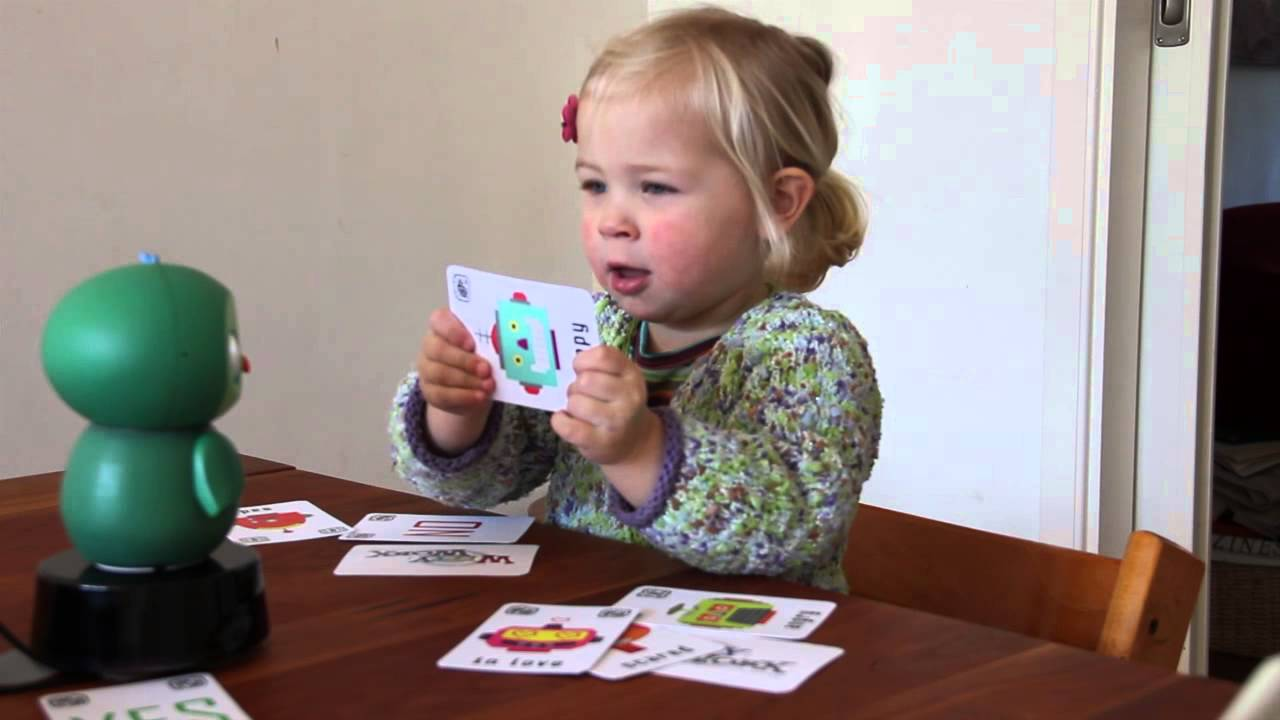
\includegraphics[width=\textwidth]{figures/int1.jpg}
                \caption{ixi-play}
                \label{fig:int1}
        \end{subfigure}%
        ~ %add desired spacing between images, e. g. ~, \quad, \qquad, \hfill etc.
          %(or a blank line to force the subfigure onto a new line)
        \begin{subfigure}[b]{0.475\textwidth}
                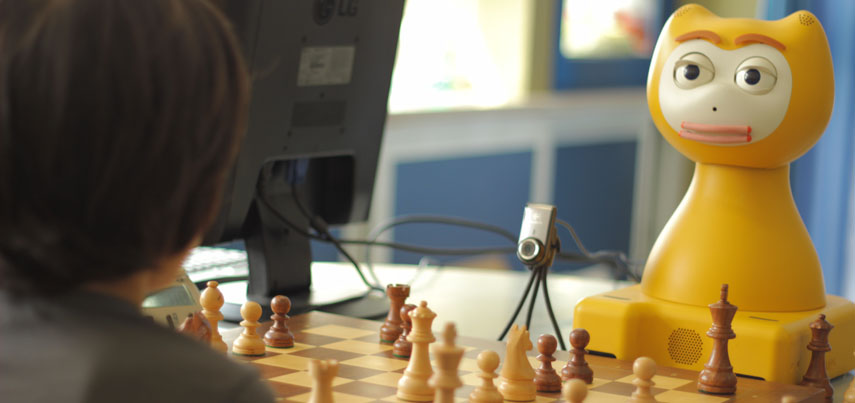
\includegraphics[width=\textwidth]{figures/int2.jpg}
                \caption{iCat}
                \label{fig:int2}
        \end{subfigure}
        ~ %add desired spacing between images, e. g. ~, \quad, \qquad, \hfill etc.
          %(or a blank line to force the subfigure onto a new line)
        \begin{subfigure}[b]{0.3\textwidth}
                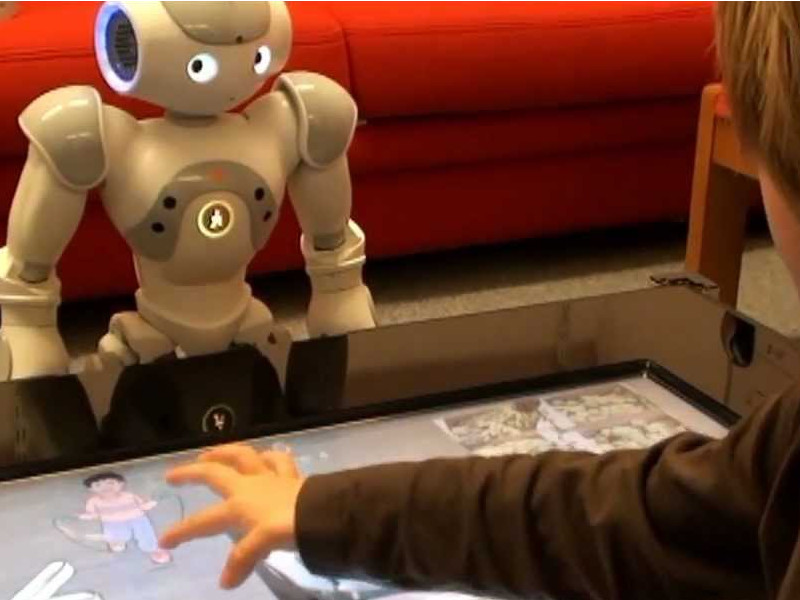
\includegraphics[width=\textwidth]{figures/int3.jpg}
                \caption{Nao}
                \label{fig:int3}
        \end{subfigure}
        \caption{Example results from emotion expression in child-robot interactions}\label{fig:animals}
\end{figure}

\section{The learning by teaching paradigm} \label{learningby}

In the learning by teaching paradigm, a student takes on the role of a teacher in order to teach
another student, and hopefully learns especially well as a result (such as in \cite{palinscar1984reciprocal}). Rohrbeck et al. \cite{rohrbeck2003peer} in their meta-analytic review of 81 peer tutoring programs in elementary schools, stated that peer-assisted learning interventions “effectively engage students in the learning process and produce academic gains across a variety of student populations, academic subjects, and classroom arrangements.”

Learning by teaching may be extended to involve a student teaching another who is not
a human, but rather a teachable agent which simulates a naive learner therefore motivating
students to teach it. Teachable agents have the benefits that they cause a student to reflect
on their knowledge and increase their ability of self-explanation; that they help the student to
structure/reorganize their knowledge; and that the student is promoted to take responsibility
of learning \cite{zhao2012learning}.

Okita and Schwartz \cite{okita2006observation} note that, given that a student has sufficient pre-understanding to interpret the actions of someone that they are observing, any discrepancies between what the student understands and what is seen in another’s actions may alert them to think more deeply about who is correct. It is reasonable to suspect that these discrepancies might not just be in the final result of the action observed: that is, when teaching another how to write, it may not just
be discrepancies in the final shape that act as a trigger for reflection in the teaching pupil, but
also the process of writing which was observed. This provides reasoning for having a teachable
agent which is sufficiently embodied so as to facilitate this.

While \cite{zhao2012learning} recommends the development of a teachable agent that is actively, rather than passively, engaged in the learning by teaching interaction, the increased learning gain results attained in \cite{okita2006observation} were done so even with the pupil being taught having been instructed to not contribute much information. This suggests that it may not be necessary, from a learning by teaching point of view, for the teachable agent to participate actively in the interaction to incite educational benefits. However, from an engagement point of view, this may not necessarily be true.

\section{The CoWriter project}
The CoWriter project\footnote{https://github.com/chili-epfl/cowriter\_letter\_learning/} involves the development of the first known robotic agent which can engage a user in the learning by teaching paradigm for handwriting. By leveraging simulated handwriting on
a synchronised tablet display, a Nao humanoid robot with limited fine motor capabilities is configured as a suitably embodied handwriting partner (see figure \ref{fig:cowriter}).

\begin{figure}[h!]
        \centering
        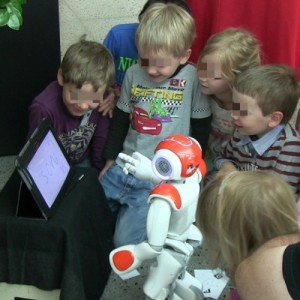
\includegraphics[width=0.4\textwidth]{figures/cowriter.jpg}
        \caption{CoWriter set-up.}
        \label{fig:cowriter}
\end{figure}

In order to achieve the simulated handwriting, shape models derived from principal component analysis of a dataset of letter trajectories are generated to parametrise written characters in a way that captures intuitively significant properties. Such a learning algorithm was developed, capable of incorporating feedback from users, both in terms of which generated letters are the best and from user demonstrations. Some of the most relevant tools used for the implementation of the system are reviewed in chapter \ref{chap:tools}.




\chapter{Review of Development Tools } \label{chap:tools}

\section{The Nao humanoid robot}

The robot available for the research is a Nao v5.0. The Nao is a humanoid robot, designed purposely to look approachable, which has been developed by Aldebaran-Robotics with the objectives of being affordable without sacrificing quality and performance \cite{gouaillier2008nao}. Indeed it brings access to an affordable (under 5K Euros) and performant biped robot to research laboratories and the mass market \cite{shamsuddin2011humanoid}, with 25 degrees of freedom, two cameras, speech capabilities and the ability to autonomously execute a range of tasks. Figure \ref{fig:nao_robot} illustrates the features of the Nao, including the 6 degrees of freedom in the arm: 2 at the shoulder, 2 at the elbow, 1 at the wrist and 1 for the hands grasping (open/closed) \cite{gouaillier2008nao}.

\begin{figure}[h!]
        \centering
        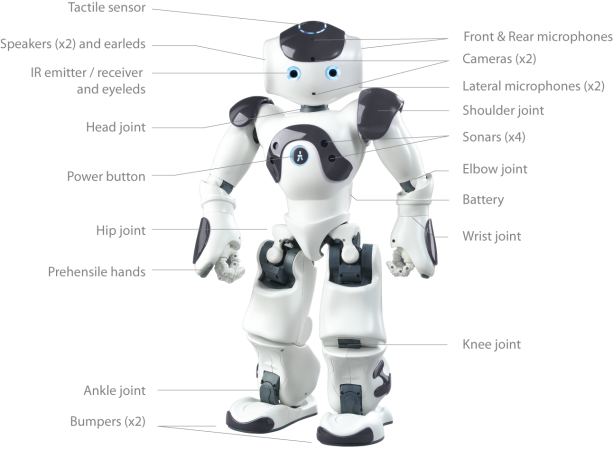
\includegraphics[width=0.5\textwidth]{figures/naoRobot.png}
        \caption{Nao features for v5.0 version \cite{aldebaran}.}
        \label{fig:nao_robot}
\end{figure}

\section{The NaoQI API}

NaoQi is the API provided by Aldebaran-Robotics to interface with the Nao. It is a modular
framework which can cope with a range of binaries developed in different languages, allowing
for a distributed environment which may be partly or wholly deployed on the robot \cite{gouaillier2008nao}. The level of abstraction available from the API includes execution of high-level autonomous behaviours such as causing the gaze of the robot to follow a ball, causing the robot to walk to a position, and causing the robot to stand after having fallen; and lower-level behaviours such as setting the joint values of the robot. A feature which is not present in the API, however, is an appropriate method for maintaining the robot’s relationship with other objects in the world, such as a tablet or a camera. For managing such information, the Robot Operating System has been employed.

\section{The Robot Operating System (ROS)}

Recognising that the required breadth of expertise for implementing software for a robotics
project is typically well beyond the capabilities of a single researcher, the Robot Operating
System (ROS) was developed to support large-scale software integration efforts \cite{quigley2009ros}. Its design criteria are listed as being peer-to-peer: allowing multiple hosts to be connected in a heterogeneous network rather than centralized to avoid unnecessary traffic flow; tools-based: where
small tools exist in different modules, arguably compensating for the loss in efficiency with the
gains in stability and complexity management; multilingual: where language-neutral messaging processing between modules allows mixing of different coding languages inside the modules and Free and Open-Source: with the full source code being made publicly available to facilitate the parallel design and debugging of different levels of the software \cite{quigley2009ros}.


\subsection{Framework}
In the ROS framework, nodes represent software modules, which communicate with each other
through messages over topics. Nodes should subscribe to relevant topics which they are interested in receiving messages over: a message can carry an arbitrary amount of data, structured into different fields (including, for example, arrays of other message types), and multiple nodes may be simultaneously publishing. Nodes can be connected to each other in a graph-like manner: the resulting graph may be arbitrarily complex, involving cycles, one-to-many or many-to-many connections. If a synchronous transaction is a more appropriate method of communication than the broadcasting exhibited by topics, a service may be used instead which has a defined request and response message format.

\subsection{Benefits}
In addition to those previously mentioned, the benefits of using ROS for robotics development
include that:
\begin{itemize}
\item Nodes may disconnect and reconnect to the network at run-time, allowing for ease in
debugging/prototyping of an experimental node amongst an existing framework of well-
debugged nodes by not requiring that they restart on changes to the node being developed.
\item Messages published can be logged for playback at a different time, without the need for
the nodes originally publishing the messages to be running. This is useful for software
development in research, where it is not desirable to connect all sensors to the system for
every test. In the case of interaction experiments, the messages may simulate the input
from a user interacting with the system which was captured in a once-off opportunity, for
offline analysis. ROS bags has been the perfect complement for the data recording.
\item Different frames of reference in a system, such as the position of grippers on a robot or an
object detected in space by a camera on the robot, can be related to each other through
a transformation tree which is generated dynamically by the tf transformation library. The ease of computing a transformation between two frames without needing to be concerned with the intermediate frames. Therefore, steps have been taken to continue using The ROS framework to interface with Nao 
\footnote{http://wiki.ros.org/nao\_robot} ). 
\end{itemize}

\section{The OpenCV library}
OpenCV\footnote{http://opencv.org} (open source computer vision) is the most popular open source library for Computer Vision related applications up to now, spanning from many very basic tasks like capture and pre-processing of image data, but also to high-level algorithms such as feature extraction, motion tracking or machine learning. It is released under a BSD license and hence it’s free for both academic and commercial use. It has C++, C, Python and Java interfaces and supports Ubuntu Linux. OpenCV was designed for computational efficiency and with a strong focus on real-time applications, fact that makes it perfect for the work presented in this document.

\section{The dlib library}
Dlib\footnote{http://dlib.net} is a general purpose cross-platform C++ library designed using contract programming and modern C++ techniques (including support for the most recent compilers). It is open source software and licensed under the BSD license. The most valuable asset that brings to the project is a robust real-time 2D face pose estimation, including features like; eyes, mouth, nose and eyebrows among others. The fact that it allow us to track precisely, even with occlusions or in poor light conditions, the face of the user in a range from $ -45\degree $  till $ 45\degree $ makes it suitable for this work. In addition, the library allows a flexible integration with OpenCV, through several methods for matrix and point conversions between both libraries. For these reasons, it has been used to track children's faces and features extraction.
\chapter{Assessing Shape Demonstration Correctness} \label{chap:correctness}
In a system whose main goal is to improve the handwriting of children with difficulties it is a must to be able to evaluate the progression over time for two main reasons: Providing a useful output of the child improvement to the activity supervisor and testing the efficiency of the system in the handwriting.  

\section{Motivation}
One of the main missing points in the current system is a proper metric to evaluate the demonstration provided by the user. Since people have the ability to assess intuitively when a letter is well written and when it is not, it becomes necessary to study a mathematical solution for a quantitative assessment when a child is performing an iterative task. Such outcome can be very useful for both the robot and the supervisor to adapt the behavior and to study the improvement of the children during the interaction or along several sessions, respectively. The goal of this stage of the project is to provide a suitable approach of inter-shape distance.
 
\section{Statistical shape modeling with PCA in the CoWriter}
The current system for the generation of the synthetic handwriting is based on a statistical shape modeling using Principal Component Analysis (PCA) \cite{stegmann2002brief} on the shape of the letters \cite{hood2015children}, whose basics will not be introduced in this work. 

By definition, the goal of PCA is to summarize the correlations among a set of observed variables with a smaller set of linear combinations. Because it is trying to capture the total variance in the set of variables, PCA requires that the input variables have similar scales of measurement, in our case being similar shapes. For instance, faces or samples of the same letter. But what is more important is that each component's eigenvalue represents how much variance it explains. 

In the case of the initial formulation of the CoWriter project several steps were accomplished in order to generate these shapes (the result is implemented in the \textit{shape learner\footnote{https://github.com/chili-epfl/shape\_learning}} python library). Firstly, the eigenspaces are generated over a set of letter paths captured from a digital pen and stored in a dataset (UJI Pen Characters 2) \cite{ujidataset}. Once a demonstration is provided by a child and projected to the correspondent letter eigenspace, it gets decomposed in their principal components. From this point new similar shapes can be generated by modifying the largest eigenvalues. Therefore, the robot response can be computed by modifying the eigenvalues towards midway between the child demonstration and a reference shape (a considerably good letter).

Based on the previous statements it is a must to capture as much variance as possible to properly provide similar shapes as the ones received from the user. However, this variance among same type of shapes can only be decoded if the eigenspace is able to capture it. In another words, the dataset used to build the eigenspace needs to be as rich as possible in terms of children mistakes variability. It was necessary then, to build a new dataset which includes that information, based on real children demonstrations.

Moreover, since the eigenspaces represent the main features of the letters, a good metric to compare two letters may be the Euclidean distance between their eigenvalues. For instance, in figure \ref{fig:datasets} can be observed the difference between the original dataset and the new one in terms of shape demonstration distances with respect to the reference shape. But also the difference when a new demonstration is included to the dataset for the generation of a new eigenspace (dynamic) or when it is not (static). In the case of the dynamic one, since after each demonstration shape the eigenspace is recomputed, we expect that the new eigenspace is able to capture more variance leading to greater distances between the demonstrations and the reference shape.

\begin{figure}[h!]
        \centering
        \begin{subfigure}{0.9\textwidth}
                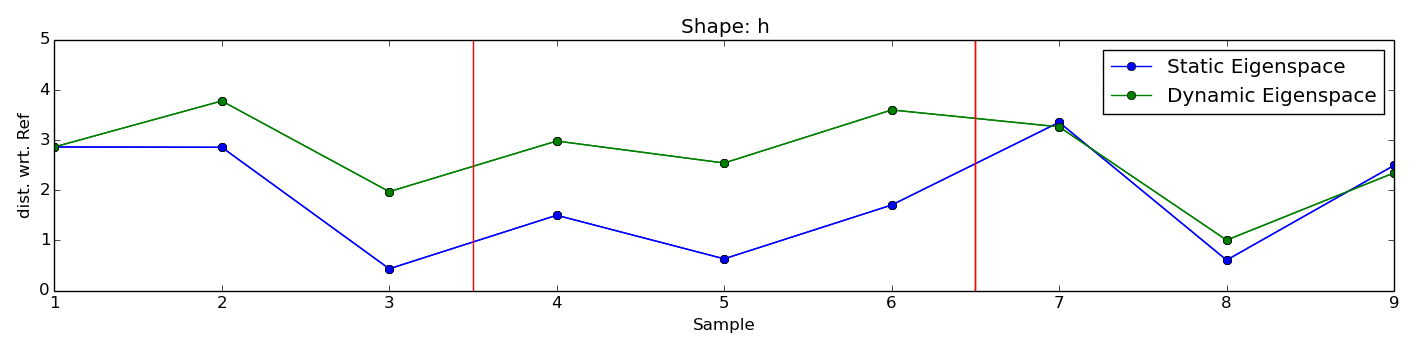
\includegraphics[width=1\textwidth]{figures/uji_pen.png}
                \caption{Uji pen dataset}
                \label{fig:ujipen}
        \end{subfigure}%

        \begin{subfigure}{0.9\textwidth}
                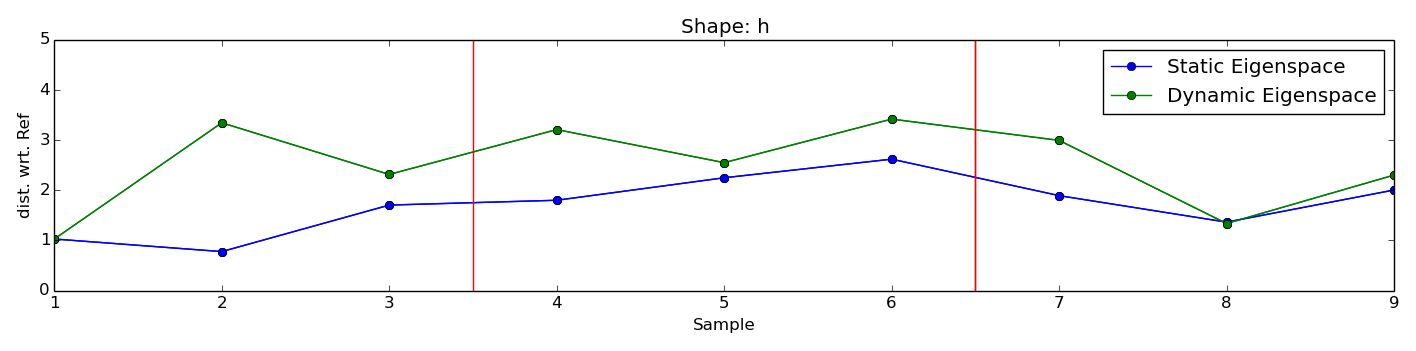
\includegraphics[width=1\textwidth]{figures/alexi.png}
                \caption{New dataset}
                \label{fig:alexi}
        \end{subfigure}
        \caption{Euclidean distance between the demonstration shapes and the reference shape in the eigenspace generated by the two datasets with (dynamic) and without (static) demonstration addition across different sessions (red lines)}
        \label{fig:datasets}
\end{figure}

In the case of \textit{uji pen} dataset (figure \ref{fig:ujipen}) we can see how in each iteration the distances of the demonstrations with respect to the reference shape has a higher variability in comparison with the \textit{new dataset} (figure \ref{fig:alexi}) which shows smoothed values (see blue lines). The reason is due to the greater variance captured by the second one. 
Furthermore, the distance between the demonstrations projected to a dynamic (green lines) and the ones projected to a static eigenspace (blue lines) remains smaller with the new dataset, getting reduced after certain amount of iterations. It suggests that the previous demonstrations did not induce a greater variance in the new eigenspace whereas in the old one did. Such results are provided using an Euclidean distance as metric. However, it is still remaining to be understood which metric can be more suitable to assess distances in the eigenspace in a reliable way. Examples would be City block distance or Mahalanobis distance among others.

\section{Uniform point distribution}  

From the acquisition of a user's demonstration till the generation of a shape response from the system, several steps were already implemented in the \textit{shape learner} library. Indeed, the shape generation pipeline has been improved in later revisions of the initial version. Currently, it includes several preprocessing steps before a shape is projected to the correspondent eigenspace and their values used for the shape generation. In figure \ref{fig:shapeProcess} the contribution of this section has been highlighted in the pipeline. 

\begin{figure}[h!]
        \centering
        
\includegraphics[width=1\textwidth]{figures/shapeProcess.png}
        \caption{Shape generation pipeline }
        \label{fig:shapeProcess}
\end{figure}

The current implementation of the system allows to capture the user input from the tablet in order to be processed and generate a similar shape in response. However, such points collected in the tablet need to be down-sampled to be independent from the time the tablet stylus remained on the screen surface. All shapes then, are reduced to 70 points using a cubic interpolation of a 1-D function.

In this way, it is necessary to normalize the shapes to become points located in between -1 and 1 to be processed (see equation \ref{eq:normalization}). Furthermore, in order to get the desired output, it is necessary to perform a point redistribution right after the correspondent normalization, due to the effect shown in figure \ref{fig:pointRedis}, otherwise the location of the shape in the eigenspace becomes distorted by the concentration of points in specific junctions or shape sides.

\begin{equation} \label{eq:normalization}
X' = X - (X_{max} - \frac{X_{max} - X_{min}}{2} )
\end{equation}

The uniformization is performed like in algorithm \ref{al:points} and its result it is shown in figure \ref{fig:pointRedis}.

\begin{figure}[h!]
        \centering
        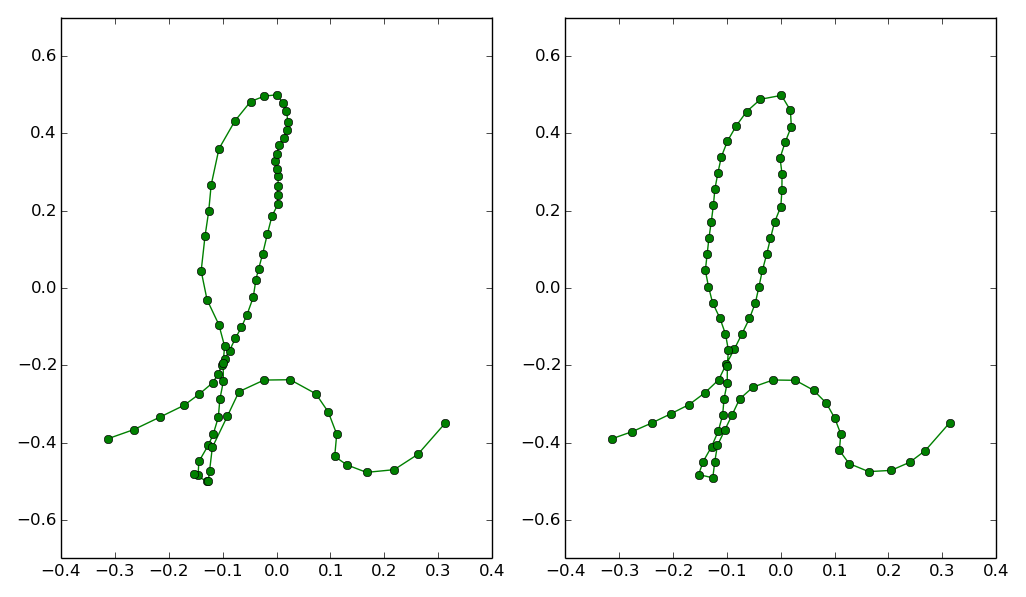
\includegraphics[width=0.9\textwidth]{figures/pointRedis.png}
        \caption{Before and after applying point redistribution}
        \label{fig:pointRedis}
\end{figure}
~
\begin{algorithm}[H]
 \scriptsize
 \While{$ i \leq numPointsShape $}{
   $ lengthShape = lengthShape + calcDist(points[i],points[i+1]) $\;
   $ scaleLength[i] = lengthShape $\;
   $ step = lengthShape / numPointsShape $\;
   $ j = 0 $\;
   \For{$ i= 0 \to numPointsShape-2 $}{
   		\While{$ i*step \geq scaleLength[j] $}{
   			$ j=j+1 $\;
   		}
   	$ j = j-1 $\;
    $ x0 = shape[j] $\;
    $ y0 = shape[j + numPointsShape] $\;
    $ x1 = shape[j + 1] $\;
    $ y1 = shape[j + 1 + numPointsShape] $\;
    $ diff = i*step - scaleLength[j] $\;
    $ dist = scaleLength[j + 1] - scaleLength[j] $\;
    $ newShapeX = x0 + diff*(x1-x0)/dist$\;
    $ newShapeY = y0 + diff*(y1-y0)/dist$\;
    }
  }
  \caption{Point uniformization algorithm}
  \label{al:points}
\end{algorithm}
\vspace{1cm}
By the use of this technique, we expect a better result in the decomposition of the shape in its eigenvectors and eigenvalues and thus, a more reliable correctness assessment using distance metrics in the eigenspace. Once the preprocessing is done, the demonstration shapes can be projected to the correspondent eigenspace obtaining a result similar to the one shown in figure \ref{fig:eigenspaces}. The shapes projected are shown in figure \ref{fig:shapeList}

\begin{figure}[h!]
        \centering
        \begin{subfigure}{0.4\textwidth}
                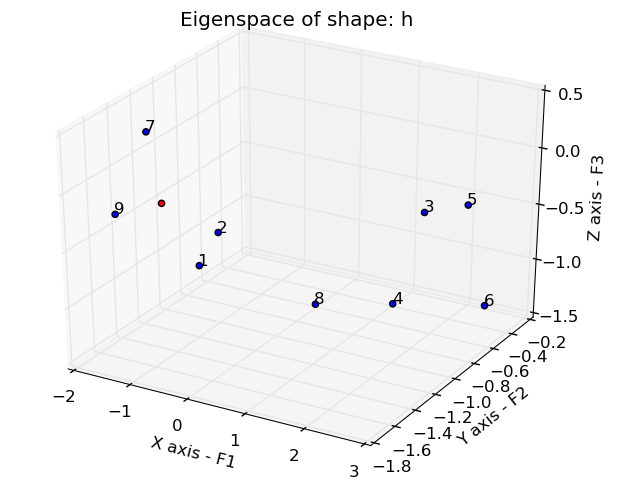
\includegraphics[width=1\textwidth]{figures/eigenBefore.png}
                \caption{Before}
                \label{fig:eigenBefore}
        \end{subfigure}
        \begin{subfigure}{0.4\textwidth}
                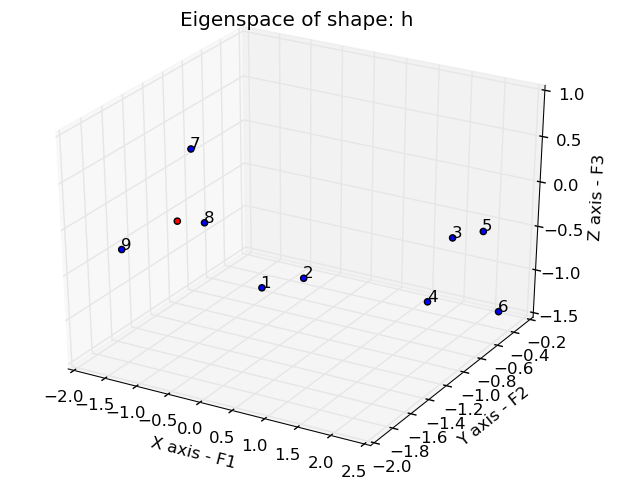
\includegraphics[width=1\textwidth]{figures/eigenAfter.png}
                \caption{After}
                \label{fig:eigenAfter}
        \end{subfigure}
        \caption{Demonstration shapes projected to the eigenspace with and without point uniformization (blue), and the reference shape (red).}
        \label{fig:eigenspaces}
\end{figure}


\begin{figure}[h!]
        \centering
        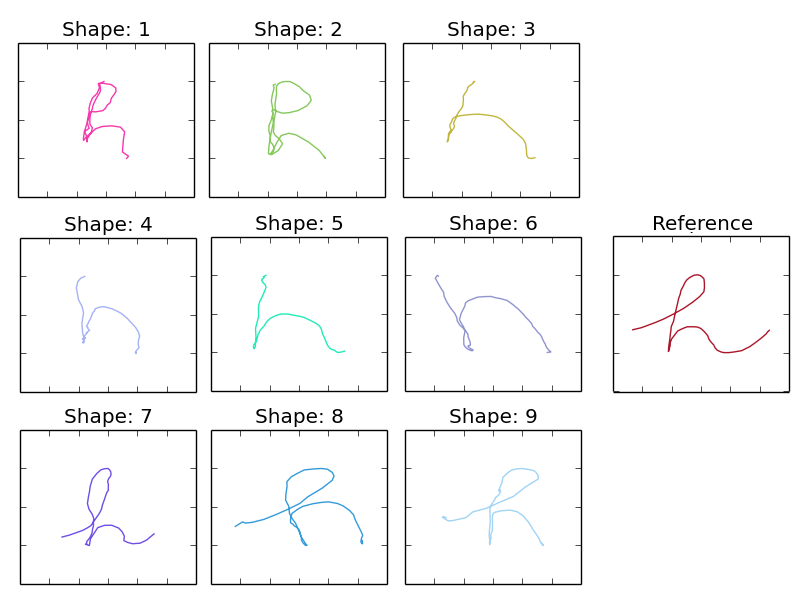
\includegraphics[width=0.7\textwidth]{figures/shapeList.png}
        \caption{List of shapes projected to the eigenspace}
        \label{fig:shapeList}
\end{figure}

We can observe how in figure \ref{fig:eigenAfter}, the preprocessing applied allows a correspondence between the qualitative and the quantitative assessment, locating shapes 7,8 and 9 together and closer to the reference one. Shapes 1 and 2 are located a bit farer since the samples show repeated strokes and finally, the different writing style shapes (3,4,5 and 6) are located far away from the reference.

However, choosing the appropriate metric and dataset to compose the eigenspace and project the shapes by itself does not assure a better distance assessment and thus a visual correctness correspondence shape-distance. At this point, it is necessary to know, first, if the types of shapes can be classified, and if it is possible, which clustering method would be more reliable for this task.


\section{Rating shapes using distance}
In order to rate the shapes provided by the user quantitatively and be consistent in the qualitative visual assessment, it has been necessary to test several methodologies; K-means using different distance metrics and SVM clustering method.
 
\subsection{Shape distance metrics in the eigenspace}  

In \cite{moon2001computational}, Moon and Phillips look at the effect of four traditional distance measures in the context of face recognition: City-block (L1 norm), squared Euclidean distance (L2 norm), angle, and Mahalanobis distance. 

\textbf{L1} City Block Distance
\begin{equation}
        d(x,y) = |x-y| = \sum_{i=1}^{k}|x_i - y_i|
\end{equation}

\textbf{L2} Euclidean Distance (Squared)
\begin{equation}
        d(x,y) = ||x-y||^2 = \sum_{i=1}^{k}(x_i - y_i)^2
\end{equation}

\textbf{Angle} Negative Angle Between Image Vectors
\begin{equation}
        d(x,y) = - \frac{x\cdot y}{\Arrowvert x\Arrowvert \Arrowvert y\Arrowvert} = -\frac{\sum_{i=1}^{k}(x_i - y_i)}{\sqrt{\sum_{i=1}^{k}(x_i)^2{\sum_{i=1}^{k}(y_i)^2}}}
\end{equation}	

\textbf{Mahalanobis} Mahalanobis distance
\begin{equation}
        d(x,y) = - \sum_{i=1}^{k} \frac{1}{\sqrt{\lambda_i}}x_iy_i
\end{equation}

Where $\lambda_i$ is the \textit{i}th Eigenvalue corresponding to the \textit{i}th Eigenvector. This is a simplification of Moon's definition:

\begin{equation}\label{eq:moore}
        d(x,y) = - \sum_{i=1}^{k} z_ix_iy_i \quad \textrm{where} \quad z_i = \sqrt{\frac{\lambda_i}{\lambda_i + \alpha^2}} \backsimeq \frac{1}{\sqrt{\lambda_i}} \quad \textrm{and} \quad \alpha=0.25
\end{equation}

Our experiments with the original formula showed poor results, hence our adoption of the definition in equation \ref{eq:moore}. Such experiments are summarized in table \ref{tab:distances} where K-means clustering method was used with different distance metrics.

\begin{table}[h!]
\centering
\begin{tabular}{l|l|l|l|l}
 		 		  & L1    & L2 & Angle & Mah \\ \hline	
Performance  	  & 77\% &  72\%  &	70\%   &  74\% 	    	

\end{tabular}
\caption{Distance metric performance for classification using K-means.}
\end{table}\label{tab:distances}

In this context K-means with L1 City block distance shown the best accuracy. Note that these results correspond to a test performed using 20 random samples of the same type of shape that were not previously used to compose the eigenspace. To conclude, we can consider the possibility, by performing K-means using City block distance, a simple metric for an automatized assessment of letter correctness if we assume there is only one cluster with reasonable good shapes.

\subsection{Shape classification}
In figure \ref{fig:shapeList}, three different types of shapes can be visualized with a certain correspondence in the eigenspace. In order to automatically classify the shapes, different clustering algorithms can be tested to check which one can provide better cluster segmentation based on the type of letter. For that, two common clustering algorithms were used: K-means using L1 distance since shows the best performance in table \ref{tab:distances} and Support Vector Machines (SVM).

The results summarized in table \ref{tab:clustering} were acquired using 34 shapes of 3 different letters from the same subject obtained along several experiments. There, we can see how SVM performs better in terms of classification.


\begin{table}[h!]
\centering
\begin{tabular}{l|l|l}
 		 		  & \textbf{K-means + L1}  & \textbf{SVM}	\\ \hline	
 \textit{h}-9 samples  	  &   100\% 	      &    100\% 	    \\ \hline
 \textit{a}-11 samples    &   81.8\%  	      &    90.9\%		\\ \hline
 \textit{g}-14 samples	  &   71.4\% 	      &    92.9\% 	     	

\end{tabular}
\caption{K-means - SVM classification performance comparison.}
\end{table}\label{tab:clustering}


\subsection{Additional outcomes}
As a secondary outcome of this chapter, a ROS Android app able to show the user shape progression across all repetitions was developed (see figure \ref{fig:plotApp}). It allows to provide a quantitative assessment of the user progression after each repetition in real time.

\begin{figure}[h!]
        \centering
        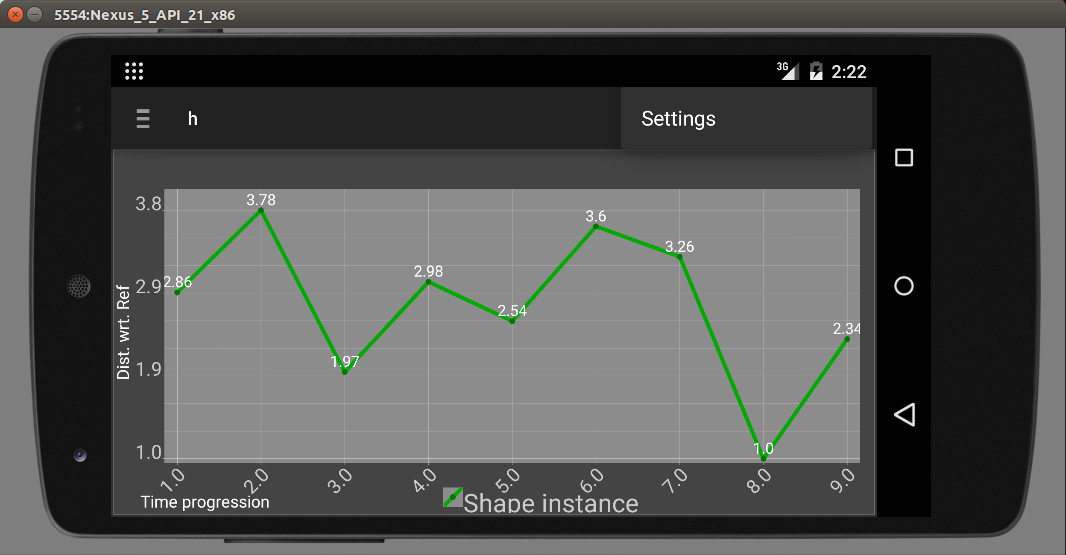
\includegraphics[width=0.8\textwidth]{figures/plotApp.png}
        \caption{ROS node App screenshot from Android Simulator that can be used to assess the user's  progression}
        \label{fig:plotApp}
\end{figure}


\chapter{Using Response and Writing Times to model Student Disengagement} \label{chap:engagementModel}

\section{Motivation}

In order to perform long term human-robot interactions in a educational context, it is important to know if the user is engaged on the task and if it is not, suggest an activity change. It is essential then, to have internal procedures that allow that. In \cite{joseph2005engagement} was established that time on task is an important predictor for how much students learn. Being also important that students are engaged during the learning process otherwise it will not be efficient. 

Therefore, we need to present a means for analyzing the response times and correctness of the student responses to model an overall level of engagement while using a computer tutor. This approach does not require humans to rate user interactions or measurements with biometric sensors since it can be measurable by statistical metrics. 

\section{Hypothesis}

Here, we hypothesize that a student who know how to write a shape would take less time to do it than someone who is not that skilled (who will take more to write the same shape). However, it is necessary to consider the children who wrote in a extremely short period of time. We can assume that students who spend less than a certain amount of time to write a shape are highly likely to be disengaged since they did not put time enough to write properly.

The fact that a user takes time to write a shape can not be taken as a sign of disengagement. So students who spent more time than a certain threshold are presumed to be just trying. Then, for purposes of building a model to predict a probability of disengagement, we consider only the regions R1, R2 and R3 present in figure \ref{fig:3pl}:

\vspace{5mm} %5mm vertical space

\begin{description}
  \item[Region 1] Performance at chance.
  \item[Region 2] Performance improve with time.
  \item[Region 3] Maximum of the performance
  \item[Region 4] Not considered
\end{description}

\begin{figure}[h!]
        \centering
        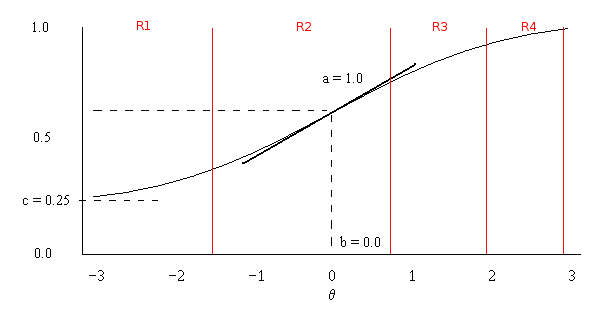
\includegraphics[width=0.6\textwidth]{figures/3PL.png}
        \caption{Three parameters logistic model from a item response function}
        \label{fig:3pl}
\end{figure}

The situation presented in figure \ref{fig:3pl} can be modeled by equation \ref{eq:itr}, the three parameter logistic (3PL) model which provides the probability of a correct response to a dichotomous item. In this equation the variable $\theta$ represents the student proficiency. The other three parameters control the shape of the logistic curve: \textit{a} is the discrimination which determines the steepness of the curve; and \textit{b} is the difficulty which controls the how much the curve is shifted from the axis center. Finally, \textit{c} is the guessing which sets the lower bound of the curve, in our case it is negligible since we assume the response can not be guessed blindly and still be correct.

\begin{equation}\label{eq:itr}
P(correct|\theta) = c + \frac{1-c}{1 + e^{-a(\theta-b)}}
\end{equation}

\section{Formal description time response-correctness }

Using Item Response Theory (IRT) \cite{embretson2013item} as starting point to model the relation between response time and engagement has used before in close questions assessment \cite{joseph2005engagement}. However, for shape writing follows a different procedure. In order to simplify the model we assume a dichotomy to assess if a shape is correct or not based on the distance to the reference shape introduced in chapter \ref{chap:correctness}.

However, the basic formula described in equation \ref{eq:itr} needs to evolve towards using a response time \textit{rt} as an input. In addition, discrimination and difficulty has to be calculated depending on the type of word used. For instance, to write a 3 characters word is not the same as writing a 5 characters one since takes a greater amount of time. It is also important to define an upper bound \textit{u} in the student's performance by a minimum distance to the reference shape that can be achieved. For instance, it is highly unlikely to obtain a correctness greater than 0.8.

The form of the new model is shown in equation \ref{eq:itr2}, where \textit{L} is the length of the word.

\begin{equation}\label{eq:itr2}
P(correct|rt,L) = \frac{u}{1 + e^{-a(-rt+b\cdot L)}}
\end{equation} 

In order to estimate \textit{a} and \textit{b} is necessary to do it separately for each length of word, since difficulty is highly accounted for that. Then, 3 character words are considered as \textit{easy}, 4 for \textit{moderate} and 5 for \textit{difficult}. For each model it is necessary to apply non-linear regression in order to obtain such unknowns. 

\section{Assessing correctness}
The model presented in figure \ref{fig:IRT} has been generated by collecting data from 10 adult people performing the writing of 5 different words with length $ L=3 $. Then, each of the letters of the same word was projected to the eigenspace and calculated its correctness (in terms of right or wrong setting a threshold) based on the distance to the reference letter. The mean of the three letters $ \bar{x} $ (see equation \ref{mean}) provides the result of a correct or incorrect word considering the condition shown in equation \ref{condition}.

\begin{equation}\label{mean}
 \bar{x}_{word} = \left ( \frac{1}{L}\cdot\sum_{i=1}^L{letter_i} \right )
\end{equation}

Then,

\begin{equation}\label{condition}
f(x)=\begin{cases}
 1, & \text{if $\bar{x}_{word} \geq 0.5$}.\\
 0, & \text{otherwise}.
\end{cases}
\end{equation}

where 1 and 0 are correct and incorrect word, respectively. As a final step, it is necessary to set the probability of a word to be correct given the response time. In order to do it, all samples have been grouped together by their writing response times in steps of 0.5 seconds, for instance two words written in 4.0 and 4.4 seconds would be grouped. Then, a mean criteria again was applied to decide the probability of being correct given a response time $P(correct|rt,L)$ comprise in the correspondent step (see green dots in figure \ref{fig:IRT}).

\begin{figure}[h!]
        \centering
        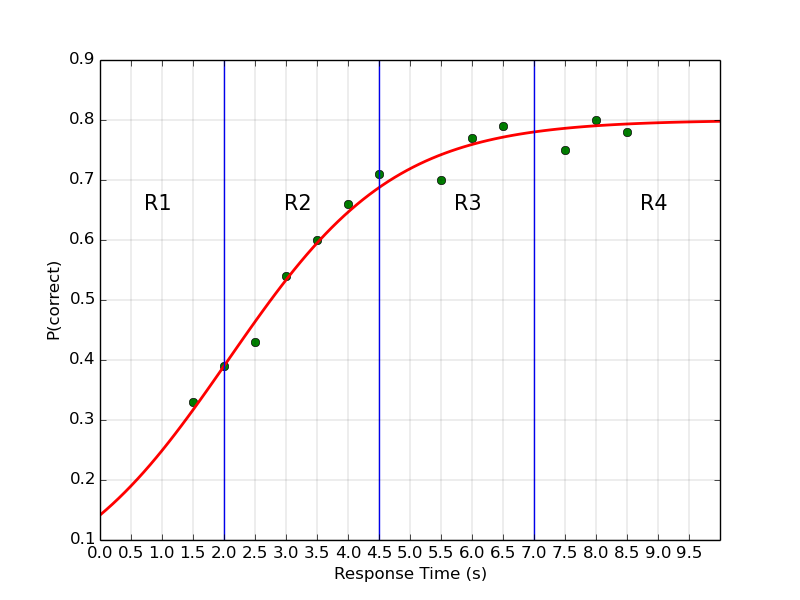
\includegraphics[width=0.6\textwidth]{figures/rt.png}
        \caption{Probability of being correct with respect to the response time}
        \label{fig:IRT}
\end{figure}

Finally, the results obtained for parameters \textit{a} and \textit{b} in a \textit{L=3} have been $ 0.7435 $ and $ 0.457 $ respectively.

\section{Disengagement estimation}
The current model can estimate the probability of a word to be correct given its writing time. However, to be able to calculate the engagement, it is necessary to assume that if a student is engaged, then he attempts to write the word with a maximum probability \textit{u} of being correct, which is the best performance in R3. This parameter is necessary since it is highly unlikely that the $ P(correct|rt,L) $ is higher than 0.8 and has been set based on a previous experiences. Therefore the model looks like in equation \ref{eq:irt3}

\begin{equation}\label{eq:irt3}
P_{disengaged} = \frac{u-P(correct|rt,L)}{u}
\end{equation}

For instance, someone who writes a word which has a length $ L=3 $ in a time $ rt=4 $ would obtain a $ P(correct|rt,L)= 0.67 $ so, $ P_{disengaged}=0.16 $ considering an upper bound $ u=0.8 $. And therefore, the probability of being engaged is $ P_{engaged}=1-0.16=0.84 $

\section{Limitations}
Despite generating a reasonable model, it presents some limitations. The main drawback of this method is the way to account for differences among students. But mainly, the model has not been tested so far, since the experiments carry out involved children around 5.5 years old and most of the time during the experiment they were trying to copy the shape models provided as helping material. Therefore, correctness and time responses were not obtained properly and were not suitable for the purpose of model training and testing.

In order to design a study were the present model can be tunned properly, it would be necessary to reproduce the experiments with 7 years old users with handwriting knowledge but with difficulties to perform it. In addition, it would be necessary to test the model to extract partial correlations between the disengagement measurements and learning gains after each iteration.  


\chapter{Adapting Behavior} \label{chap:systemOverview}

The implication of a physical agent, like Nao, in a human-child interaction context provide several benefits (see chapter \ref{chap:litReview}). It is important to be able to use all resources such as arms, head and other in an adaptive and flexible way without modifying the essence of the main activity, the writing. Therefore, the final goal of an adaptive behaviour is to smooth the interaction with the purpose to make children show more positive attitude towards the activity presented \cite{lim2014mei}\cite{tielman2014adaptive}. In this sense, an adaptive emotion expression system was developed based on internal valance and arousal values influenced by the current state of the interaction partner.

In addition, most of the visual information extracted from the user during the interaction will be recorded and used to assess the level of engagement. Therefore, we hypothesize that some of the features captured such as quantity of movement, proximity or gaze direction can be identifiers of the engagement level in this specific interaction context. The results related to this second part are shown in chapter \ref{chap:feasibility}.

\section{The valence and Arousal model}
	
The valence-arousal model has been widely spread as a simple standard for emotion detection and modelling in the literature \cite{russell1980circumplex}. Valence refers to how positive or negative an event is, and arousal reflects whether an event is exciting or calming, agitating or soothing. In this case, this technique is applied to enrich the variety of behaviours expressions based on online factors coming from the user interacting.

The main principle of the model is the need to be feed with external information which is encoded along two dimensions, \textit{valence} and \textit{arousal}. These dimensions are represented on a scale from -1 to 1 and are used to physically modify the current behaviour of the robot. For instance, when the child smiles to the robot, the current emotion indicator moves towards \textit{happiness} encoded in the map shown in figure \ref{fig:vaMap}.

\begin{figure}[h!]
        \centering
        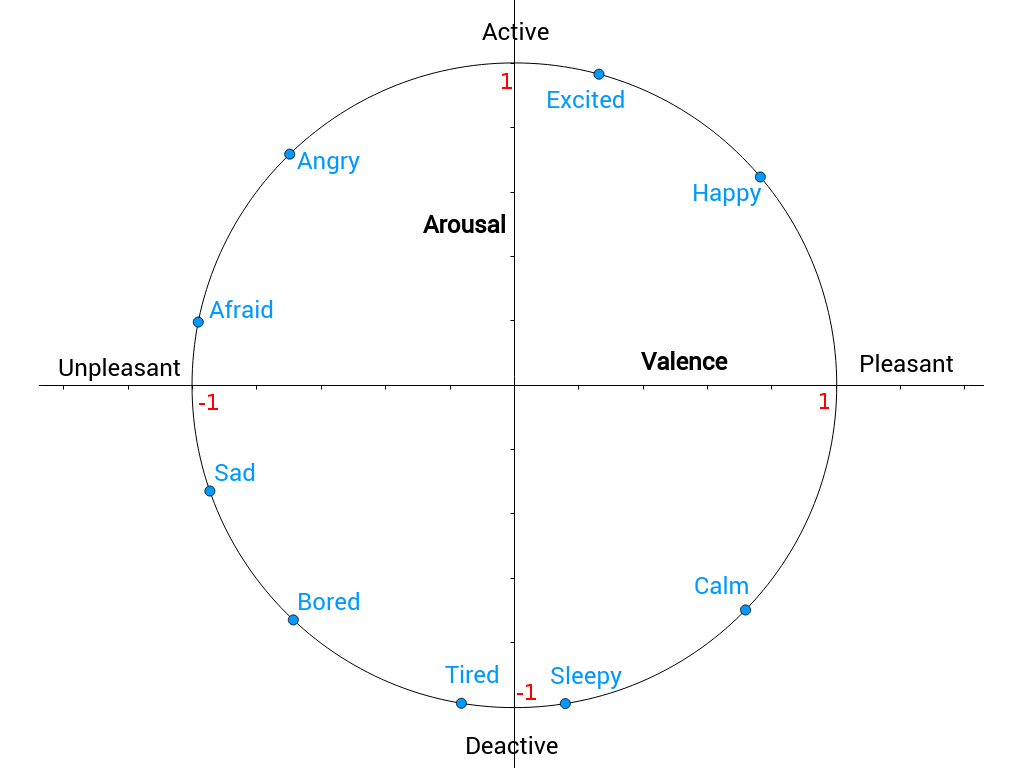
\includegraphics[width=0.6\textwidth]{figures/vaMap.png}
        \caption{Valence-Arousal map \cite{bradley1999affective}}
        \label{fig:vaMap}
\end{figure} 
  
\section{System Overview} \label{SystemOverview}

In order to capture the appropriate cues from the children with the purpose of generating an emotion content in a 2D map, we relied on \textit{dlib} library. This resource, in combination with the tools offered by OpenCV, provide the sufficient robustness to reliably acquire user faces. Once the acquisition tools and the behaviour model are established, it is necessary to define the possible visual relevant cues: 

\begin{itemize}
  \item Proximity to the scene.
  \item Quantity of movement (QoM).
  \item Gaze direction.
  \item Saliency.
  \item Beaming.
\end{itemize}

And the generation of a set of behaviours on the humanoid robot Nao based on the following actuators:

\begin{itemize} \label{listResources}
  \item Head pitch
  \item Left and right shoulder roll and pitch.
  \item Left and right elbow roll.
  \item LED eye color.
  \item Pitch and volume voice.
\end{itemize}

The main challenge is to combine the behaviour adaptation together with other independent activities since in both cases resources such as arms or head are shared between them. It is a must not to collide with the current activity but still adapt the behaviour of the robot on real time. At this point the implementation of the system plays an important role. It has been divided in three ROS nodes; the \textit{vision} manager, the \textit{emotion manager}, and the \textit{action} manager. The framework is designed in such a way that its execution is independent from the original CoWriter, acting as a modifier and activity independent (see figure \ref{fig:system}).

\bigskip

\begin{figure}[h!]
        \centering
        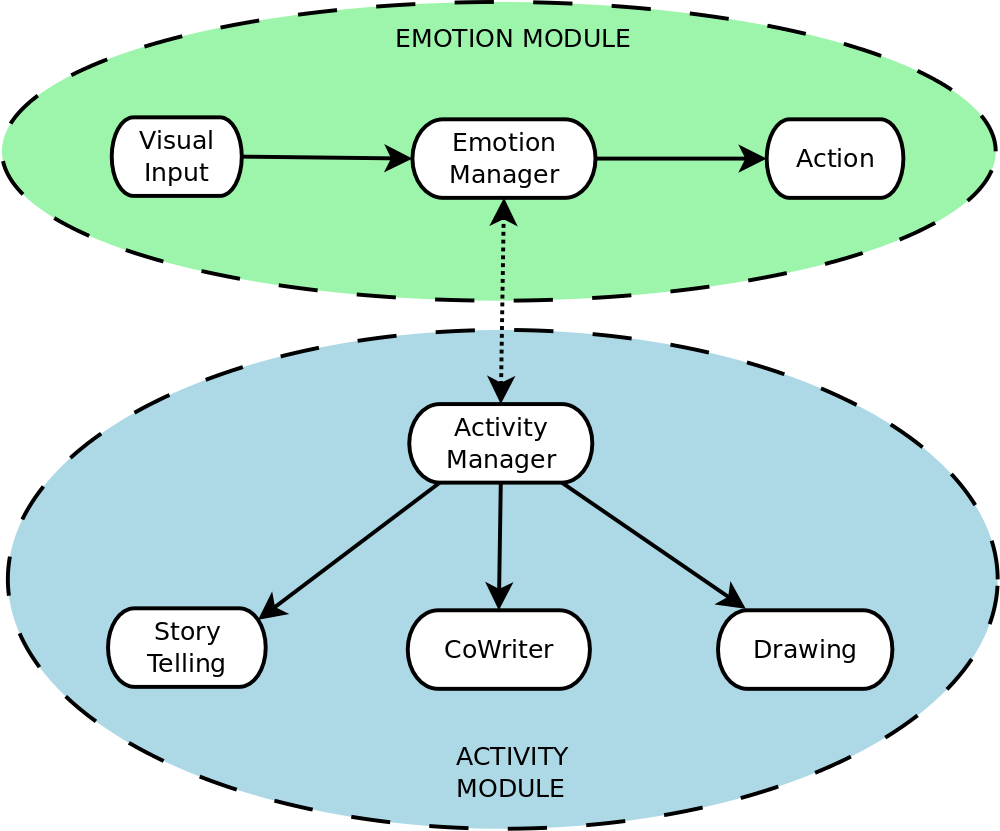
\includegraphics[width=0.5\textwidth]{figures/system.png}
        \caption{Independent emotion (green) and activity (blue) frameworks}
        \label{fig:system}
\end{figure}

\bigskip

The \textit{vision} node is written in C++ and contains all computation related with the image acquisition and processing using both OpenCV and \textit{dlib}. It publishes to the \textit{emotion manager} node which integrates all the information received and generates a resultant vector (valence-arousal) towards the correspondent emotion. Finally, the \textit{action} node performs the necessary movements to embody the emotion at the specific time. A deeper overview of the system is shown in figure below.

\begin{figure}[h!]
  \begin{adjustbox}{addcode={\begin{minipage}{\width}}{\caption{%
      Structure of the ROS nodes used to implement the system. Ovals represent nodes, arrows represent messages, and rectangles message topics.
      }\end{minipage}},rotate=90,center}
      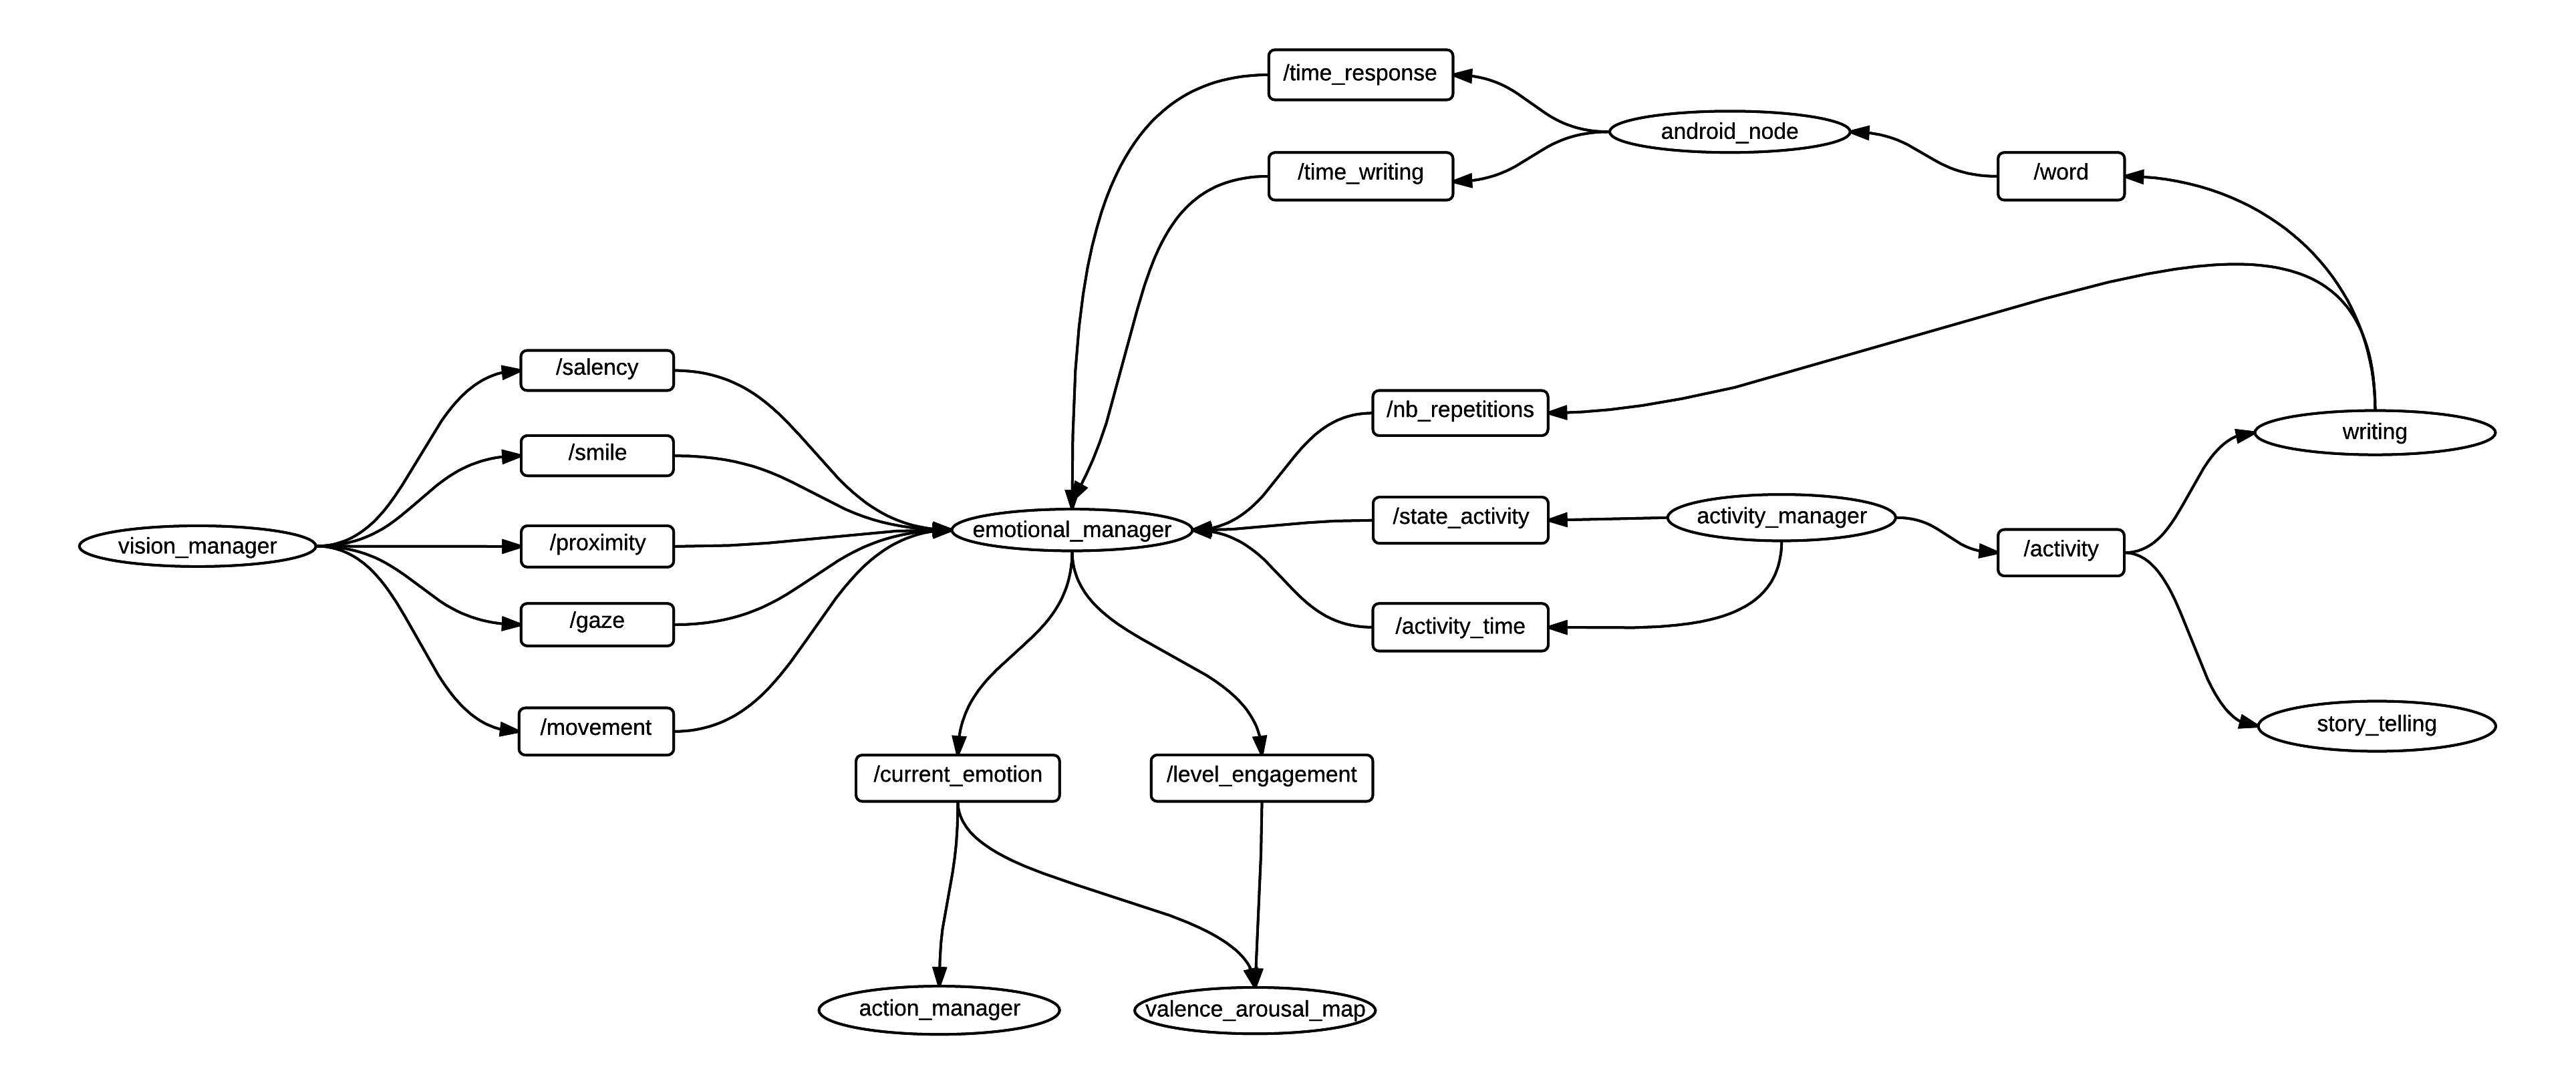
\includegraphics[scale=.57]{figures/chart.png}%     
  \end{adjustbox}
\end{figure}

\section{Vision node}
The \textit{vision} node is responsible for everything related with the features acquisition and image processing. Proximity to the robot, quantity of movement, gaze direction, smiles and saliency are the cues extracted from the scene. They will be explained in detail in the following sections. Each of them generates a 2D valence-arousal vector towards a specific behaviour.

As we previously mention, \textit{dlib} allow us to perform face pose estimation very quickly adding face landmarks to the image captured (see figure \ref{fig:dlib}).

\begin{figure}[!htb]
        \centering
        \begin{tikzpicture}[>=latex]
        	\node[inner sep=0pt] (xtion) at (0,0) {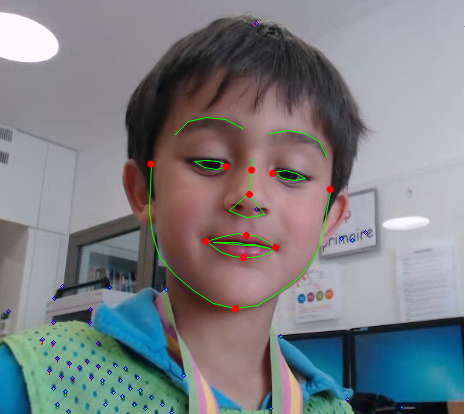
\includegraphics[width=.8\textwidth]{figures/faceMark.png}};
        	
    		\node[red, text width=1.5cm] at (-2.2,1.1) {$side_L$};
    		\node[red, text width=1.5cm] at (3.2,0.6) {$side_R$};
    		\node[red, text width=1.5cm] at (1,1.2) {$up$};
    		\node[red, text width=1.5cm] at (0,-2.7) {$chin$};
    		\node[red, text width=1.5cm] at (1.7,1.1) {$eye_R$};
    		\node[red, text width=1.5cm] at (0,1.3) {$eye_L$};
		    \node[red, text width=1.5cm] at (0.5,-0.5) {$mouth_U$};
		    \node[red, text width=1.5cm] at (0.5,-1.6) {$mouth_D$};
		    \node[red, text width=1.5cm] at (2,-1.2) {$mouth_R$};
		    \node[red, text width=1.5cm] at (-1.2,-1) {$mouth_L$};
		    \node[red, text width=1.5cm] at (1,0.5) {$nose$};
        			
       	\end{tikzpicture}
        \caption{\textit{dlib} face landmarkers in a subject experiment}
        \label{fig:dlib}
\end{figure}


\subsection{Proximity to the scene}
Back posture has been proved to be a reliable indicator of user's engagement \cite{d2007posture} \cite{castellano2009detecting}. We believe that this is directly correlated with the proximity towards the region of interaction composed, in this case, by Nao and a tablet. This can be estimated using the size of the face and it is interpreted as a positive reaction and thus, the behaviour shown is positive too (see figure \ref{fig:vaMap}). Moreover, this measurement will be recorded during the whole interaction and analysed as a possible indicator of activity engagement.

In order to be estimated, it is necessary to compute the middle point between the eyes because it decreases the variability due to the movement like in equation \ref{eq:proximity}.

\begin{equation} \label{eq:proximity}
up(x,y) = \left (\frac{eye_{L}(x)-eye_{R}(x)}{2}, \frac{eye_{L}(y)-eye_{R}(y)}{2}\right )
\end{equation}

Then, the distance in the vertical line of the face can be computed using $ up(x,y) $ and $ chin(x,y) $ as in equation \ref{eq:proximity2}:

\begin{equation} \label{eq:proximity2}
d(up,chin) = \sqrt{({(up(x)-chin(x))}^2 + {(up(y)-chin(y))}^2)}
\end{equation}

The result will induce a positive behaviour in case the child show proximity to the robot.

\subsection{Quantity of movement}
The quantity of movement, like the proximity, is captured and kept during the interaction. However, as happens with the proximity, it is also useful to model behaviour responses with Nao. In order, to catch the movement from the scene, several methods were tested. We selected a method based on optical-flow since it is less sensitive to image noise than point-wise methods.

The algorithm finds the most prominent corners in the image computing the corner Minimum Eigenvalue as described in \cite{shi1994good}, which stores the minimal eigenvalue of a block size neighbourhood \textit{S(p)}, that is, $ \min(\lambda_1, \lambda_2) $ in terms of the following equation:

\begin{equation}
M =  \begin{bmatrix} 
		\sum _{S(p)}(dI/dx)^2 &  \sum _{S(p)}(dI/dx dI/dy)^2  \\ 
		\sum _{S(p)}(dI/dx dI/dy)^2 &  \sum _{S(p)}(dI/dy)^2 
	 \end{bmatrix}
\end{equation} 

where the derivatives are computed using the \textit{Sobel} operator. After that, it finds the minimum eigenvalue of \textit{M} and stores them.

Once the relevant points are detected, the second step is to calculate the flow from these points. The technique used is based on Lucas-Kanade method with pyramids implemented in OpenCV \cite{bouguet2001pyramidal} which assumes that the flow is essentially constant in a local neighbourhood of the pixel under consideration and solves the basic optical flow equations for all the pixels in that neighbourhood by the least squares criterion. Being the equations formulated as in \ref{lucasKanade}.

\begin{equation} \label{lucasKanade}
A =  \left( \begin{array}{cc}
	I_x(q_1) & I_x(q_1) \\
	I_x(q_1) & I_x(q_1) \\
	\colon & \colon  \\
	I_x(q_n) & I_x(q_n)
	\end{array} \right),
\qquad  
v =  \left( \begin{array}{cc}
		V_x  \\
		V_y \\
	\end{array} \right),
\qquad	 	 
b =  \left( \begin{array}{c}
	 		-I_t(q_1)\\
	 		-I_t(q_2)\\
	 		\colon \\
	 		-I_t(q_n)\\
	 \end{array} \right)
\end{equation}

This system has more equations than unknowns and thus it is usually over-determined. So, needs to be reformulated as shown in \ref{lucasKanade1}. 

\begin{equation} \label{lucasKanade1}
A^TAv = A^Tb
\qquad
\Rightarrow
\qquad
v=(A^TA)^{-1}A^Tb
\end{equation}

In the final analysis, the result can be seen in figure \ref{fig:optical}. In this case the high quantity of movement is interpreted as a negative input inducing an angry behaviour.

\begin{figure}[h!]
        \centering
        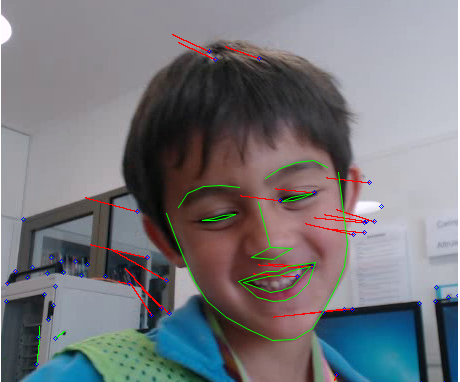
\includegraphics[width=0.5\textwidth]{figures/optical.png}
        \caption{Optical flow output in a real interaction context}
        \label{fig:optical}
\end{figure}

\subsection{Gaze direction}
The gaze direction was computed using a simple but effective method through the landmark positions provided by the face pose estimation. As it happens with the quantity of movement, as well as with the proximity, the data acquired is interpreted for both, behaviour adaptation and engagement assessment.

First, we compute the length of the segments between the right and the left face sides ($ side_R $ and $ side_L $, respectively) with respect to the nose, $ d(nose,side_R) $ and $ d(nose,side_L) $, as well as the distance between both sides, $ d(side_R,side_L) $. So, it results in equation \ref{eq:estwest},

\begin{equation} \label{eq:estwest}
horizontal = \frac{d(nose,side_R)-d(nose,side_L)}{d(side_R,side_L)}
\end{equation}

where the result is normalized in the range $ [-1,1] $. A value greater than a threshold of 0.3 indicates \textit{left} as gaze direction, whereas lower than -0.3 indicates \textit{right} direction.

Second, we perform a similar operation to detect when a user is looking up or down. It is necessary to calculate the projection of the nose position in the \textit{horizontal} segment that goes from $ side_R $ to $side_L$ like in equations \ref{eq:projection} and \ref{eq:projection1}.

\begin{equation}\label{eq:projection}
d_{proj} = d(nose,side_R) \cdot \left(\frac{horizontal}{d(nose,side_R)} + d(nose,side_L)\right )
\end{equation}

\begin{equation} \label{eq:projection1}
proj(x,y) = \frac{P_{side_R}(x,y)+(P_{side_L}(x,y)-P_{side_R}(x,y))\cdot d_{proj}}{horizontal}
\end{equation}

Then, we can compare if the height of $ proj(x,y) $ is greater or lower than the nose position with a certain tolerance. If it is the case, the user is looking up or down respectively. Finally, if none of the directions is satisfied, we assume that the user is looking straight at the robot inducing a positive behaviour.


\subsection{Saliency}

The \textit{saliency} is a concept that is related with the changes on the current state of the scene. Events such as a new person detected in the scene as well as quick movements after a period of tranquility or vice-versa, are considered as a novelty. It can be used to modify the current status of the robot towards a \textit{surprise} behaviour.

The algorithm implemented for this detection consist on the Exponential Moving Average (EMA), defined in equation \ref{eq:EMA},

\begin{equation} \label{eq:EMA}
 t > 1,\ \    S_{t} = \alpha \cdot Y_{t} + (1-\alpha) \cdot S_{t-1}
\end{equation}

where,

\begin{itemize}
\item The coefficient $ \alpha $ represents the degree of weighting decrease, a constant smoothing factor between 0 and 1. A higher $ \alpha $ discounts older observations faster.
\item $ Y_t $ is the value at a time period \textit{t}.
\item $ S_t $ is the value of the EMA at any time period \textit{t}.
\end{itemize}

Once the EMA $S_t$ value is computed, the distance with respect to the previous EMA, $S_{t-1}$ needs to be computed of course, for each kind of event (gaze, proximity...), as shown in equation \ref{eq:EMA2}.

\begin{equation} \label{eq:EMA2}
d = \frac{(S_t - S_{t-1})^2}{\epsilon + (S_t + S_{t-1})^2 }
\end{equation}

When a high quantity of movement is captured after a period without movement, a new face is detected, or the proximity changes in great manner, it produces a behaviour response in the field of surprise.

\subsection{Child smiles}
In order to capture the smile of the children, it has been necessary to calculate the intersection between the segment composed by the two mouth corners, $ mouth_L $ and $ mouth_R $, and the vertical ones, $mouth_U$ and $mouth_D$. Whenever there is no intersection is due to a smile: The segment composed by $mouth_U$ and $mouth_D$ is above the $mouth_U$ point. However, the detections are restricted to the robot eye contact situations only, helping to induce a happy behaviour.


\section{Emotion manager node}
This node is responsible for the vectorization of the incoming information from the \textit{vision} node and eventually, the computation of the correspondent valence and arousal values. Furthermore, besides the features extracted from the \textit{vision} module, there are additional ones such as; the time spend in the activity or the number of repetitions that have an influence in the resulting vectorization of the current state (see figure \ref{fig:vectMap}). The summary of the cues used, the direction of the correspondent vectors (valence, arousal) assuming an initial point $ (0,0) $, the weight of them in the final computation, as well as the cues that are used for the engagement assessment are shown in table \ref{tab:cues}.

\begin{table}[h!]
\centering
\begin{tabular}{l|l|l|l|l}
 \textbf{Features}   & \textbf{Valence}  & \textbf{Arousal}  & \textbf{Weight} & \textbf{Engagement}\\ \hline	
 \textit{QoM}  	  		  	 &   -1 	      	 &    1 	& 14\% &   +  \\ \hline
 \textit{Proximity}    	  	 &   1  	      	 &    1		& 7\%  &   +  \\ \hline
 \textit{Saliency}	  	  	 &   0 	      		 &    1 	& 7\%  &   +  \\ \hline
 \textit{Gaze: robot contact} 	 &   1	      	 &    1 	& 5\%  &   +  \\ \hline
 \textit{Gaze: left, right, up, down} & -1	     &   -1     & 5\%  &   +  \\ \hline
 \textit{Smiling}	  	  	 &   1 	      		 &    1 	& 60\% &      \\ \hline
 \textit{Time activity}	  	 &   -1	      		 &   -1 	& 1\%  &      \\ \hline
 \textit{Number repetitions} &   -1 	         &   -1	    & 1\%  &       	

\end{tabular}
\caption{Summary of the features in valence, arousal, weight and engagement assessment}
\end{table}\label{tab:cues}

 \begin{figure}[!htb]
	\centering
	\begin{tikzpicture}[>=latex]

		\node[inner sep=0pt] (xtion) at (0,0) {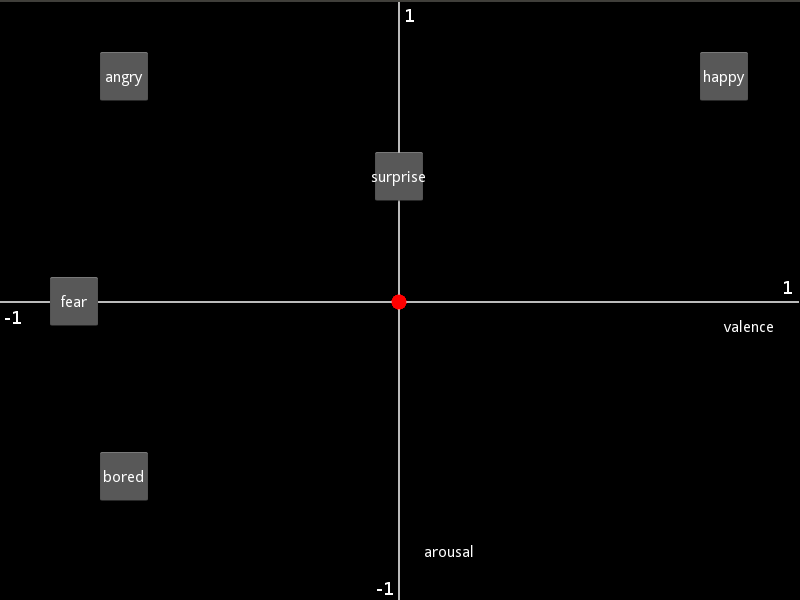
\includegraphics[width=.8\textwidth]{figures/vectMap.png}};

		\draw[->, color=green, thick] (0,0) -- (2,1.5);
		\draw[->, color=yellow, thick] (0,0) -- (0,1.2);
		\draw[->, color=blue, thick] (0,0) -- (-1.5,-1);
		\draw[->, color=red, thick] (0,0) -- (-1,0.75);
		\draw[red,fill=red] (0,0) circle (.8ex);
		
		\draw[white, thick,dashed] (0,3.5) ellipse (1cm and 0.5cm);
		\node[white, text width=2cm] at (0.6,3.45) {\tiny
		Saliency
		};
		
		\draw[white, thick,dashed] (-2,-2.5) ellipse (1.5cm and 1cm);
		\node[white, text width=2.5cm] at (-1.7,-2.5) {\tiny
		Time activity
		
		Number repetitions
		Ignoring
		};
		
		\draw[white, thick,dashed] (3.5,2) ellipse (1.5cm and 1cm);
		\node[white, text width=1.5cm] at (3.7,2) {\tiny
		Smiling
		
		Eye contact		
		Proximity
		};
		
		\draw[white, thick,dashed] (-2.4,2.5) ellipse (1cm and 0.5cm);
		\node[white, text width=2cm] at (-2,2.45) {\tiny		
		High QoM	
		};
	\end{tikzpicture}
    \caption{Valence and arousal map with all features compressed between -1 and 1}
    \label{fig:vectMap}
\end{figure}

\subsection{Direction and weighting}
The direction of the marker that defines the current behaviour (see red dot in figure \ref{fig:vectMap}) depends on the fusion of all different features with their respective weights. The formula that computes the resulting valence and arousal values provided to the action node is shown in \ref{eq:weight}.

\begin{equation}
 \vec{P_{t}}(val,aro) = \sum_{i=1}^N\vec{F}_{i}(val,aro) \cdot w_i
\end{equation}\label{eq:weight}

where $\vec{P_{t}}(val,aro)$ is the vector that defines the behaviour at time \textit{t} encoded by valence and arousal values. It is based on the combination of all vector features $ \vec{F}_{i} $ multiplied by their respective weights \textit{w}.

\section{Action node}
Finally, this node is the interface with the robot actuators. This node has been designed to encode all resources shown in the list located in section \ref{listResources} into the map shown in figure \ref{fig:vectMap}.

In the case of the physical joints, they are distributed uniformly along the map taking into account the limitations of the joint angles. For instance, the behaviour that corresponds to the point \textit{(0.8,0.8)} in the valence/arousal map in figure \ref{fig:vectMap} would not only move the arms, showing a positive expression, but also the head in a upper position among others.

In this way, the result received from the \textit{emotion manager} node with range $ [-1,1] $ is used to access the correspondent position stored in a matrix (for LEDs, pitch and volume) as well as used to modify the available joints for a certain duration of time. For instance, the shoulder roll, both right and left, are constrained between $ -76\degree $ and $ 18\degree $ were the values are defined by the \textit{valence} multiplied by a certain scale factor. The different actuators depend directly on the valence-arousal values as follows: 

\begin{itemize}
\item Head pitch: The head position of the robot is influenced exclusively by the arousal value. The higher the value, the higher the head position.

\begin{figure}[h!]
        \centering
        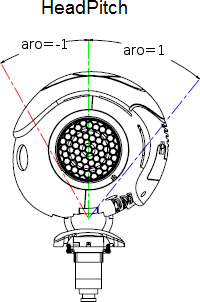
\includegraphics[width=0.2\textwidth]{figures/head.png}
        \caption{Head pitch boundaries for valence and arousal \cite{aldebaran}.}
        \label{fig:head}
\end{figure}

\item Shoulders pitch and roll: Shoulders have a pitch of +2 to -2 radians. Used in absolute mode, the central pitch value is 1.4 radians. It is exclusively modified by the valence value.

\begin{figure}[h!]
        \centering
        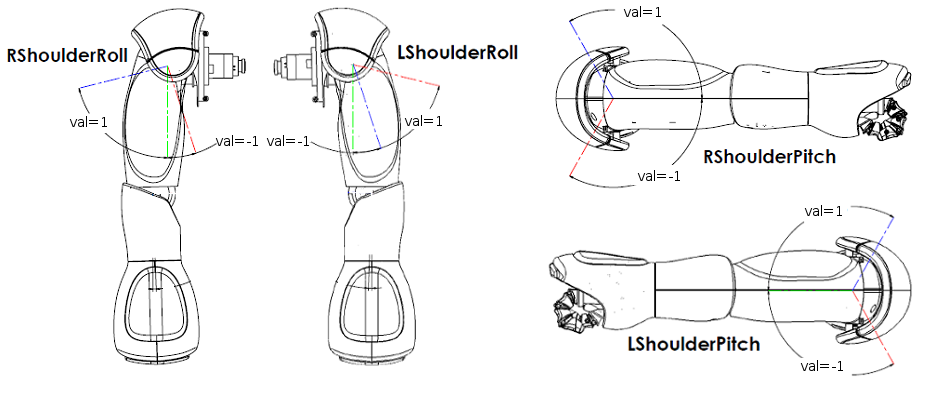
\includegraphics[width=0.8\textwidth]{figures/parts.png}
        \caption{Shoulder pitch and roll boundaries \cite{aldebaran} for valence and arousal.}
        \label{fig:parts}
\end{figure}

\item Pitch and volume: A matrix of 11x11 tuples was designed to keep the information of both pitch and volume. In this case, this feature is only modified by a the arousal value since the fundamental frequency of voice, speech rate and speech volume of the voice all seem to be related to the arousal of the emotion felt \cite{banse1996acoustic}. The values are integers of range $ [-1,1] $. 
\item LEDs: The same kind of matrix (in hexadecimal) was used to modify the eye colors. An example can be found in matrix \ref{eq:matrices}. In this case too, the color is defined by an arousal value since red colours are associated with high arousal emotions whereas blue ones with low arousal \cite{elliot2014color}.

\vspace{0.5cm}

\end{itemize}
\begin{equation}\label{eq:matrices}
M =  \begin{bmatrix} 
		\textcolor{red}{0xF82C35} & \textcolor{red}{0xF82C35} & \textcolor{RedOrange}{0xD55528} & \textcolor{RedOrange}{0xD55528} & ... & \textcolor{green}{0x56C427}  \\
		\textcolor{red}{0xF82C35} & \textcolor{red}{0xF82C35} & \textcolor{BurntOrange}{0xD5542A} & \textcolor{BurntOrange}{0xD5542A} & ... & \textcolor{ForestGreen}{0x56C427}  \\
		\textcolor{BrickRed}{0xF62D35} & \textcolor{BrickRed}{0xF62D35} & \textcolor{BrickRed}{0xF62D35} & \textcolor{Bittersweet}{0xE96A37} & ... & \textcolor{JungleGreen}{0x56C427}  \\
			:	 &	:		&		:  &		: & :   & 		: 	  \\
		\textcolor{Fuchsia}{0x692850} & \textcolor{Fuchsia}{0x692850} & \textcolor{Fuchsia}{0x692850} & \textcolor{Fuchsia}{0x692850} & ... & \textcolor{MidnightBlue}{0x0085BE}		
	 \end{bmatrix}_{11x11}
\end{equation}

\vspace{0.5cm}

It is important to notice that not all feature actions are executed continuously during the activities. This is the case only of the volume and pitch and the color changing. The rest of the movements are performed in specific times to avoid collisions with the current activity, for instance, the arm movement in the writing process  Most of them are applied during the \textit{waiting for feedback} state shown in figure \ref{fig:stateMachine}. Furthermore, a face tracking is performed continuously in order to provide eye contact with the user, using \textit{ALFaceDetection} from NaoQi, which is based on a commercial face detection solution.

\section{Results}
The result of the adaptive behaviour model \footnote{https://github.com/chili-epfl/emotional-manager} is shown in figure \ref{fig:behaviours}. 

\begin{figure}[h!]
        \centering        
        \begin{subfigure}[b]{0.18\textwidth}
                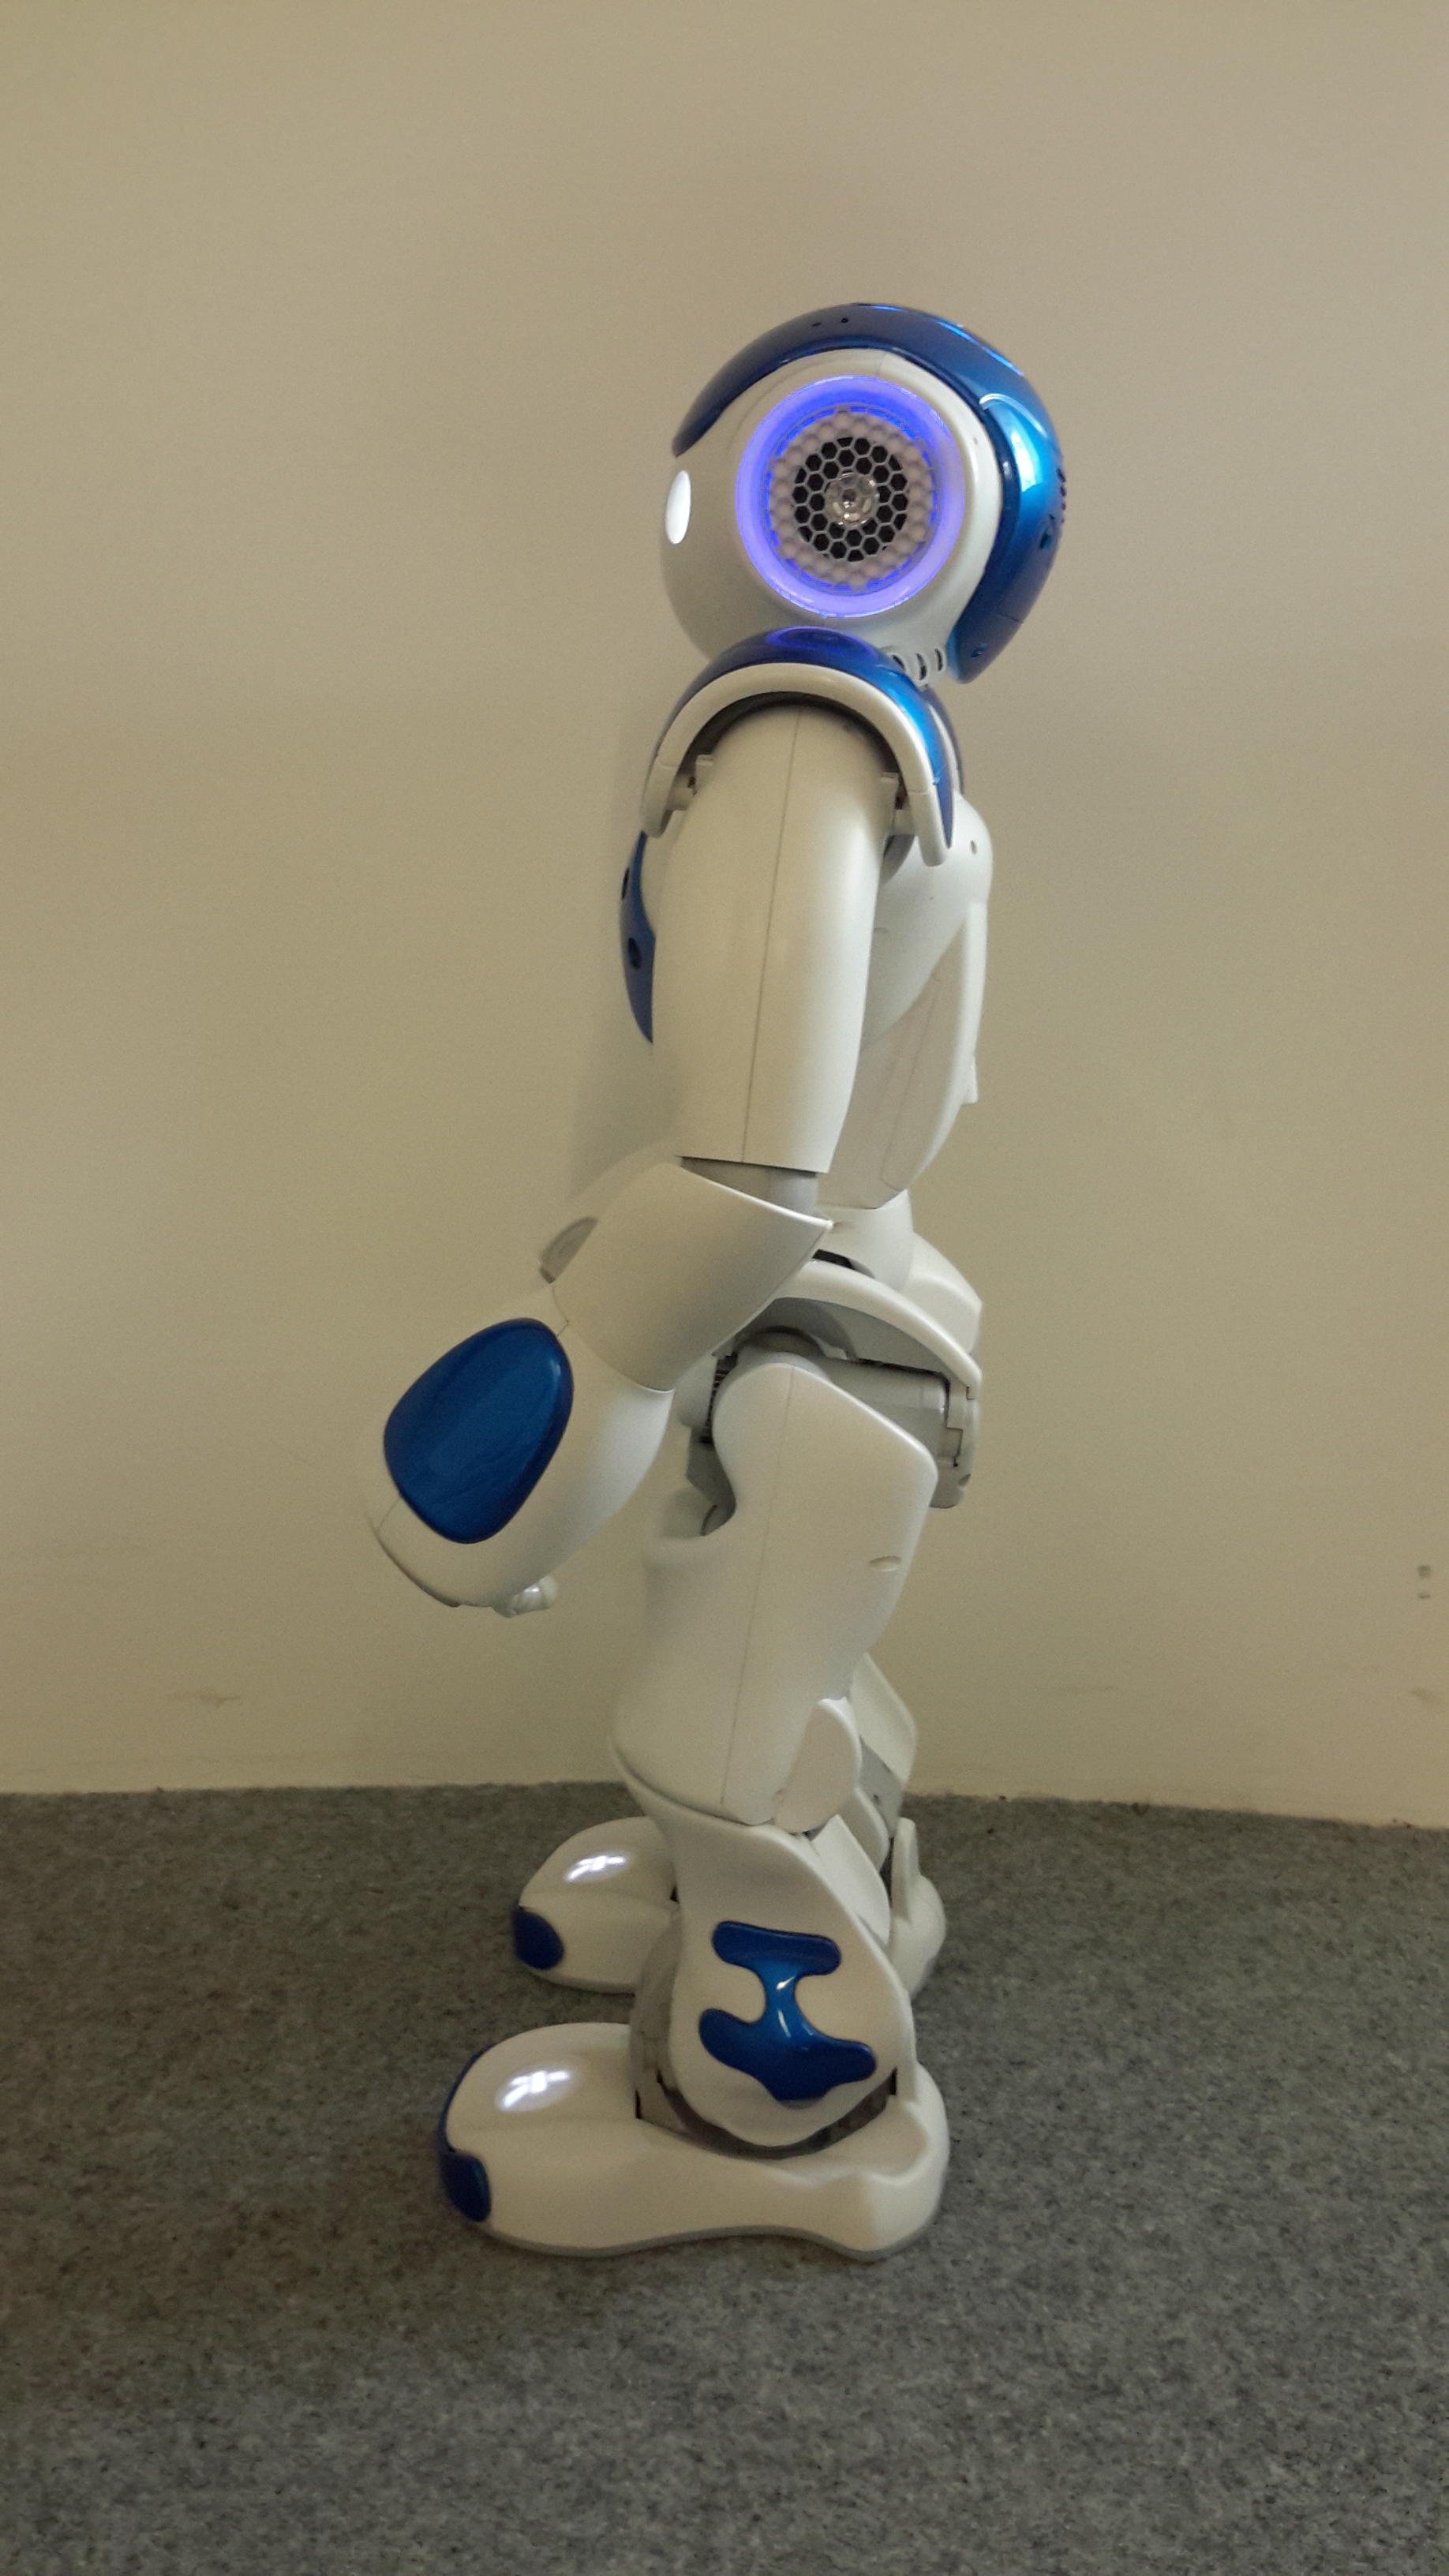
\includegraphics[width=\textwidth]{figures/neutral.jpg}
                \caption{Neutral}
                \label{fig:neutral}
        \end{subfigure}
        ~ %add desired spacing between images, e. g. ~, \quad, \qquad, \hfill etc.
          %(or a blank line to force the subfigure onto a new line)
        \begin{subfigure}[b]{0.18\textwidth}
                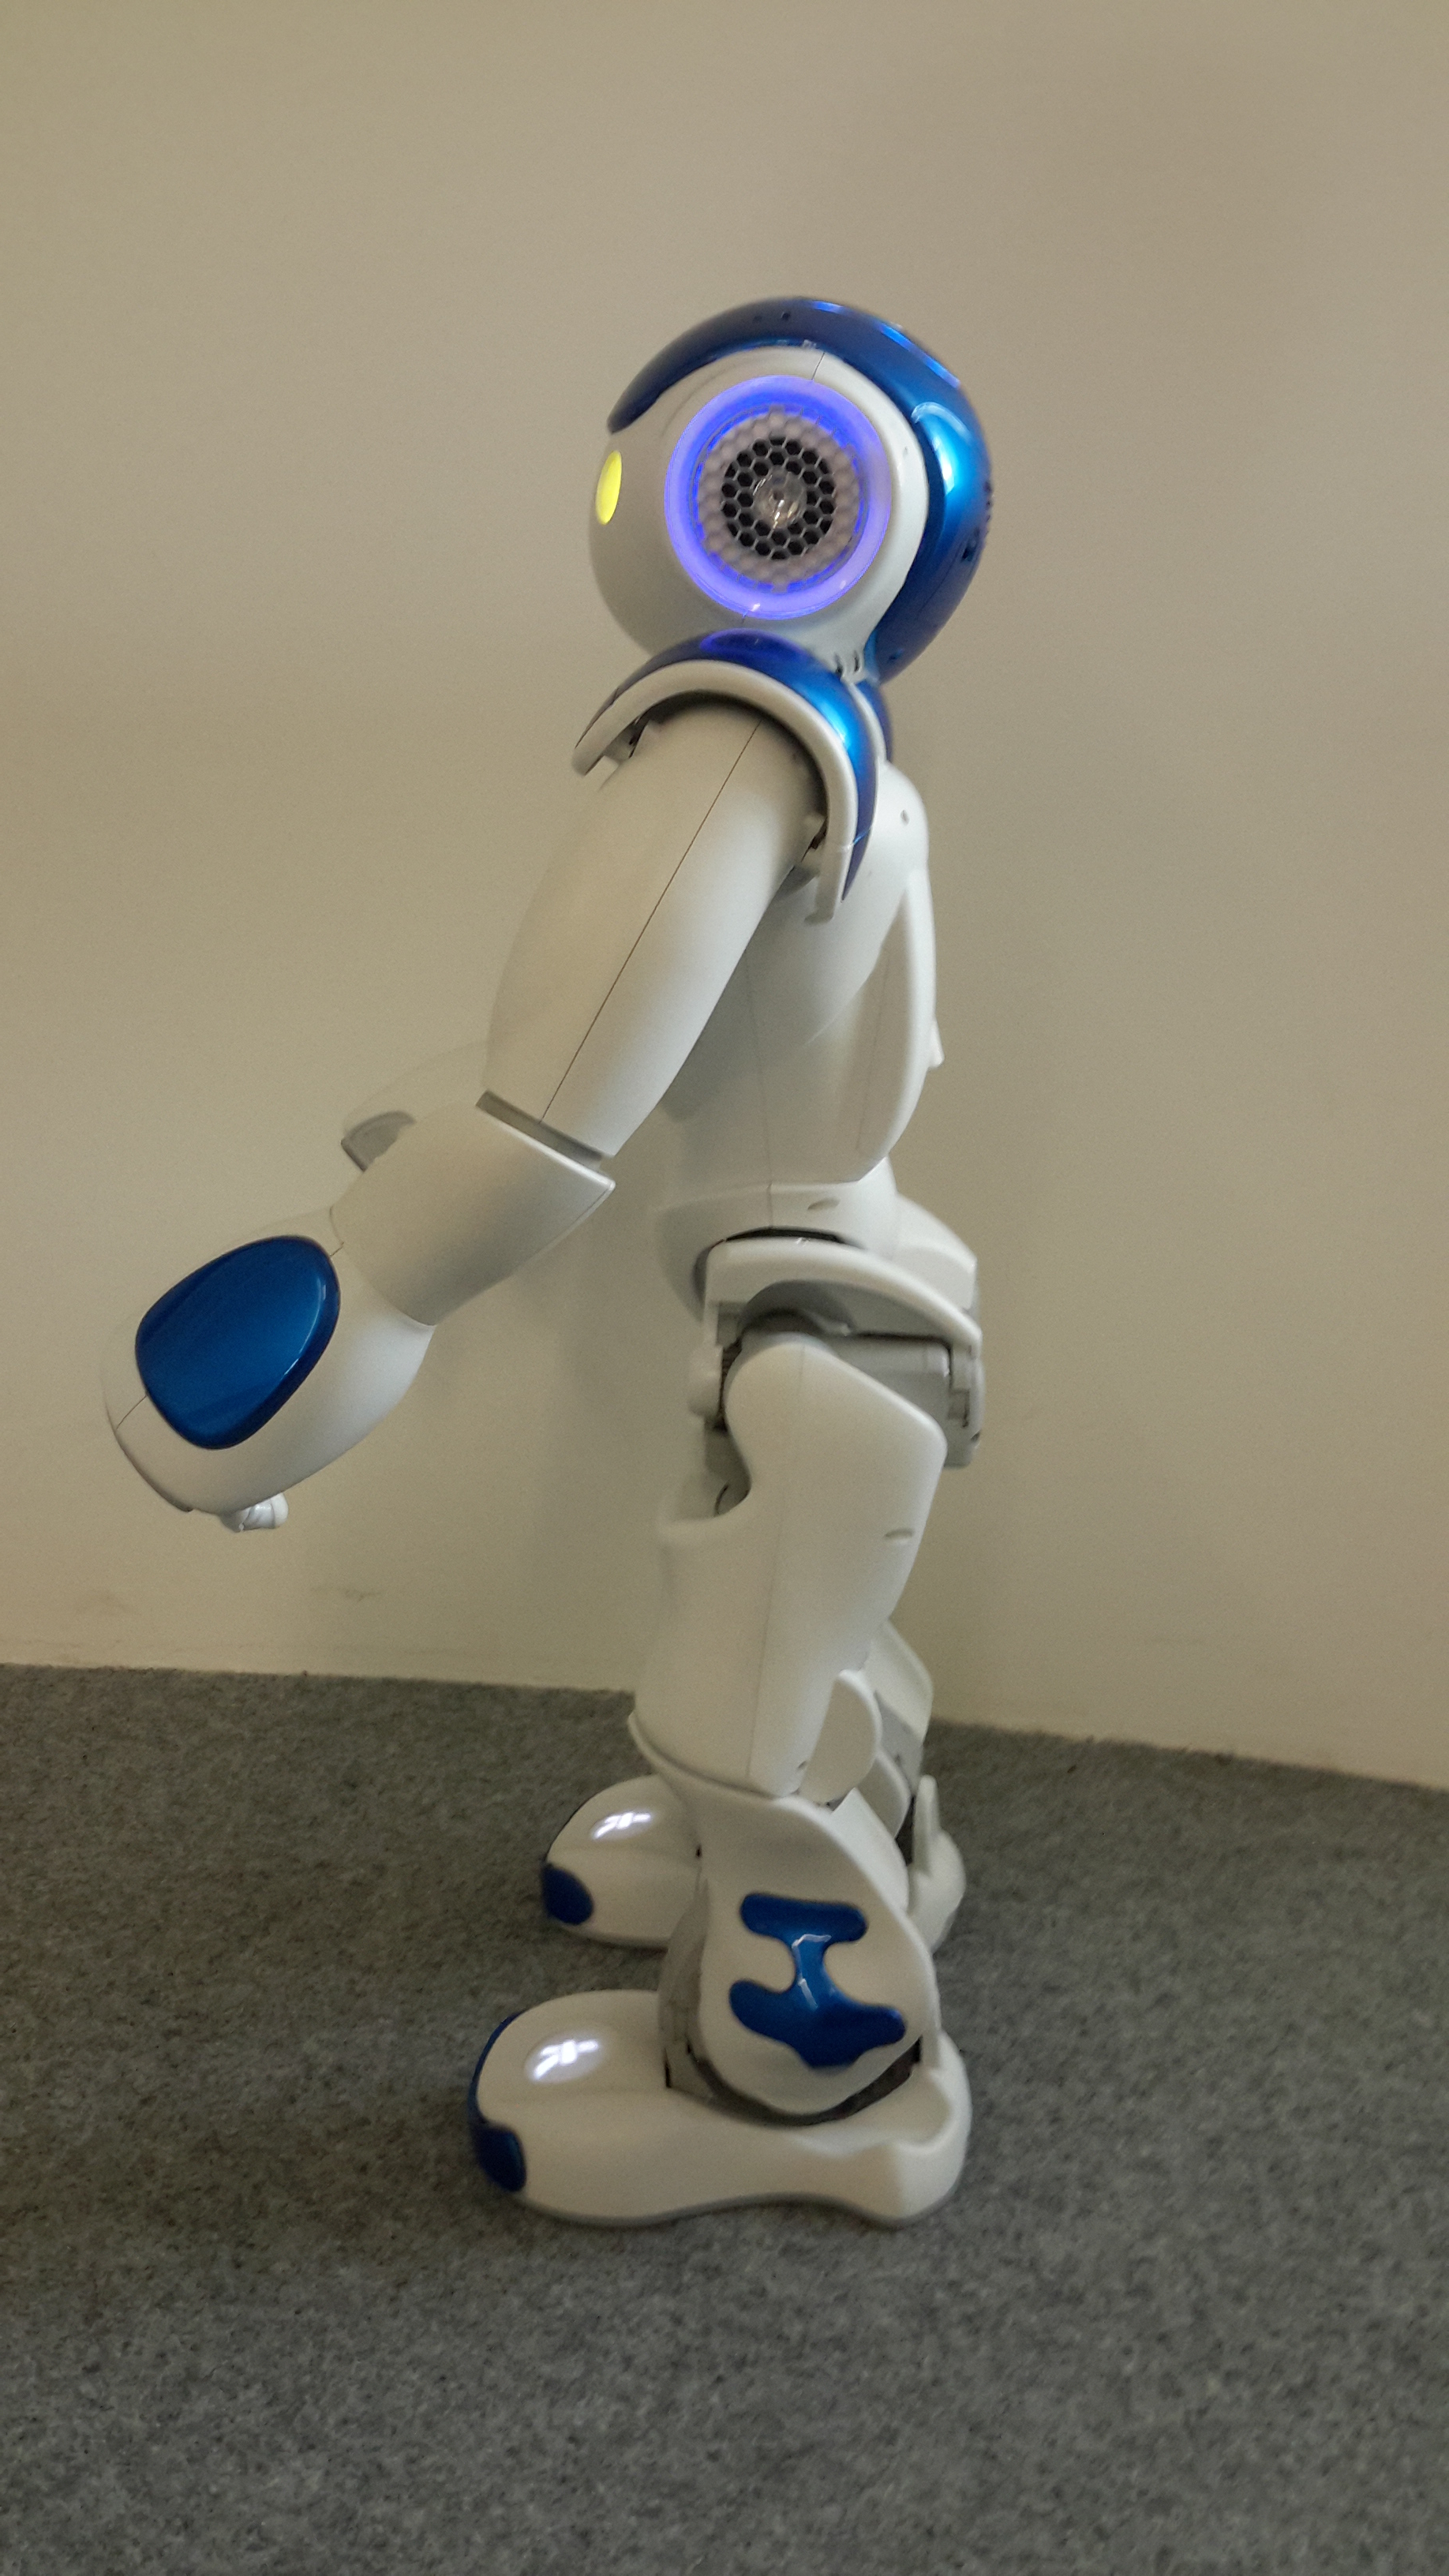
\includegraphics[width=\textwidth]{figures/happy.jpg}
                \caption{Happy}
                \label{fig:happy}
        \end{subfigure}%
        ~ %add desired spacing between images, e. g. ~, \quad, \qquad, \hfill etc.
          %(or a blank line to force the subfigure onto a new line)
        \begin{subfigure}[b]{0.18\textwidth}
                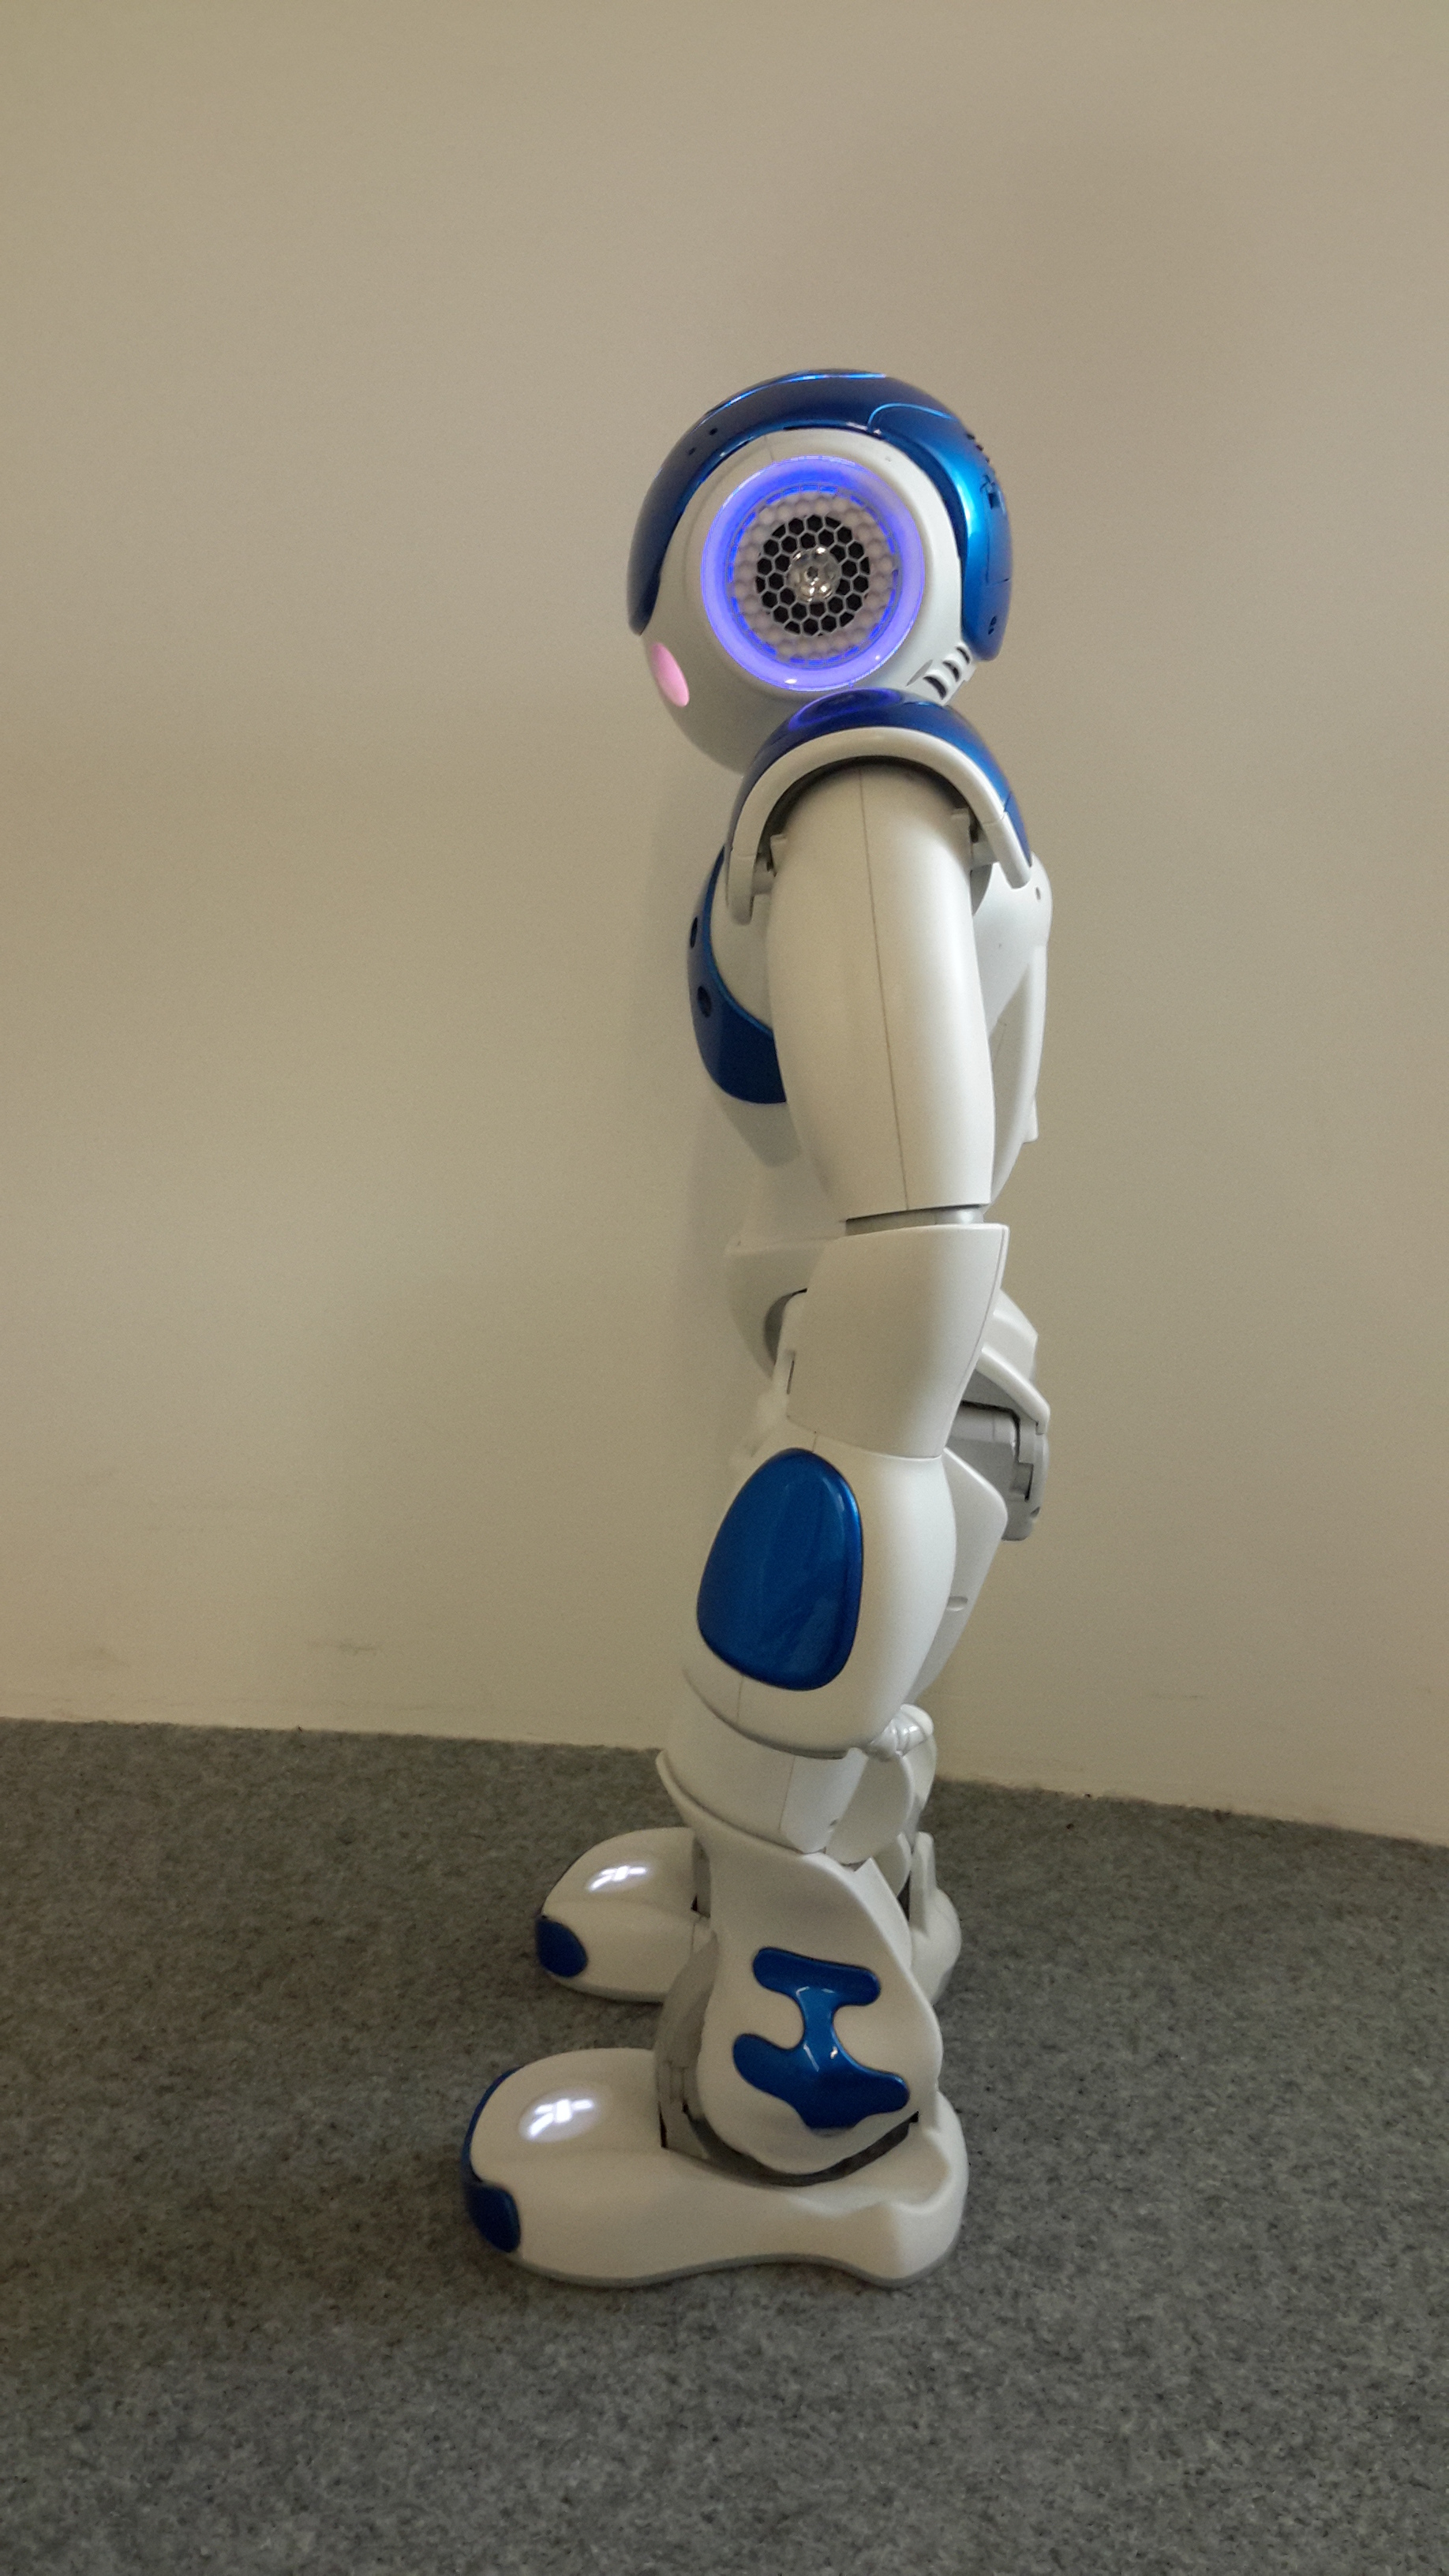
\includegraphics[width=\textwidth]{figures/sad.jpg}
                \caption{Sad}
                \label{fig:sad}
        \end{subfigure}
        ~ %add desired spacing between images, e. g. ~, \quad, \qquad, \hfill etc.
          %(or a blank line to force the subfigure onto a new line)
        \begin{subfigure}[b]{0.18\textwidth}
                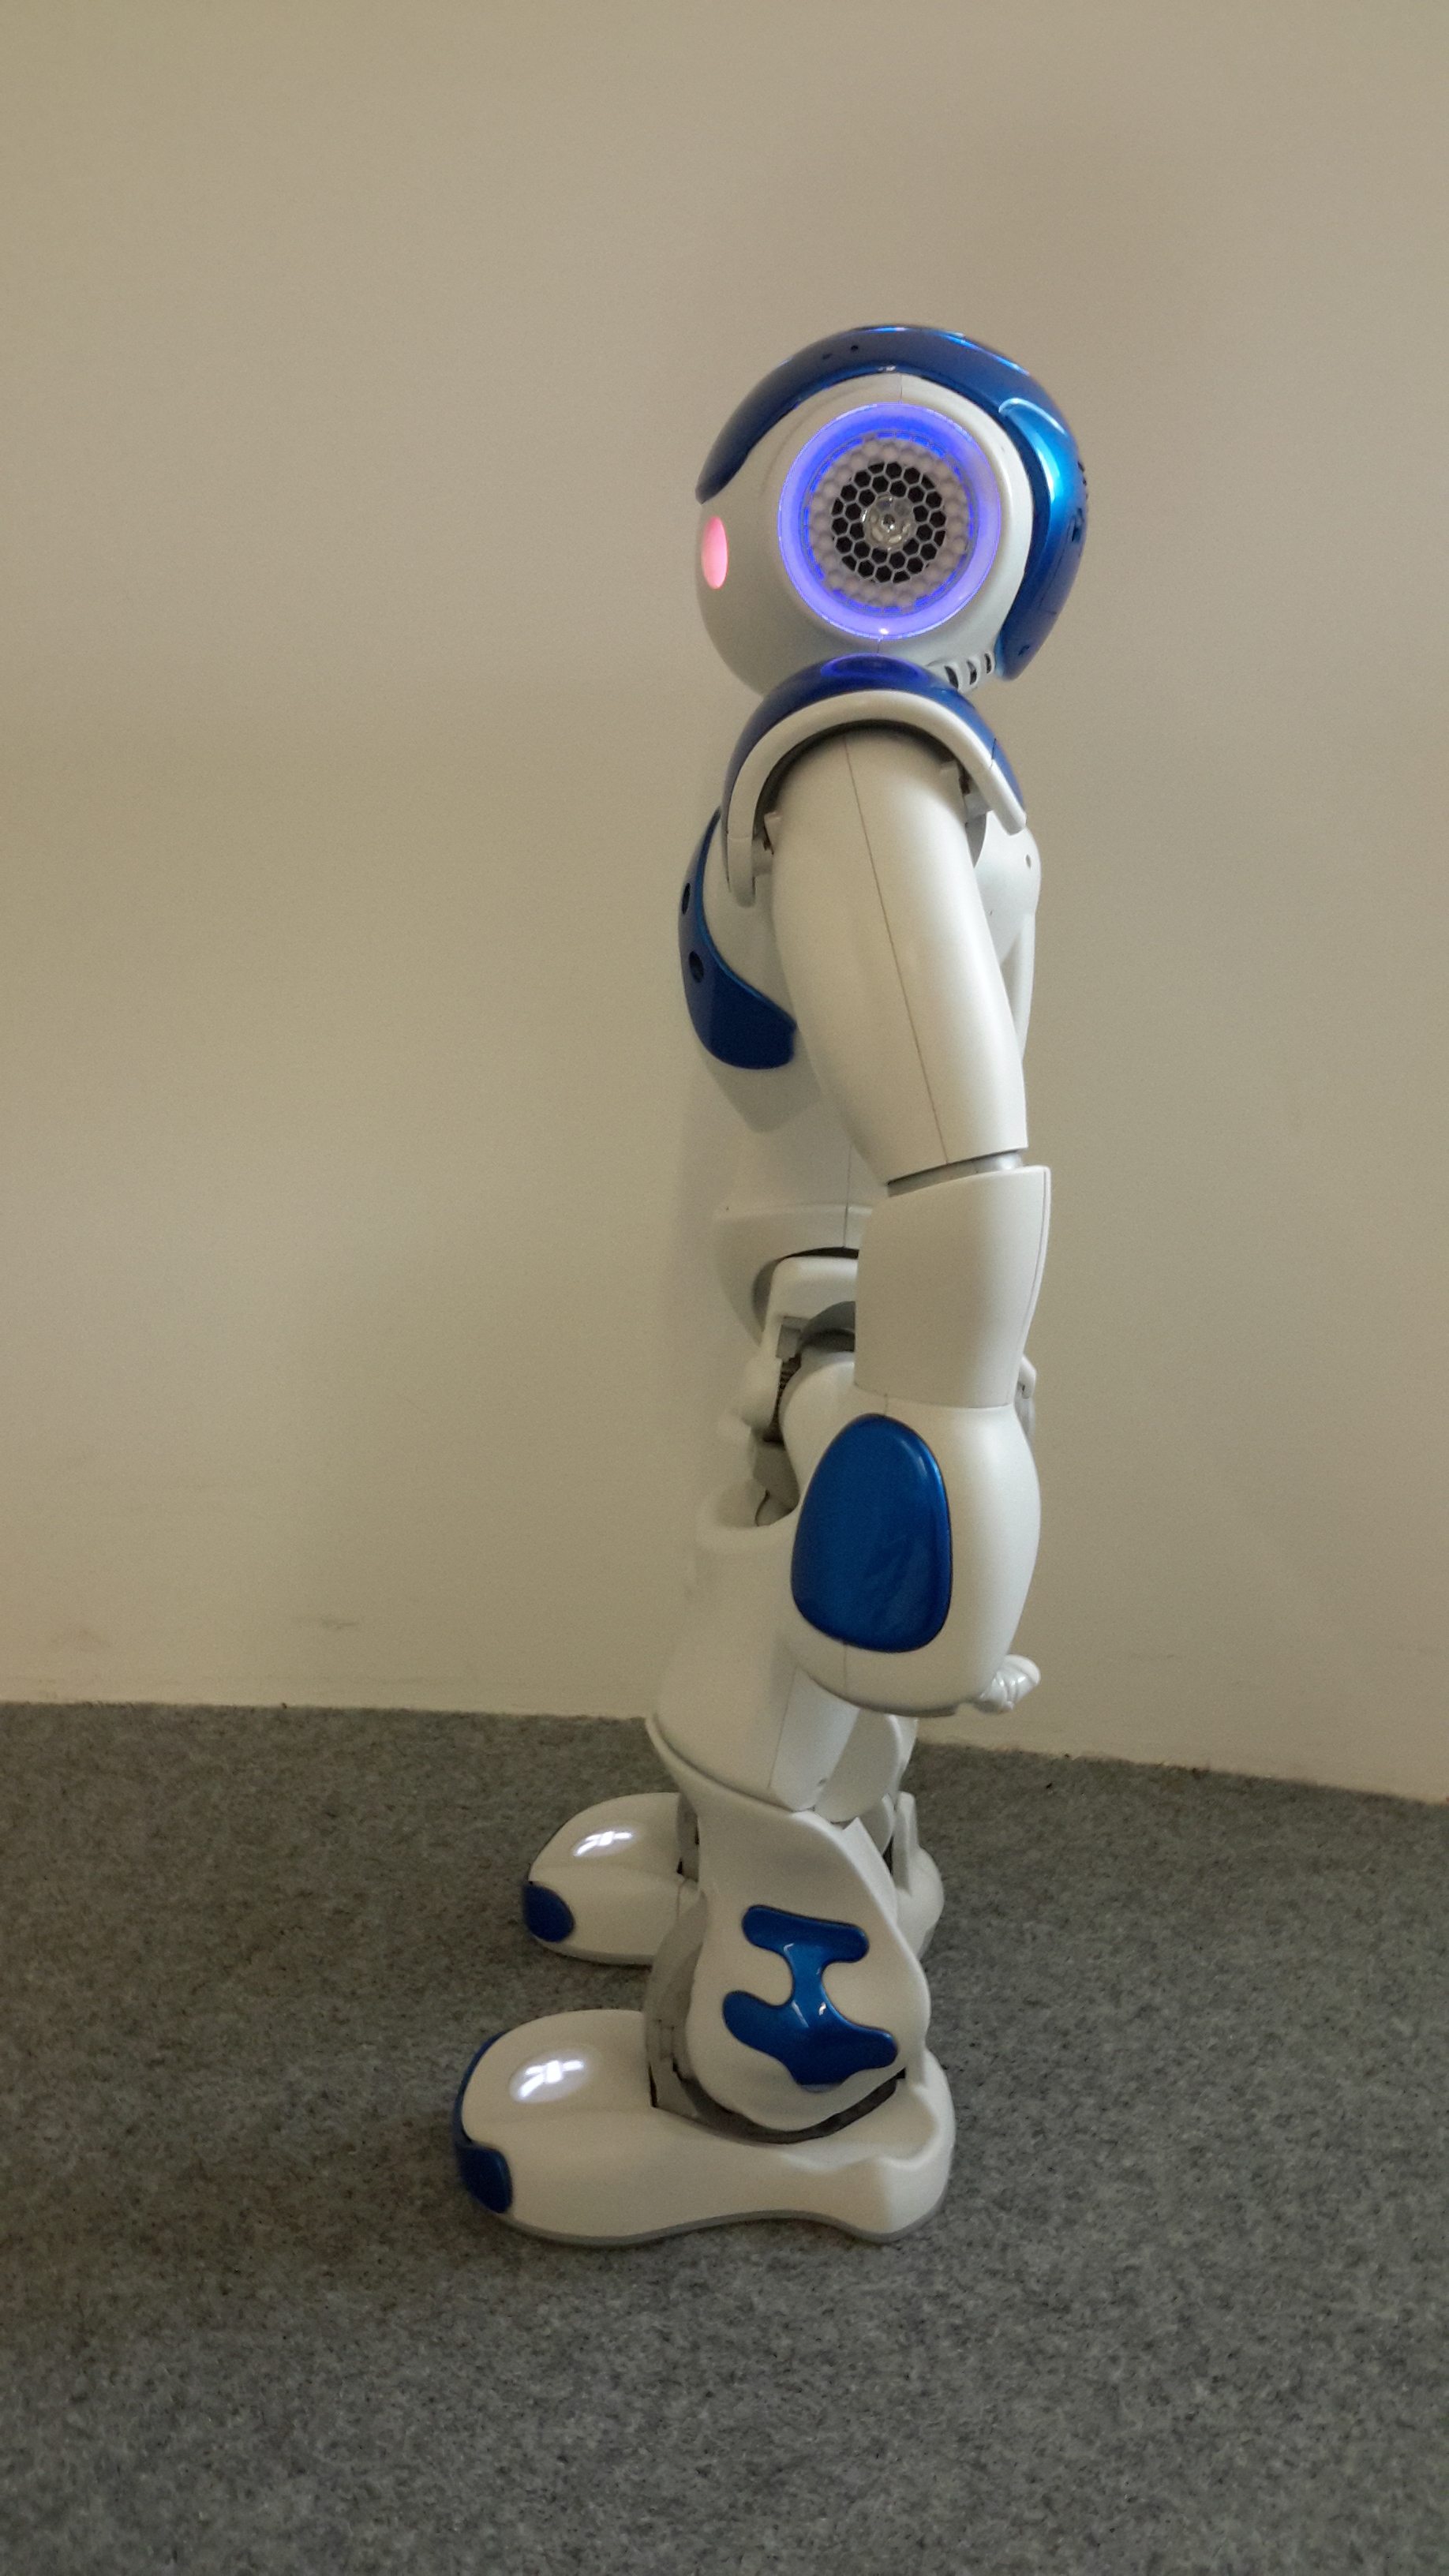
\includegraphics[width=\textwidth]{figures/bored.jpg}
                \caption{Bored}
                \label{fig:bored}
        \end{subfigure}
        ~ %add desired spacing between images, e. g. ~, \quad, \qquad, \hfill etc.
          %(or a blank line to force the subfigure onto a new line)
        \begin{subfigure}[b]{0.18\textwidth}
                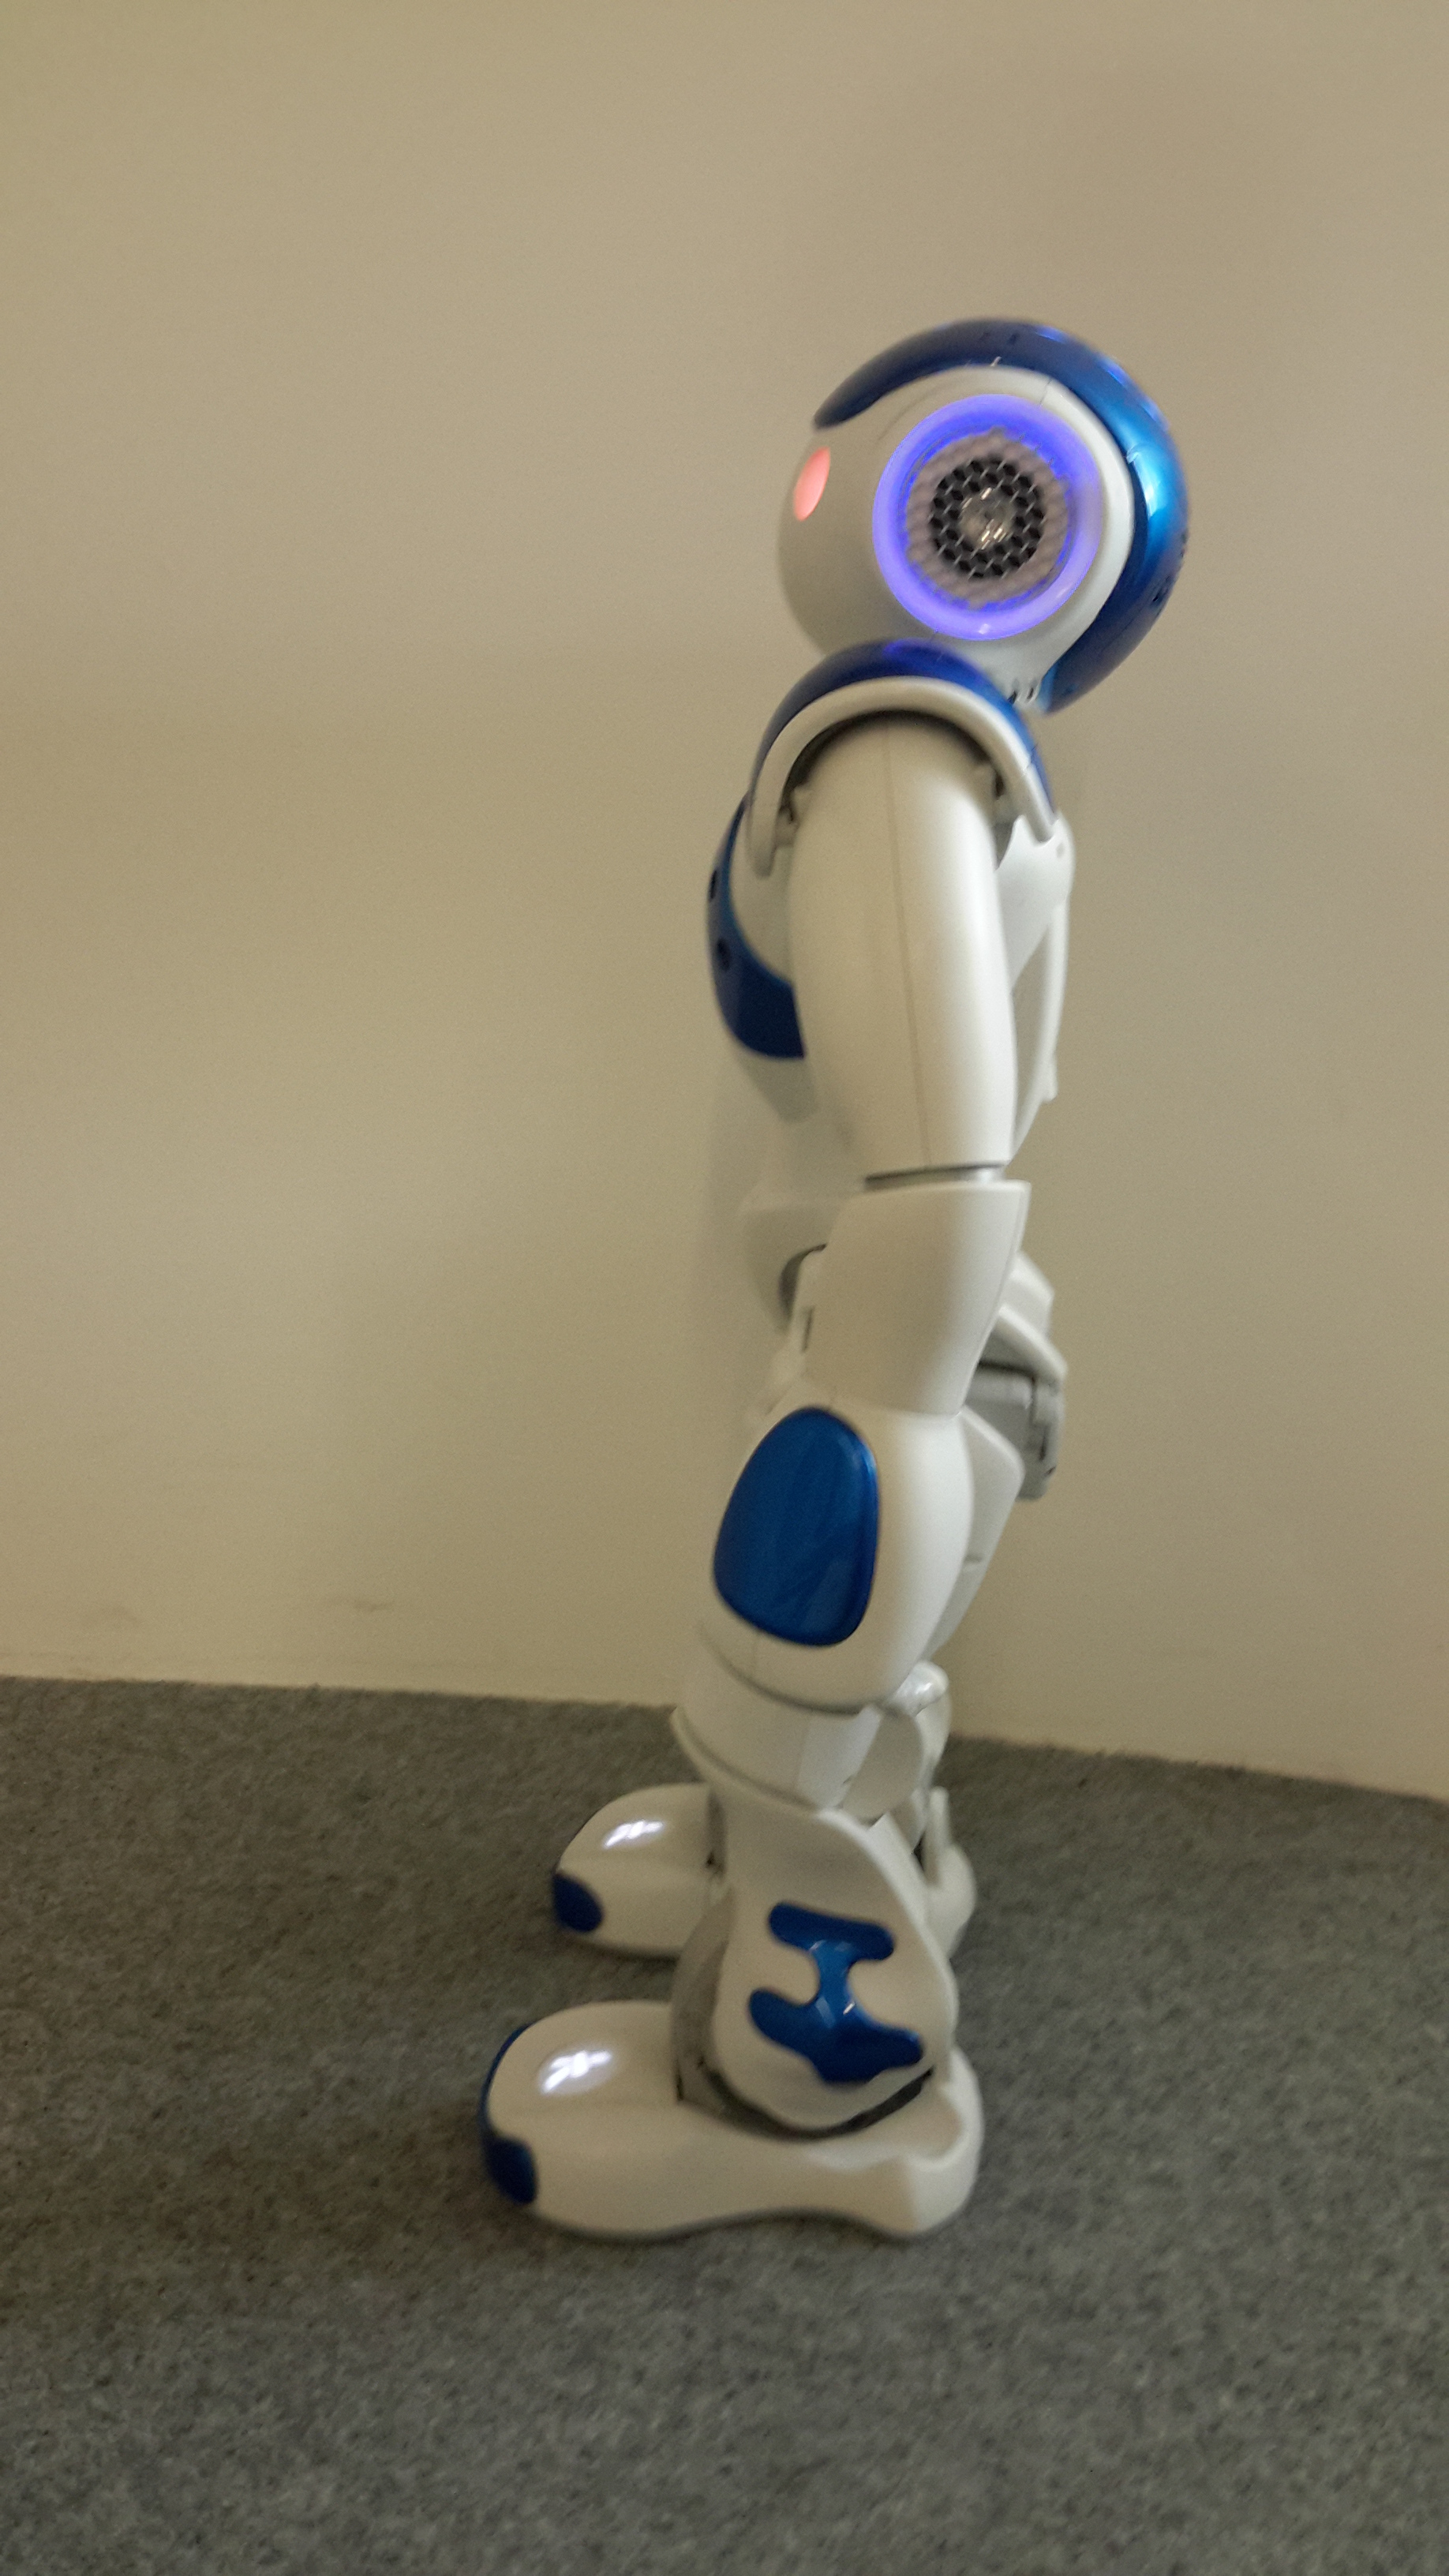
\includegraphics[width=\textwidth]{figures/angry.jpg}
                \caption{Angry}
                \label{fig:angry}
        \end{subfigure}
		\caption{Examples of behaviours generated by the valence-arousal model}\label{fig:behaviours}
\end{figure}

\chapter{Experiments} \label{chap:feasibility}

In this chapter two experiences in the field and the procedure followed in each case are reported. A feasibility study is introduced first in section \ref{sec:feasibility} and next, the real experiments for data acquisition are reported in section \ref{sec:experiment}.

\section{Feasibility study with children}\label{sec:feasibility}
It is imperative that a system which is ultimately to be used with children is tested in the hands
of children as soon as possible, to promote development of the design in the most appropriate
and necessary directions. To this end, a feasibility study was planned at a school on 30th of April
2015.

\subsection{Expected outcomes}

The desired outcome is the collection of all relevant information related with the robustness of the system and the experiment protocol, including

\begin{itemize}
\item the proper detection of the most relevant features captured to assess a measurement of the level of engagement and,
\item the implementation of an activity framework for easy addition of new activities.
\end{itemize}

This study should also allow the acquisition of a ground truth model of engagement using the manual assessment by two human observers during the interaction given an established criteria.

\subsection{Implementation of the activity framework}
The implementation has been split into two different ROS packages; the first one involves the management of activities. An activity can be writing (original CoWriter) or a simple story telling. And the second one, the adapting model behavior called \textit{emotionManager}. The execution of this second package is designed in such a way that becomes totally independent from the activities, and acts instead as a modifier inserting behaviors along the interaction. It is explained in detail in chapter \ref{chap:systemOverview}.

Following from previous tests conducted in the laboratory, a need for a higher level management of the interaction in the software was identified. Specifically, the need to control efficiently several activities and allowing it from external packages such as the emotion manager.

In order to reach this goal, the previous version of the state machine implemented to model the interaction \cite{hood2015children} was modified and extended to allow easy addition of activities as ROS nodes. This yields to include a high level controller for activity switching and pausing. For instance, it was a must to be able to switch from the original writing activity to a story telling since stopping the activities is not adequate. In the same way, it is also necessary to know which story has been told before.

Figure \ref{fig:stateMachine} shows an illustration of the state diagram of the interaction and management.

\begin{figure}[h!]
        \centering
        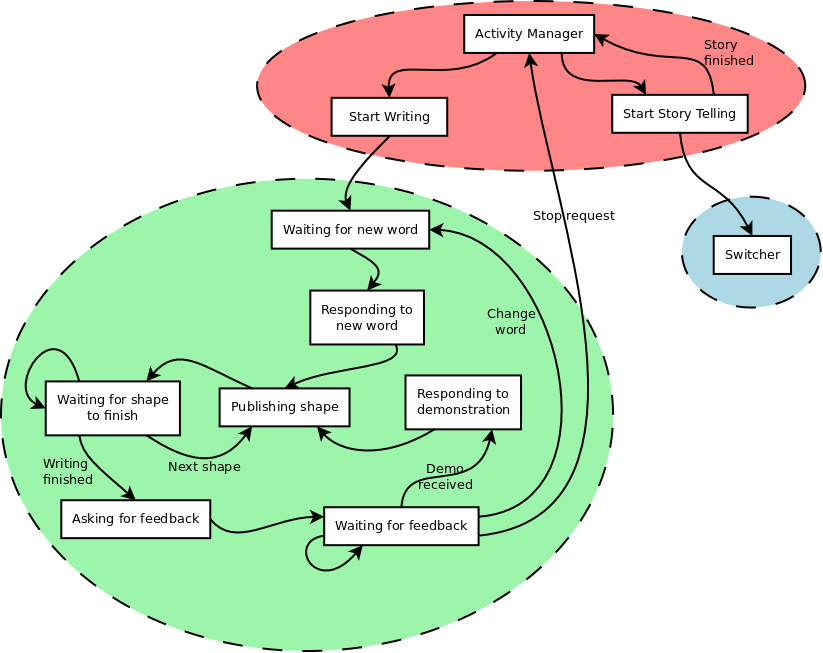
\includegraphics[width=0.75\textwidth]{figures/stateMachine.png}
        \caption{Framework implemented for in-situ studies}
        \label{fig:stateMachine}
\end{figure}

\subsection{Experimental design}

The experiment took place in Haut-Lac International School and 14 children in between 5 and 6 years took part of it. The children were organized in couples in order to find an emotional support with a known partner and allow a relaxed working environment.

\subsubsection{Scenario and procedure}
The experimental set-up (see figure \ref{fig:feasibility}) consists of the humanoid robot NAO, an external camera located between the feet of the robot and a tablet to interact with it. Additionally, during the experiment, two observers where located away from the interaction zone but having a face contact with the children interacting to assess engagement manually. Finally, the person guiding the activity or \textit{facilitator} was located at the left of the children. 

The two children in front of the robot interacting during 20 min each by turns. Each turn consisted on two activities; the original writing activity as an engaging one since intuitively is more interesting for children and a story telling as non-engaging, which was different for the two children. The main goal was to measure with the camera the features captured during both activities in order to find differences between them in terms of child attitude and behaviour.

\bigskip
\begin{figure}[h!]
        \centering
        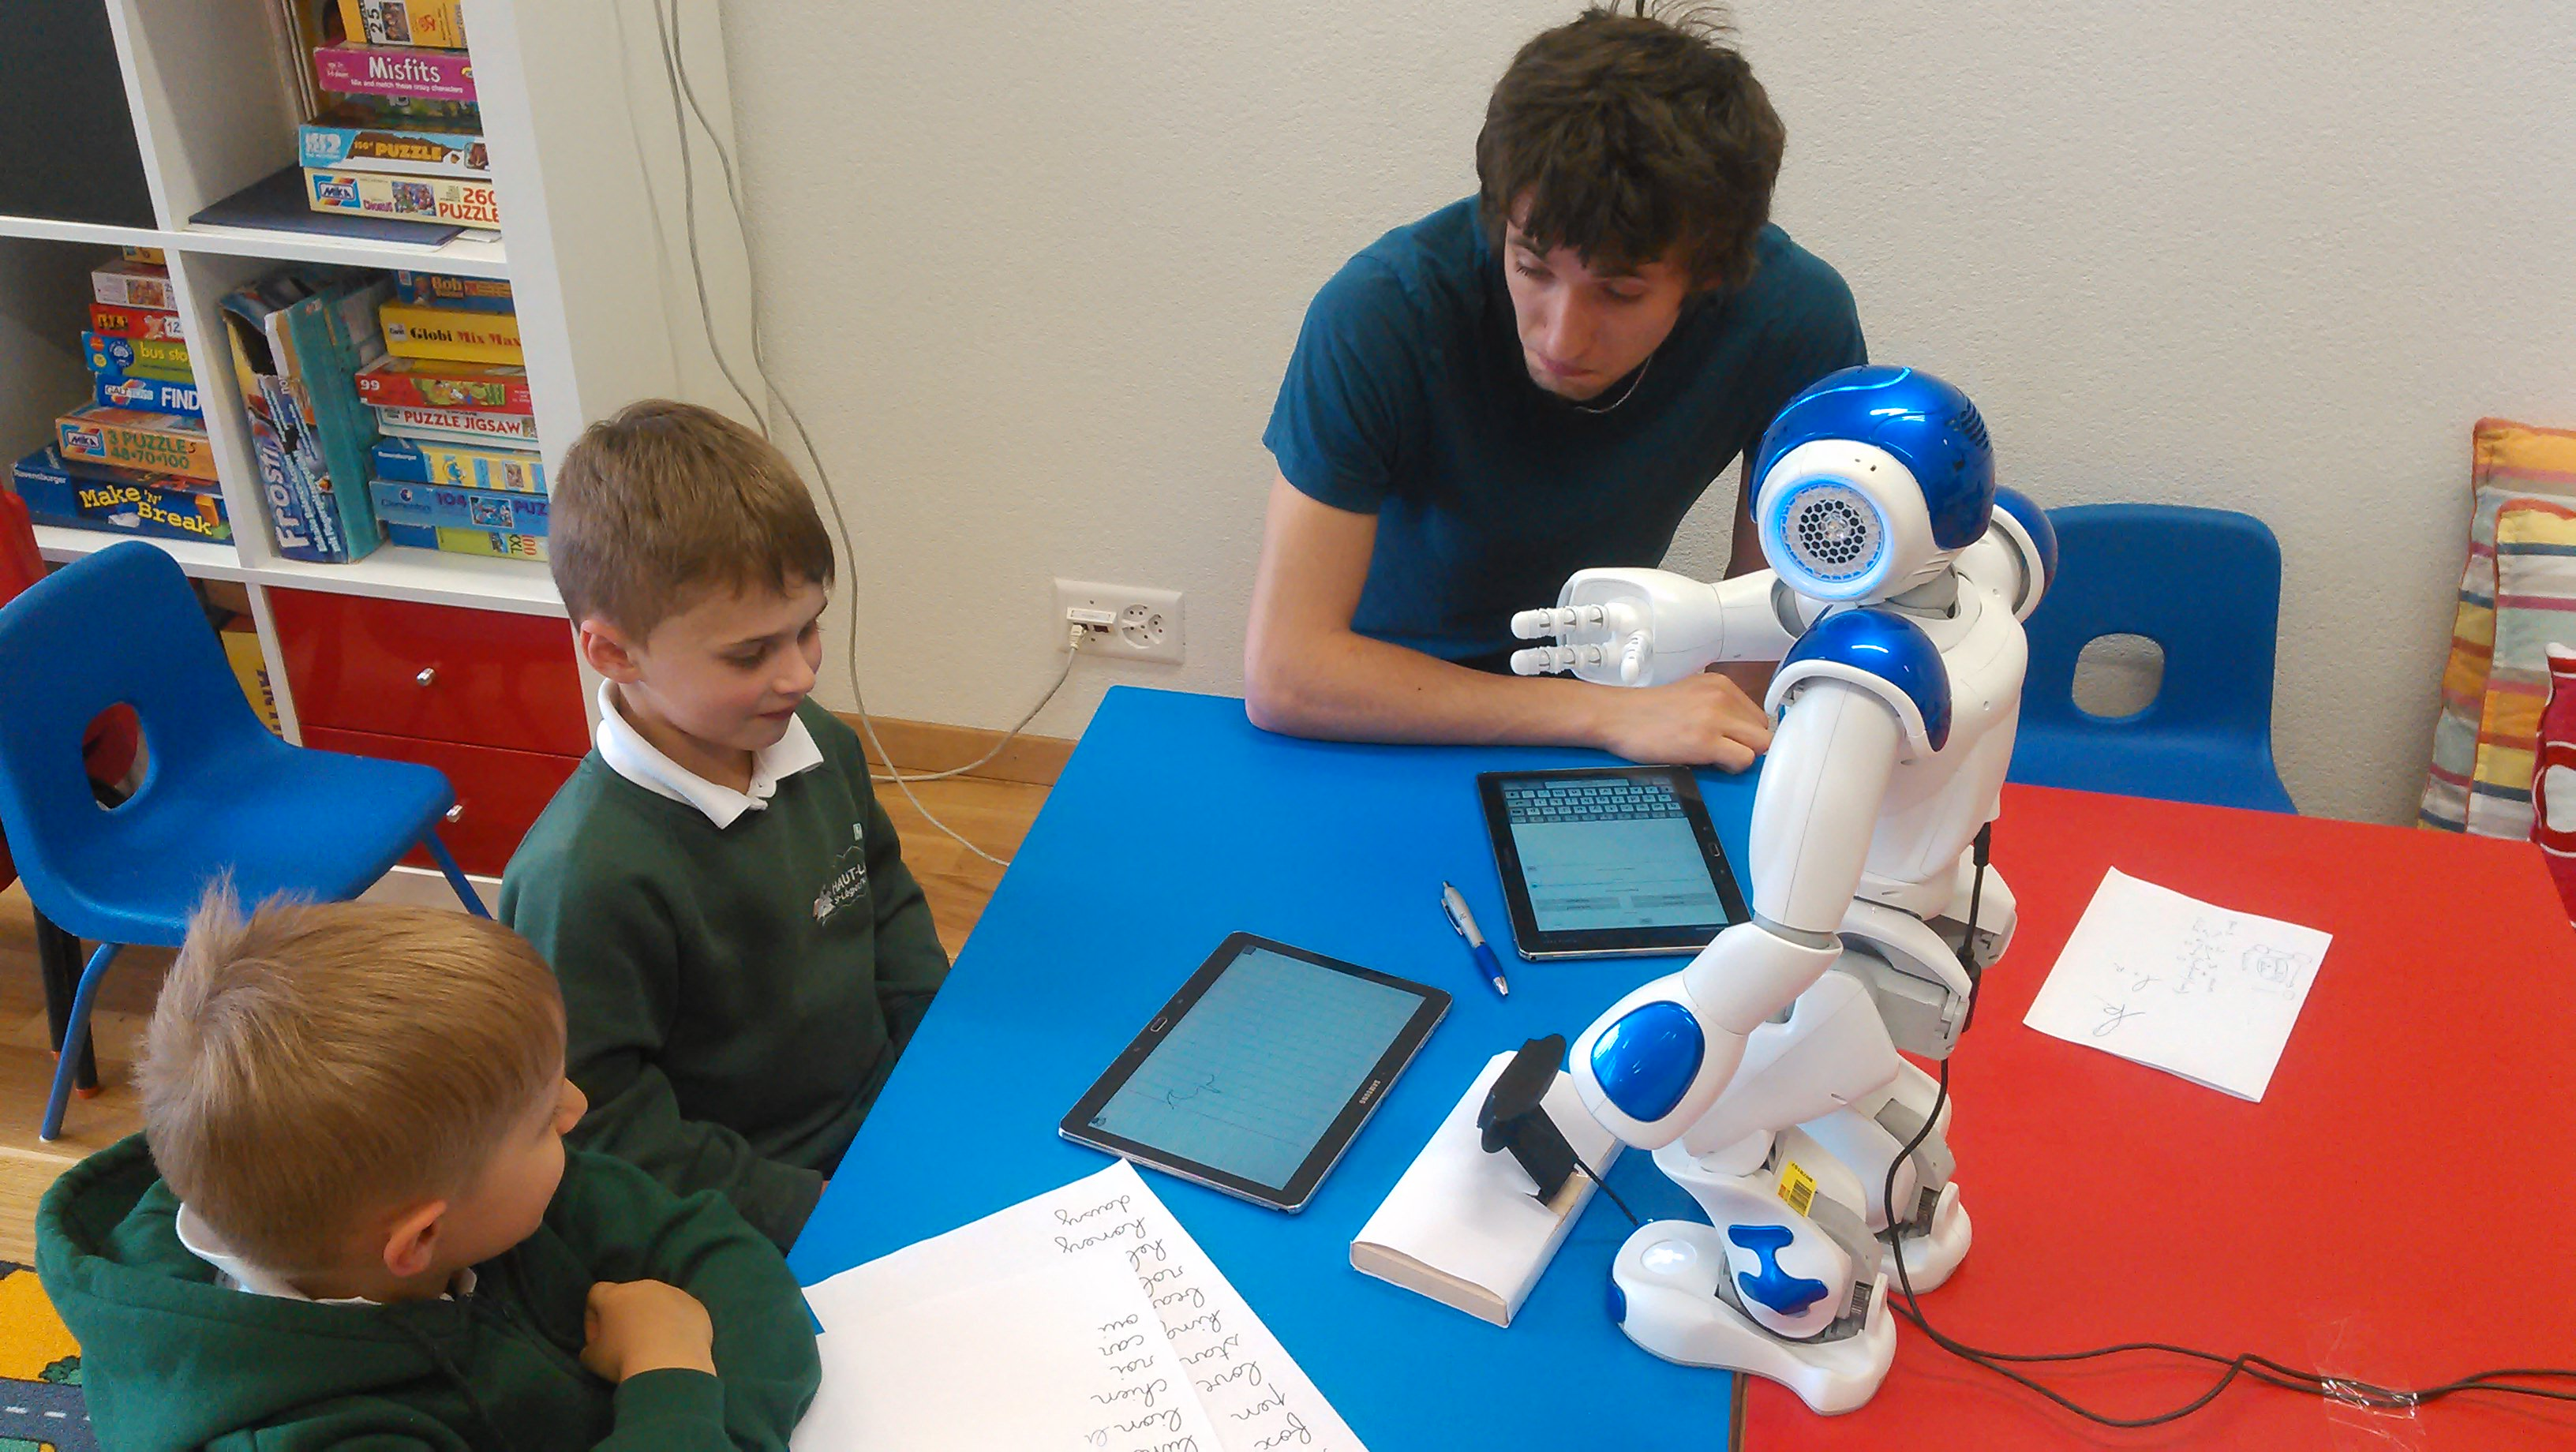
\includegraphics[width=0.7\textwidth]{figures/feasibility.jpg}
        \caption{Scenario during the feasibility test}
        \label{fig:feasibility}
\end{figure}

Therefore the goal was to obtain as much relevant data as possible in both, engaging and non engaging activities, to eventually be able to asses automatically when the child is one state or another.

\subsubsection{Measured variables} \label{measuredVariables}
During the activity the following variables were measured:

\begin{itemize}
\item Proximity to the region of interaction, robot and tablet.
\item Quantity of movement during both activities excluding the writing moments.
\item Gaze direction. Which side the child look to. 
\item Time response from the end of the robot demonstration till the stylus touch the tablet.
\item Time taken by the child to write the word.
\item Smile counter.

\end{itemize}
	

\subsubsection{Ground truth acquisition}
The ground truth is one of the most important parts of the data acquisition since it will be the reference point of the result analysis. As in many cases, it was necessary to acquire it during the experiment. In order to do that an Android ROS application (see figure \ref{fig:dataCollect}) was developed as a tool to help the assessment by the human observers.


\begin{figure}[h!]
        \centering
        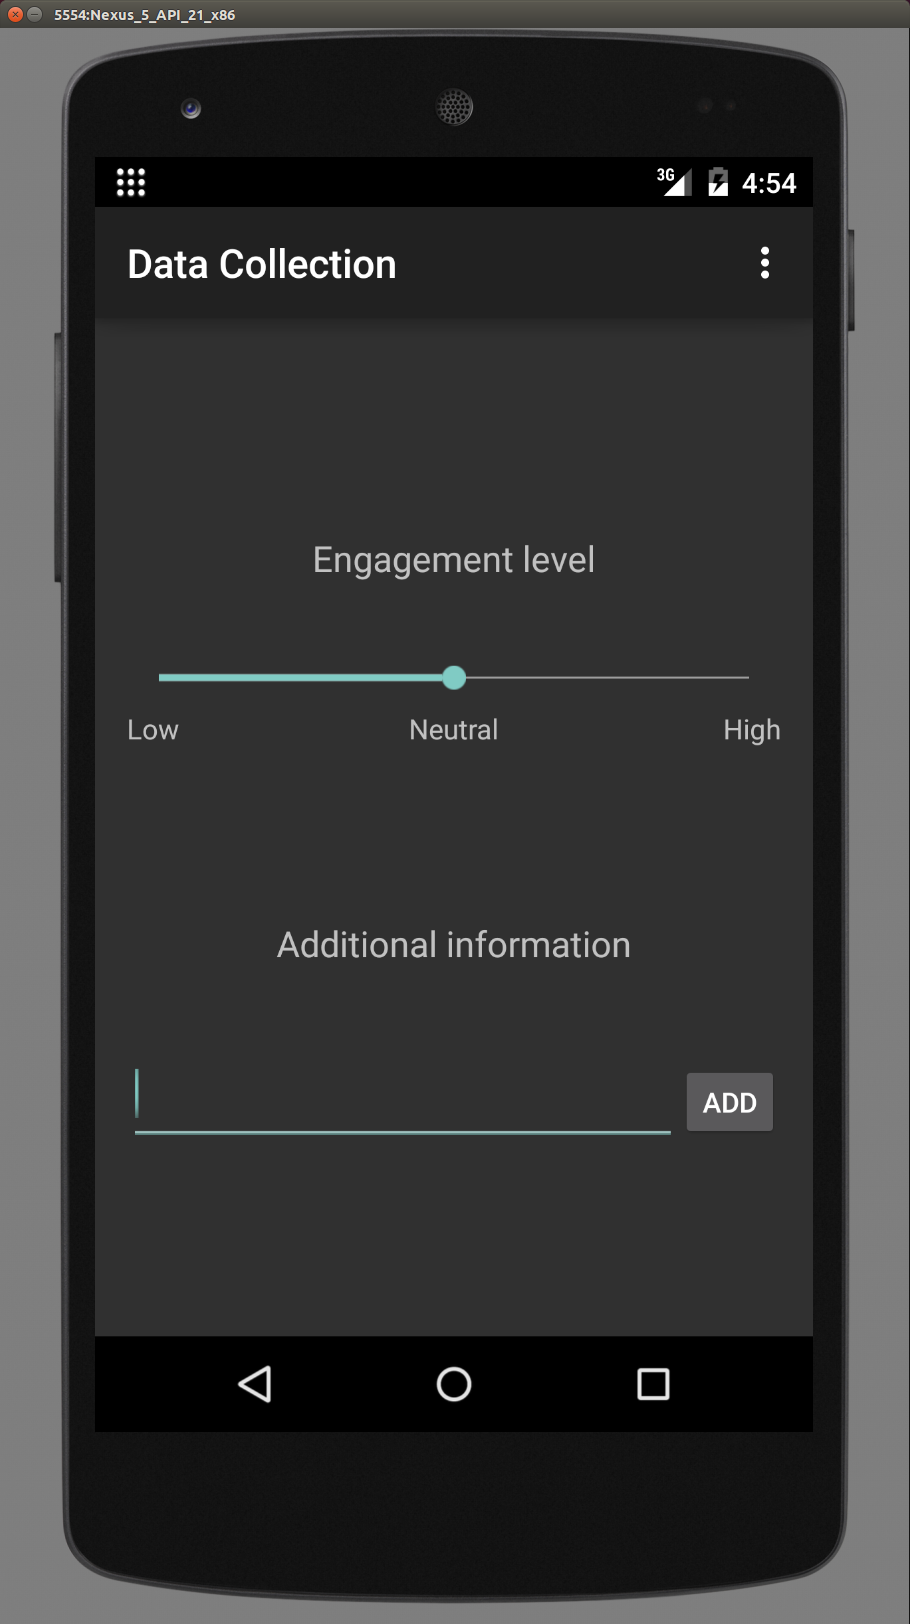
\includegraphics[width=0.3\textwidth]{figures/dataCollection.png}
        \caption{Engagement collection App for visual assessment}
        \label{fig:dataCollect}
\end{figure}


\subsection{Results}

We decided to provide a list of words to be chosen by the user in a sheet of paper. However, we quickly realized about the need of providing such words in a word selection application (see figure \ref{fig:wordSelector}) in order to smooth the interaction and the feeling of free choice. This simple Android ROS application publishes to the topic $ words\_to\_write $ when a button is pressed.

\begin{figure}[h!]
        \centering
        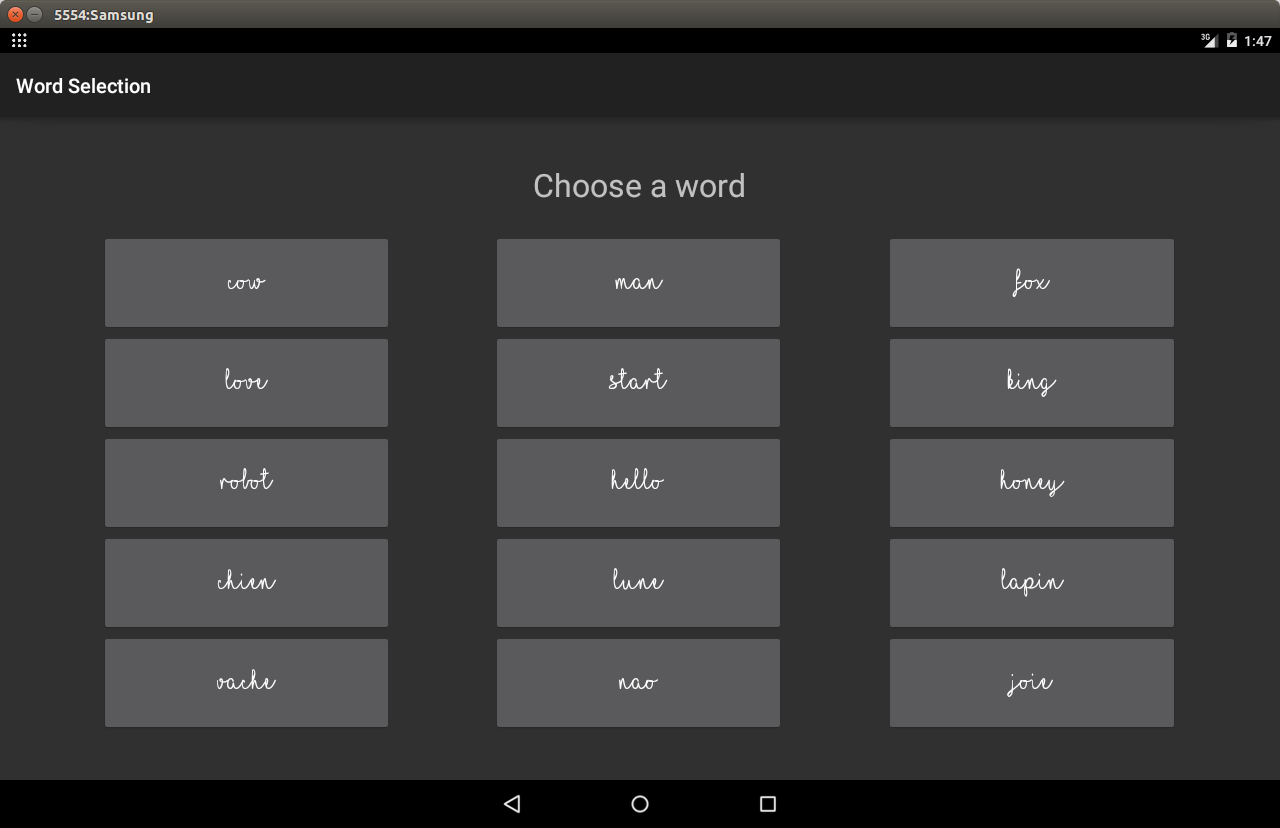
\includegraphics[width=0.7\textwidth]{figures/wordSelector.png}
        \caption{Word Selection App screenshot}
        \label{fig:wordSelector}
\end{figure}

Eventually, the data was acquired successfully and the application only crashed in two occasions during the 6 hours experiment. An experiment in a more controlled environment was scheduled and is presented in section \ref{sec:experiment}. However, several minor changes were reported and required to be fixed before that, such as:

\begin{itemize}
\item In order to correctly assess the level of engagement, it is necessary to minimize the human intervention. It turned to be a must that the experiment was for a single child. In addition, additional work was needed to better define the role of the facilitator and the human observers assessing the engagement.
\item The ground truth acquisition tool needed a simplification as well as a synchronization with the ROS master to be able to match the timestamps properly.
\item The age range was not the proper one in order to acquire writing samples and writing times to train the statistical engagement model proposed in Chapter \ref{chap:engagementModel}.
\item Several minor corrections related with the predefined speech of the robot and motion behaviour needed to be fixed.

\end{itemize}

\section{Data acquisition experiment} \label{sec:experiment} 
In this section the data acquisition through a formal experiment is explained in detail. However, the results extracted from this are discussed and analysed in detail in chapter \ref{chap:results}.
\subsection{Motivation}
After the feedback acquired in the first intervention through the feasibility study and the changes applied, it was necessary to go back to the field to collect data such as: shape letters, time and writing responses, gaze directions, quantity of movement and proximity distances, with a more stable system and improved protocol.


\subsection{Expected outcomes}

The desired outcome is the collection of all relevant information cited in section \ref{measuredVariables}, possibly related with the level of engagement, in order to tune the system to be able to give suggestions allowing long-term use with children. However, it also includes

\begin{itemize}
\item autonomous adaptive behaviours based on real-time information,
\item the data acquisition to detect correlations between the features tracked and the level of engagement and,
\item the acquisition of a ground truth model using the visual assessment of two observers during the interaction.

\end{itemize}

\subsection{Experimental design}
In this case, the experiments were scheduled in the International School of Geneva on June 5th, 2015 and 6 participants were involved.

\subsubsection{Scenario and procedure}
The experimental set-up (see figure \ref{fig:experiment}) consists of the humanoid robot NAO, an external camera located in the base of the robot and two tablets to interact with the robot: One where the CoWriter displays and collects the user demonstrations, and another one to select the word to write. In similar manner as in the feasibility study, the two observers where located away from the interaction zone but having a face contact with the children interacting. Finally, the person guiding the activity or \textit{facilitator} was located at the left of the children. 

\begin{figure}[h!]
        \centering
        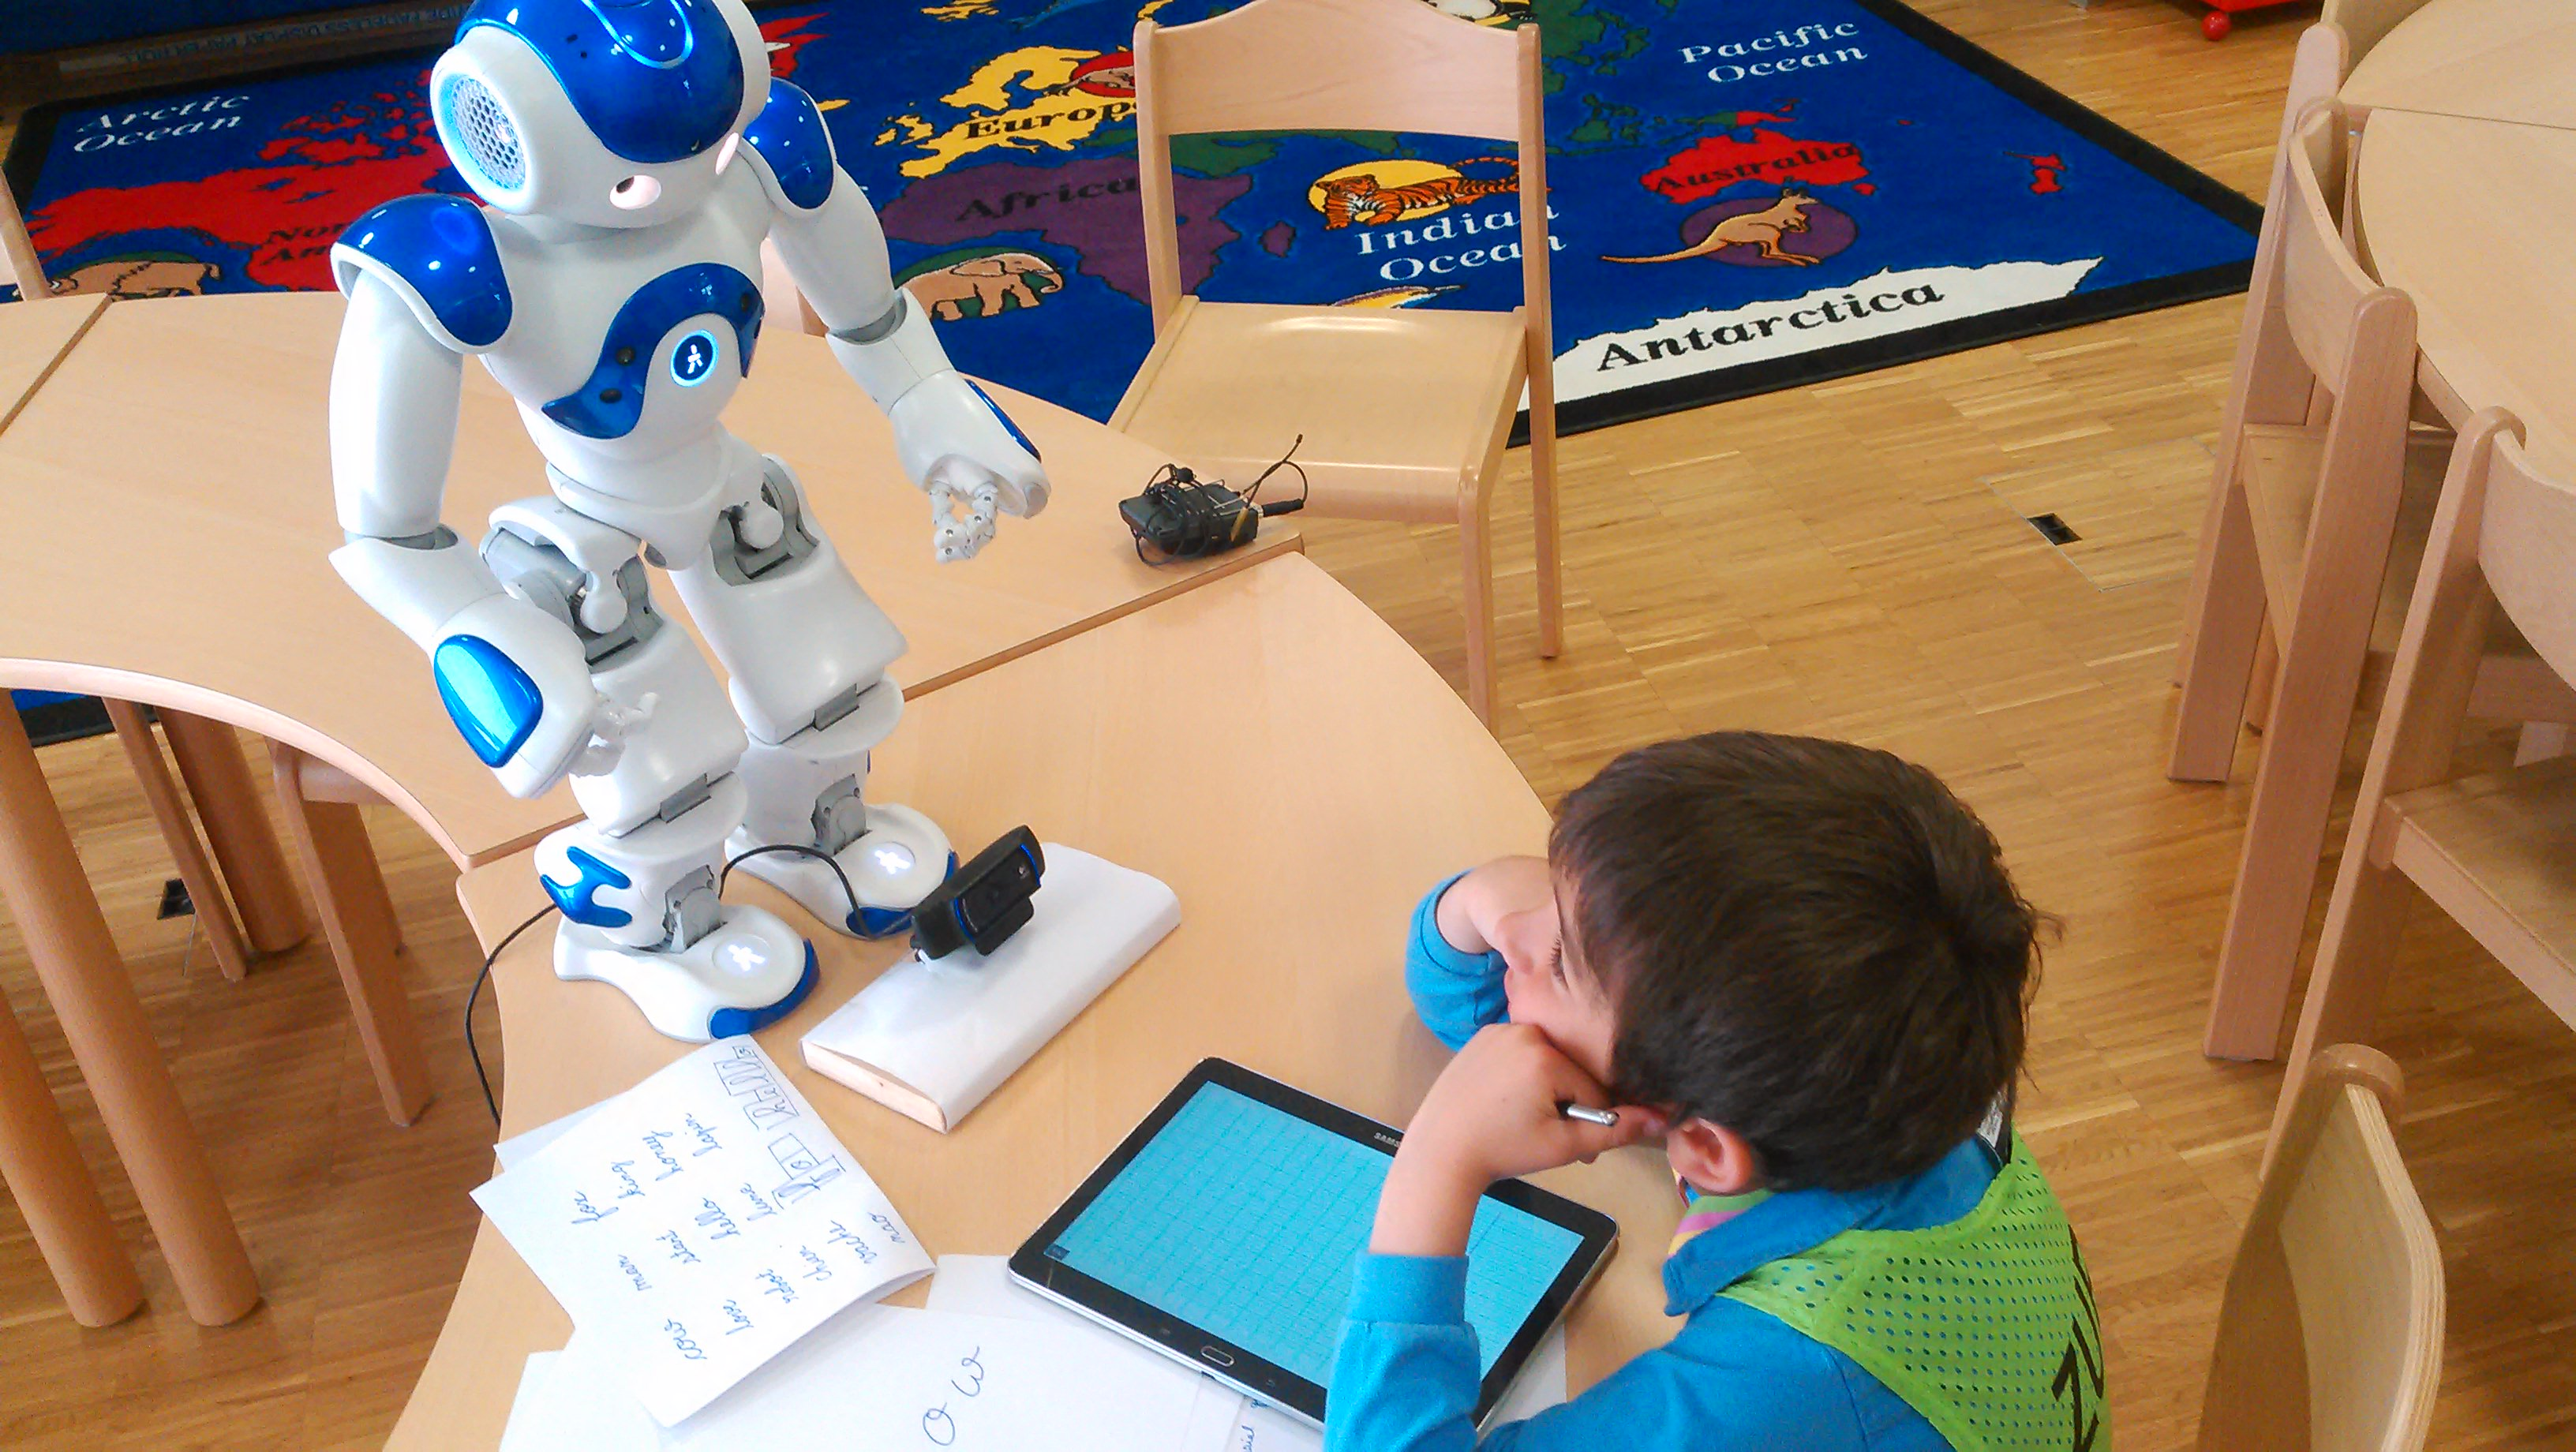
\includegraphics[width=0.7\textwidth]{figures/experiment.jpg}
        \caption{Redefined scenario during the experiments.}
        \label{fig:experiment}
\end{figure}

In this case, only one child interacted with the robot for 20 min. During this time, two activities were run; the original CoWriter (writing activity) as engaging task and the story telling as non-engaging. During this time the variables measured were the same as in section \ref{measuredVariables}.


\input{experiment.tex}
\chapter{Analysis of the Results and Discussion} \label{chap:results}

\section{Measurement of engagement ground truth}
The acquisition of the grand truth was performed by two different observers that were not into the interaction field, but with direct vision towards the subjects. A result of that visual assessment is shown in figure \ref{fig:GTexample}. The rest of the results are shown in the appendix \ref{appendix}.

\begin{figure}[h!]
        \centering
        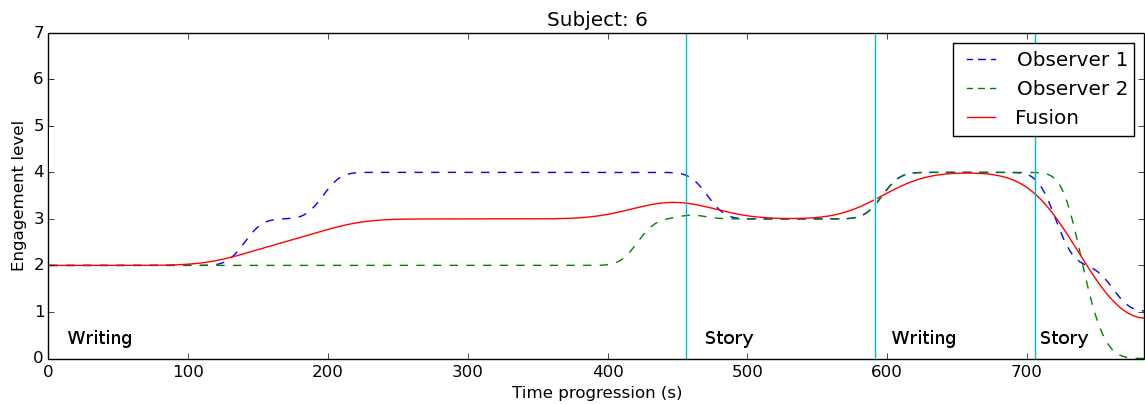
\includegraphics[width=0.6\textwidth]{figures/GTexample.png}
        \caption{Example of grand truth acquisition and fusion. The vertical lines indicate the story telling activity.}
        \label{fig:GTexample}
\end{figure}

It is important before comparing any result to check the inter rater reliability of the two observers, in another words, the inter-rater reliability for the ground truth. This measurement shows if the data can be used, or not, for that specific purpose of comparison and reference with respect to the feature measurements acquired. 

In order to do that, it is necessary to apply an arithmetic mean to the engagement value assessed by each of the observers taking into account each child in both CoWriter (writing) and story telling activities. Then, applying a Cronbach's alpha test (see equation \ref{eq:cronbach} in appendix), In this case, $\alpha = .82$ over the 6 subjects showing an agreement between both observers.

Furthermore, a one-way between groups ANOVA was run to see any relevance between the assessment measurement in both activities. In another words, if the measurements show enough variance to be used as ground truth. The result obtained was: $F[1,22] = 9.07 \quad p=.006$ (see appendix \ref{ap:GT}), which reveals that the activities lead to significantly different level of engagement.


\section{Movement and proximity across the two activities}
For quantity of movement (QoM) and proximity respectively, in both cases, greater means correspond to the writing activity as we can see in figures \ref{fig:meanMov} and \ref{fig:meanProx}. It leads to the assertion that the QoM and the proximity are directly related at least, with an active or passive activity.

Since the population studied does not exceed the 6 participants, we can not assume the data is normally distributed thus a T-test makes an estimation of the deviation instead of the real value considering a peer-wise comparison.

The results obtained from the T-test for both features shows a marginal significance in the QoM $ (t(df=10)= 2.0964, p = 0.06245) $ and significance \footnote{There is significance when $p<0.05$ and marginal significance when $p<0.1$} for the proximity measurement $(t(df=9.7406)= -2.8338, p = 0.01818) $. In addition, mean and standard deviation are shown in table \ref{tab:pvalues}.

\begin{figure}[h!]
        \centering
        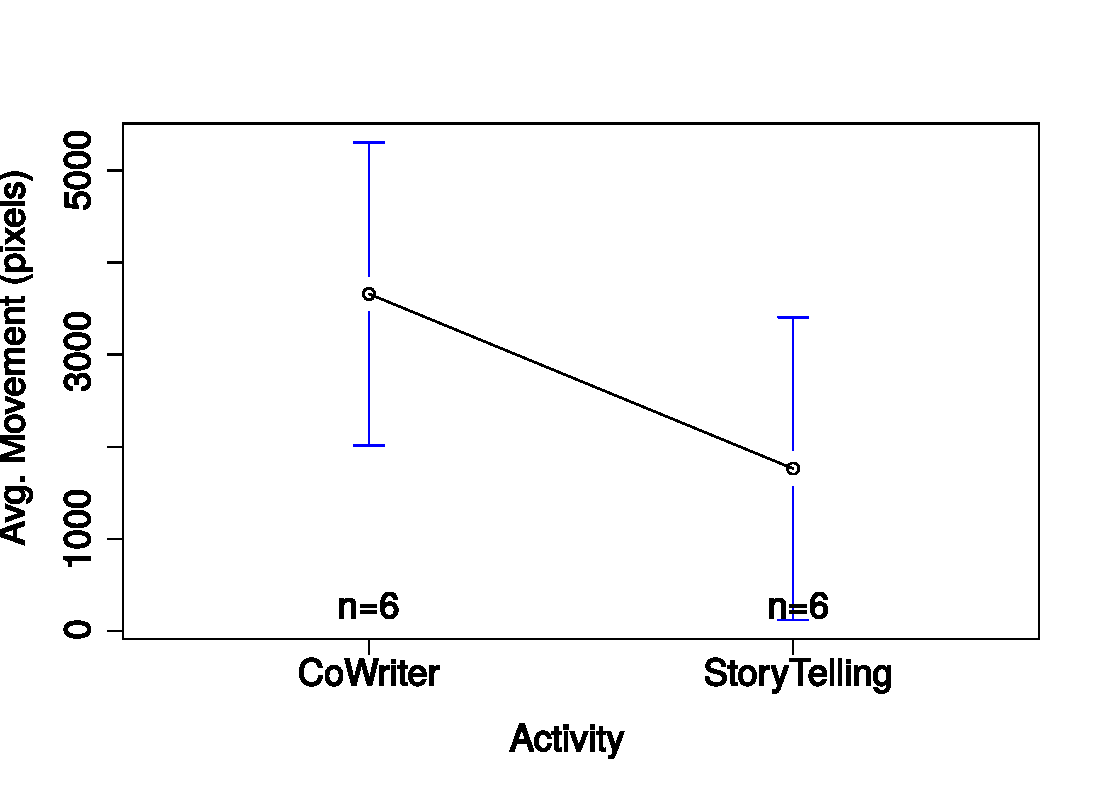
\includegraphics[width=0.7\textwidth]{figures/AvgMovement}
        \caption{QoM mean plot(ends show the confidence interval) across the two activities.}
		\label{fig:meanMov}
\end{figure}


\begin{figure}[h!]
        \centering
        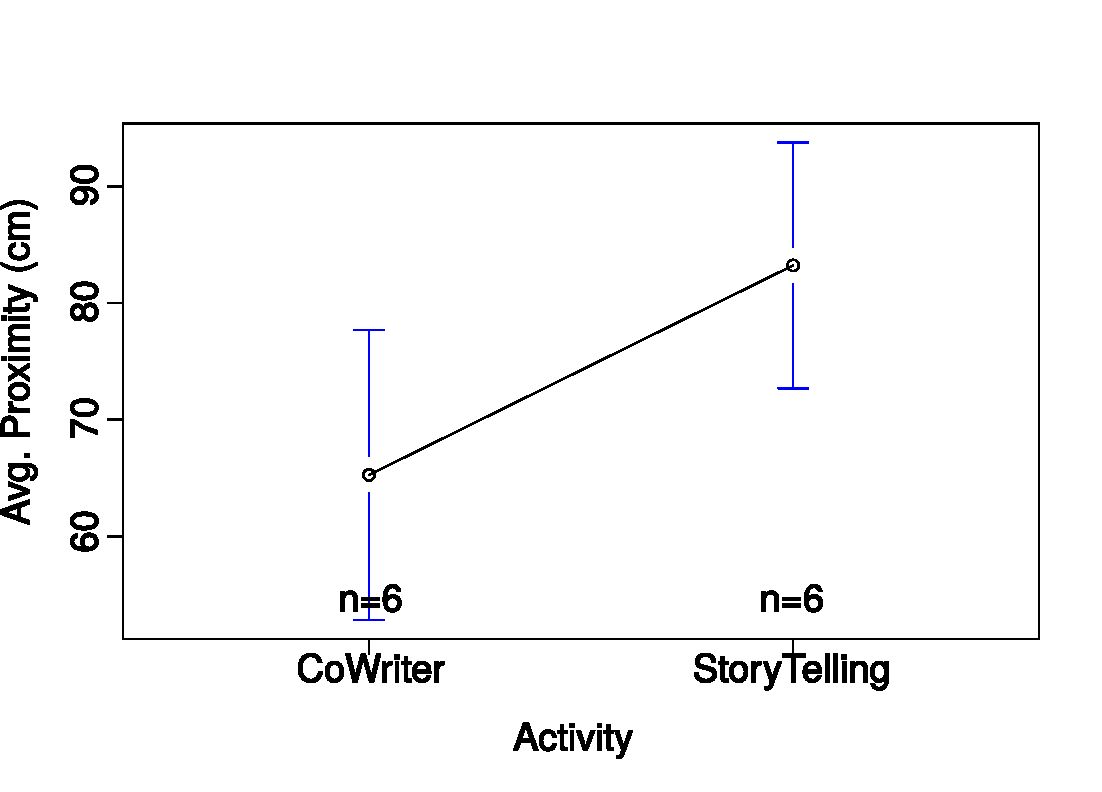
\includegraphics[width=0.7\textwidth]{figures/AvgProximity.pdf}
        \caption{Proximity mean plot(ends show the confidence interval) across the two activities.}
		\label{fig:meanProx}
\end{figure}


\begin{table}[h!]
\centering
\begin{tabular}{l|l|l|l|l}
          & \multicolumn{2}{c|}{\textbf{Writing}}                               & \multicolumn{2}{c|}{\textbf{Story telling}}                        \\ \cline{2-5} 
          & \multicolumn{1}{c|}{$\mu$} & \multicolumn{1}{c|}{$\sigma$} & \multicolumn{1}{c|}{$\mu$} & \multicolumn{1}{c}{$\sigma$} \\ \hline
\textbf{QoM}  &          3658.783                  &         1567.510                      &              1763.050              &              1564.938                \\ \hline
\textbf{Proximity} &      65.26000                      &           11.83703                    &          83.21667                  &              10.04000                
\end{tabular}
\caption{T-test mean, $\mu$ and standard deviation, $\sigma$ (see appendix \ref{ap:across}).}
\label{tab:pvalues}
\end{table}


However, a more accurate measurement across groups is performed by an ANOVA. In this case, a one way repeated measures ANOVA was used since we have a single group (6 subjects) on which we have measured the QoM and the proximity a few times (for writing and story telling activities) during the same amount of time. The results shown a significance \textit{F[1,115]=21.01, p=1.17e-05} being \textit{p<.001} for proximity and no significance for QoM \textit{F[1,286]=0.729, p=0.394}.

As we can see, the proximity measurement is significant. Therefore, the proximity to the interaction field is a good indicator of the child engagement in an active activity. In addition, the results are consistent with the lines shown in figures \ref{fig:anovaMov} and \ref{fig:anovaProx}, where in both cases the two groups are rather close together. However, relevant information can be extracted from the test output. The within subject test indicates that there is a significant relation between subjects, in other words, the groups do change between subjects but preserve a similar difference between activities. It shows that not all subjects share the same rank of movement and position.

\begin{figure}[h!]
        \centering
        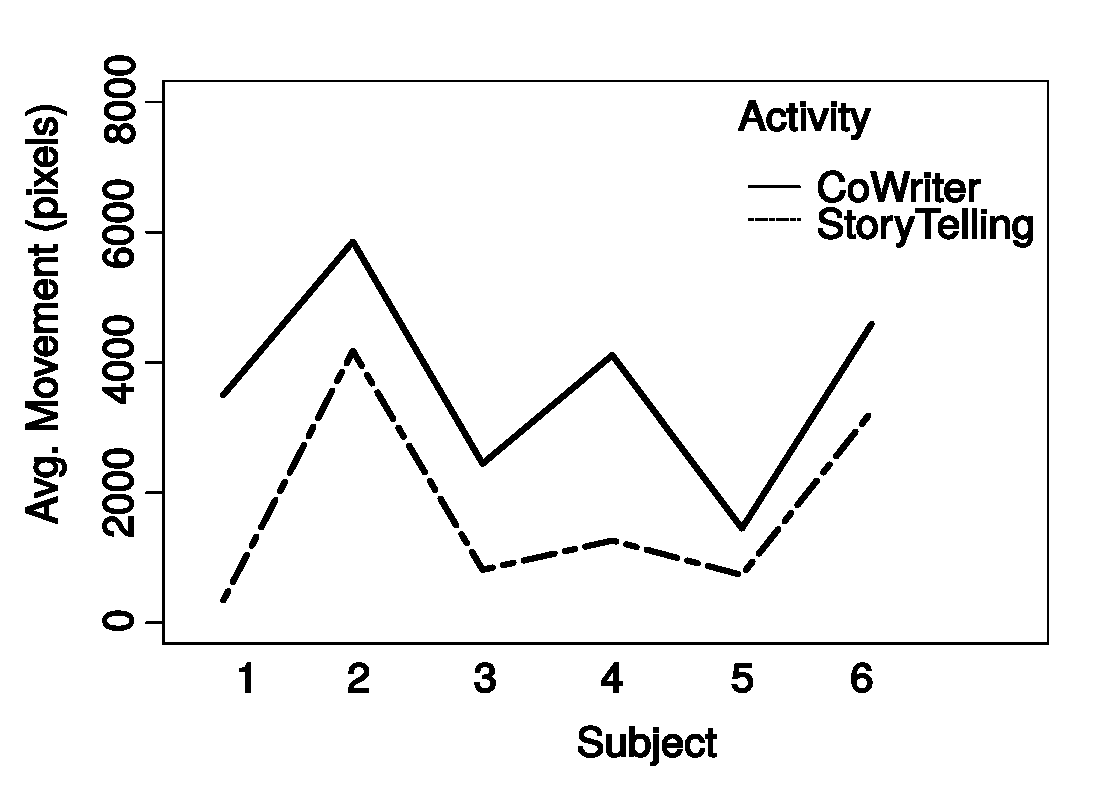
\includegraphics[width=0.7\textwidth]{figures/AvgMovement2.pdf}
        \caption{Inter-subject measurement variability for QoM.}
		\label{fig:anovaMov}
\end{figure}

\begin{figure}[h!]
        \centering
        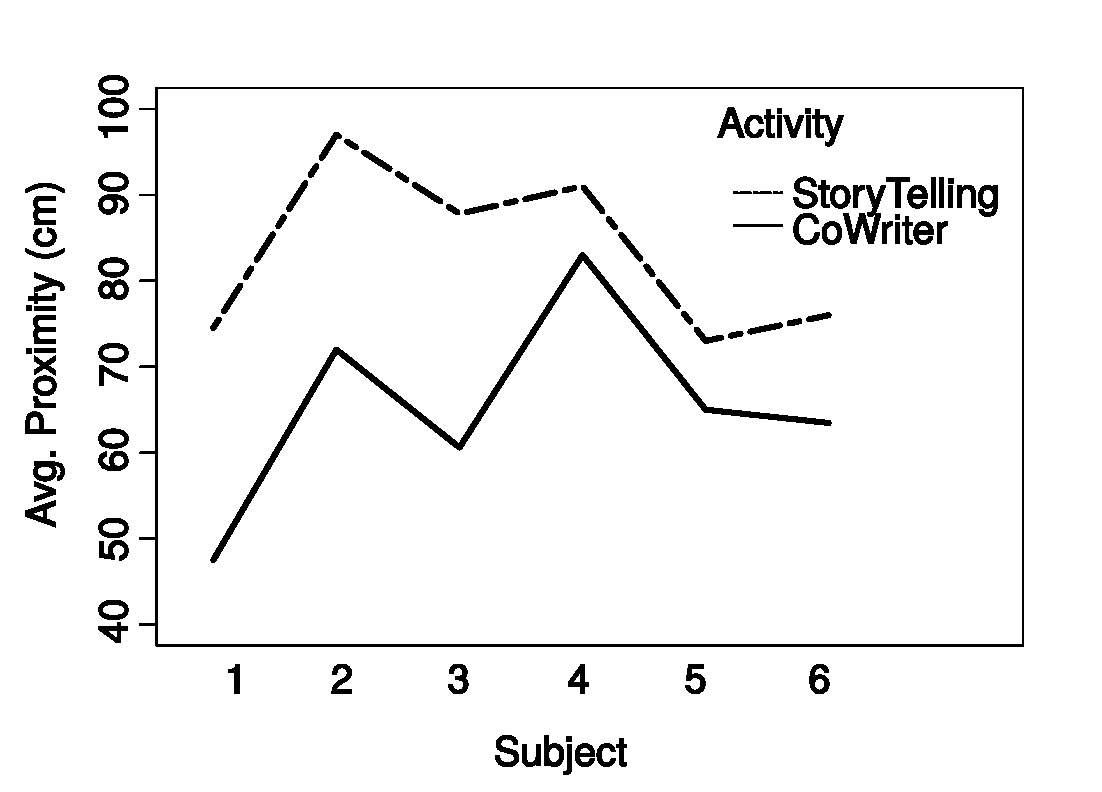
\includegraphics[width=0.7\textwidth]{figures/AvgProximity2.pdf}
        \caption{Inter-subject measurement variability for proximity.}
		\label{fig:anovaProx}
\end{figure}

It is necessary to say that these results need to be contrasted evaluating a greater number of subjects.
\\\\\\
Finally, in figure \ref{fig:avgProximity} we can see the average normalized proximity between the subjects over time, where the vertical lines indicate the story telling starting point in each case. In 5 over 6 subjects there is a tendency to decrease the proximity to the field of interaction right after the execution of the story telling activity.

\begin{figure}[h!]
        \centering
        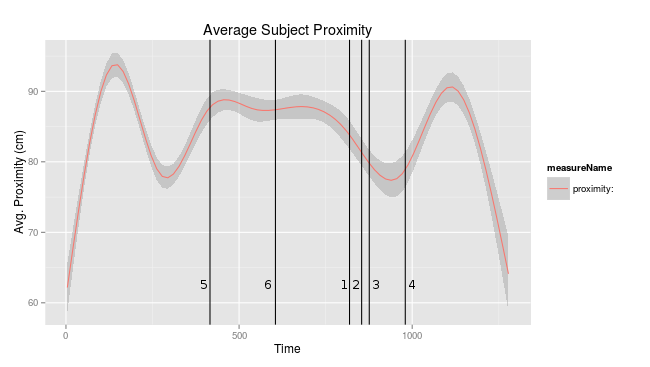
\includegraphics[width=1\textwidth]{figures/avgProximity.png}
        \caption{Average proximity measurement between subjects. The vertical lines indicate the start of the story telling activity.}
        \label{fig:avgProximity}
\end{figure}

\section{The gaze information}

After a preliminary analysis of the gaze direction, we noticed that in this specific context this feature does not provide a reliable measurement of engagement. However, it becomes interesting from the interaction point of view, being able to show the amount of intervention \ref{fig:gaze} needed from the facilitator sitting on the left of the subject, against the visual contact towards the field of interaction (robot and tablet).


 \begin{figure}[!htb]
	\centering
	\begin{tikzpicture}[>=latex]

		\node[inner sep=0pt] (xtion) at (0,0) {
		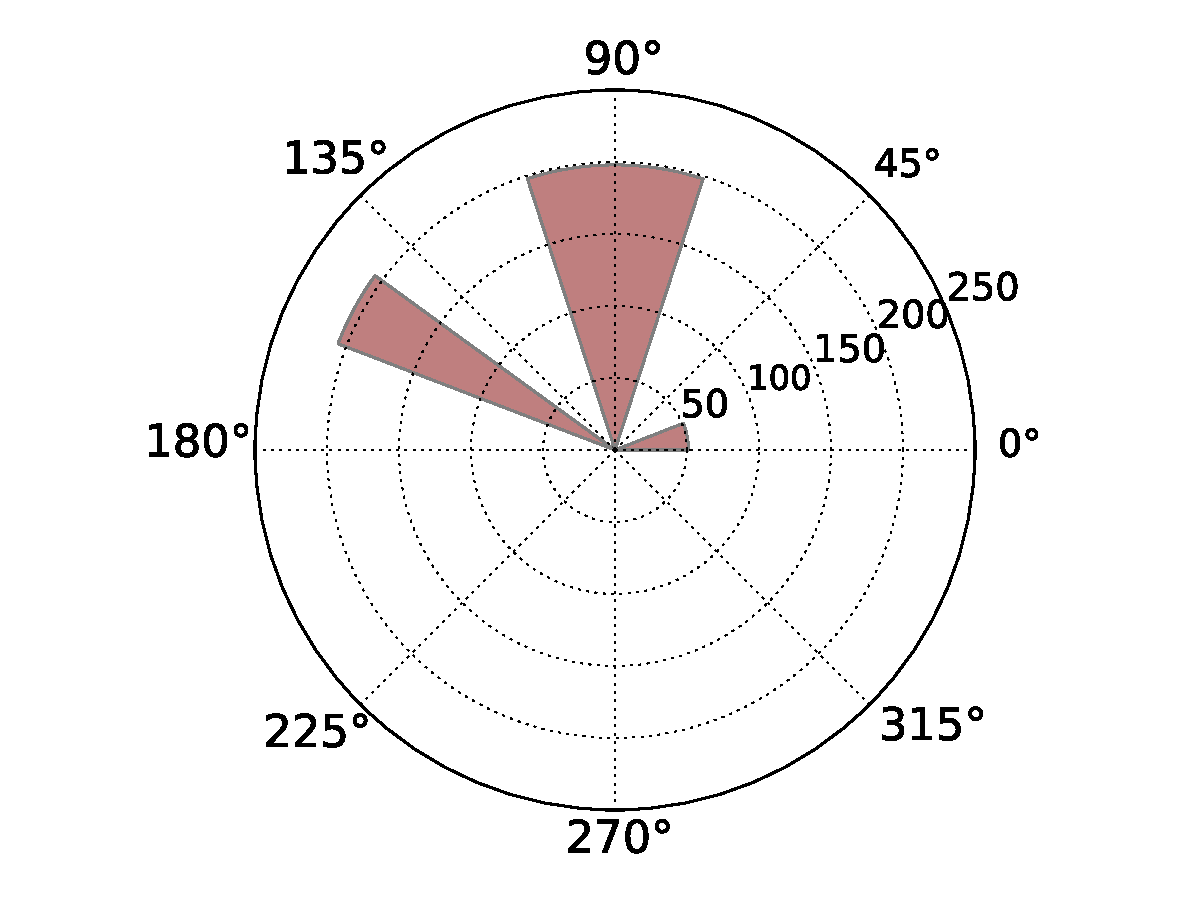
\includegraphics[width=0.6\textwidth]{figures/gaze.pdf}};
	
		\node[black, text width=2cm] at (0.74,1.8) {		
		Robot	
		};
		
		\node[black, text width=2cm] at (-1.3,0.5) {		
		Facilitator	
		};
				
	\end{tikzpicture}
    \caption{Subject's mean gaze direction being the $ 90\degree $ the robot and tablet together, and the range comprised between $ 135\degree-180\degree $ the location of the facilitator.}
    \label{fig:gaze}
\end{figure}

Using a range of age comprised in between 5-6 years old requires a high level of intervention. In this study, this accounts for almost half percent of the interaction time spend in front of the agent. Therefore, we can hypothesize that during the writing activity the children look more to the left and less to the robot in comparison with the story telling activity.

It is also important to test how likely it is that an observed distribution is due to chance or not using Pearson's Chi-squared (see equation \ref{eq:chi} in appendix). The result $(\chi^2(df=6,  N=537.75), p-value < 2.2e-16)$ shows a tiny chance. Secondly, in order to verify the hypothesis formulated previously based on one subject observation, we can use the residuals of the Chi-squared test comparing the observed data. The results are summarized in table \ref{tab:chi}.

\begin{table}[h!]
\centering
\begin{tabular}{l|l|l|l|l}
 		 		  & \textbf{Down} & \textbf{Left}	& \textbf{Right} & \textbf{Robot}	    \\ \hline	
 \textbf{Writing} &  102(3.4811216) & 2965(4.454916) & 35(-0.1499802)  &  993(-7.701501)    \\ \hline
 \textbf{Story telling}    &    0(-1.1542352) & 215(-10.687569)      & 6(0.3598100)      & 371(18.476290)
\end{tabular}
\caption{Chi-square test results (see appendix \ref{ap:across}).}
\end{table}\label{tab:chi}

As we hypothesize, the users tend to change their gaze direction towards the \textit{facilitator} located to left and to the tablet during the writing activity whereas the attention towards is acquired during the story telling activity. It suggests a future improvement towards a more independent system in the writing activity.


\chapter{Conclusions} \label{chap:conclusions}

It has been a long process from the design till the testing phase. Due to the variety of technologies used as well as the number of experiments scheduled, several conclusions can be extracted from both the mathematical and the socio-educational point of view. The challenges involved in developing such a technology which have been addressed in this work include:

\begin{itemize}
\item Real-time robot adaptive behaviour based on face features.
\item Robust face detection acquisition.
\item Engagement assessment using visual and non-visual measurements.
\item Improvement of the user experience by addition of new features.
\item Correctness assessment of shape's letters. 
\end{itemize}

Based on Chapter \ref{chap:correctness}, we have provided a good metric based on SVM for handwriting shape classification but also City block distance for shape comparison in the eigenspace. In addition, the output clustered provided allow us to classify and check the most common errors in children letter writing if we need it. Moreover, part of this outcomes has been used  and embedded in an Android-ROS application with the goal of providing the assessment information to the facilitator. 

The adaptive behaviour model propose based on online acquisition of user information such as proximity, quantity of movement and gaze direction among others, seems to be a good way to model a rich set of behaviours according to the specific context of the situation. In addition, it allow us to smooth the interaction during the activity with the child without colliding in the use of the same robot resources and acting independently of the activity performed.  

One of the most important outcomes of Chapter \ref{chap:feasibility} on the technical aspect has been the extension of the current state machine framework, allowing the addition and transition among different activities. Therefore, the new framework allows the definition of new activities and the condition of transition between them in a flexible and easy way. Furthermore, the feasibility study shows how deterministic can be the choice of the age range in an educational context as well as the protocol of the experiment in to reduce external factors that could influence in the data acquisition. For instance, part of the movement captured during the activity could have been induced by external factors such as the facilitator providing explanations, so it is a must although not trivial to anticipate this measurement for its subtraction.

Due to the previous assumption, the gaze of the children by itself can not be a reliable indicator for child's engagement neither, at least based on the current implementation (a better suggestion would be the use of an eye tracker). However, it has been very useful in the quantification of the facilitator involvement in the activity. It proves that the percentage of implication of the person helping during the activity time, specially in the CoWriter, is high. Therefore, it would be necessary to continue working on the automation of the system reducing the human intervention using better explanation or self-descriptive interactive situations.

Finally, the use of the child's face proximity to the field of interaction as an indicator of engagement in the specific context of the writing and the story telling activities it is significant since in most of the cases the proximity decreases during a non-engaging and passive task.

\section{Future work}

Additional work needs to be done in two aspects in particular: The robot independence from the facilitator and the online engagement detection for practical use.  

The independence of the system without requiring any human intervention is the most complex and challenging one. It is necessary to design interaction protocols with a continuous and quick feedback to the user. For instance, the system has been improved from the interactivity and flexibility points of view, adding an Android application that publishes the desired word written by the facilitator, or the one corresponding to the button pressed by the child. However, it slightly adapts to short-term events such as a gesture generation according to the context of activity. For instance, a good performance in the writing of a word, should lead to show a positive gesture from the robot that would reinforce the children interacting.

To solve the previous limitation it would be necessary to expand the current model to be able to provide two outputs: Behaviours and gestures, long-term and short-term responses respectively. A reasonable approach would be to design two different internal ways of motion externalization. But also the improvements of certain functionalities such as the detection of the engagement level need additional work. Actually, it needs to be properly tested by the acquisition of the suitable children data; the writing responses and the correct assessment of the shape quality from 7 years old children with handwriting problems but with previous knowledge.

Apart from the two previous points, several minor changes and long term non-trivial implementations could be done. An example, is an improvement of the current version of the $ nao_writing $ package, responsible for the hand movements during the writing process, to perform them smoother and more accurate. Moreover, the aspect to consider in the long term would be to be able to execute the whole Cowriter system without a computer. Thus, it would be useful the optimization of the code to run in the internal NAO processor (Intel Atom 1.6 GHz). In this way, it would allow an easy set-up that could be easily prepared by a non-technical user.

Currently, the system has been tested in a real context with a 6 years old child with several difficulties in the acquisition of the handwriting supervised by a ergo-therapist in Geneva. The feedback extracted so far has been extremely valuable to redefine the current procedure as well as to point the most necessary improvements for a real scenario. But the most relevant outcome will be to test the system efficiency in the child handwriting improvement during a long term intervention.

Finally, in order to maximize the use of the landmarkers provided by dlib and at the same time allow the agent to know, not only about the child but also about the environment, would be possible to extract the 3D head pose estimation. Moreover, using a predefined 3D map with the most relevant things or people in the room, it would be possible to make the robot aware of the focus of attention of the child in the room at any moment.

On the educational side, open questions include how the handwriting error generation of the
system may be abstracted to a higher level of control so that a teacher may configure it to work
with a child on a particular type of mistakes, based on the child’s performance. Where would
the balance lie between developing autonomous capabilities for the system to determine the
child’s difficulties, and empowering the teaching staff to decide for themselves instead? And,
as a result, the most important question in this area is to address what impact to the outcomes of a handwriting intervention the addition of such a teachable robotic agent would have.

\appendix
\chapter{Student-Oriented Outcomes} \label{appendix2}

In addition to the theory presented in the previous chapters, a wide range of hands-on technical
content was required to be mastered in order to develop the research presented in this work.
Aspects which the author had limited or null experience with beforehand include:

\begin{itemize}
\item Development of Android applications.
\item ROS development (rosjava, installation from source, make files, etc.).
\item Use of Java, Python and C++ (over 700, 1500 and 800 lines written, respectively).
\item Use of \textit{dlib} library.
\item Development under Linux.
\item Use of github for version control, code re-view and collaboration.
\item Configuring of networks between devices.
\end{itemize}

Having undertaken the work in a research lab, there are also numerous practical non-technical skills which are transferable to future projects that have been built upon, including

\begin{itemize}
\item Demonstrations to laboratory visitors and others:

- Anara Sandygulova from University College Dublin on 14th April.

- Wafa Johal from Universit\'e de Grenoble on 5th May.

- Pooyan Fazli from Carnegie Mellon University on 16th April.

- Representatives of HKSTP, an R\&D company.

\item Conduction of user studies to adjust the direction of prototypes under development.
\item Presenting research to non-technical audiences such as:
		- Ergo therapist in Lausanne.
		- Ergo therapist in Geneva.
\item EPFL Open days.
\item CoWriter project meeting in IST Lisbon (Portugal).

\end{itemize}

\chapter{Additional results} \label{appendix}

\section{Ground truth engagement measurement} \label{ap:GT}

\begin{figure}[h!]
    \centering
    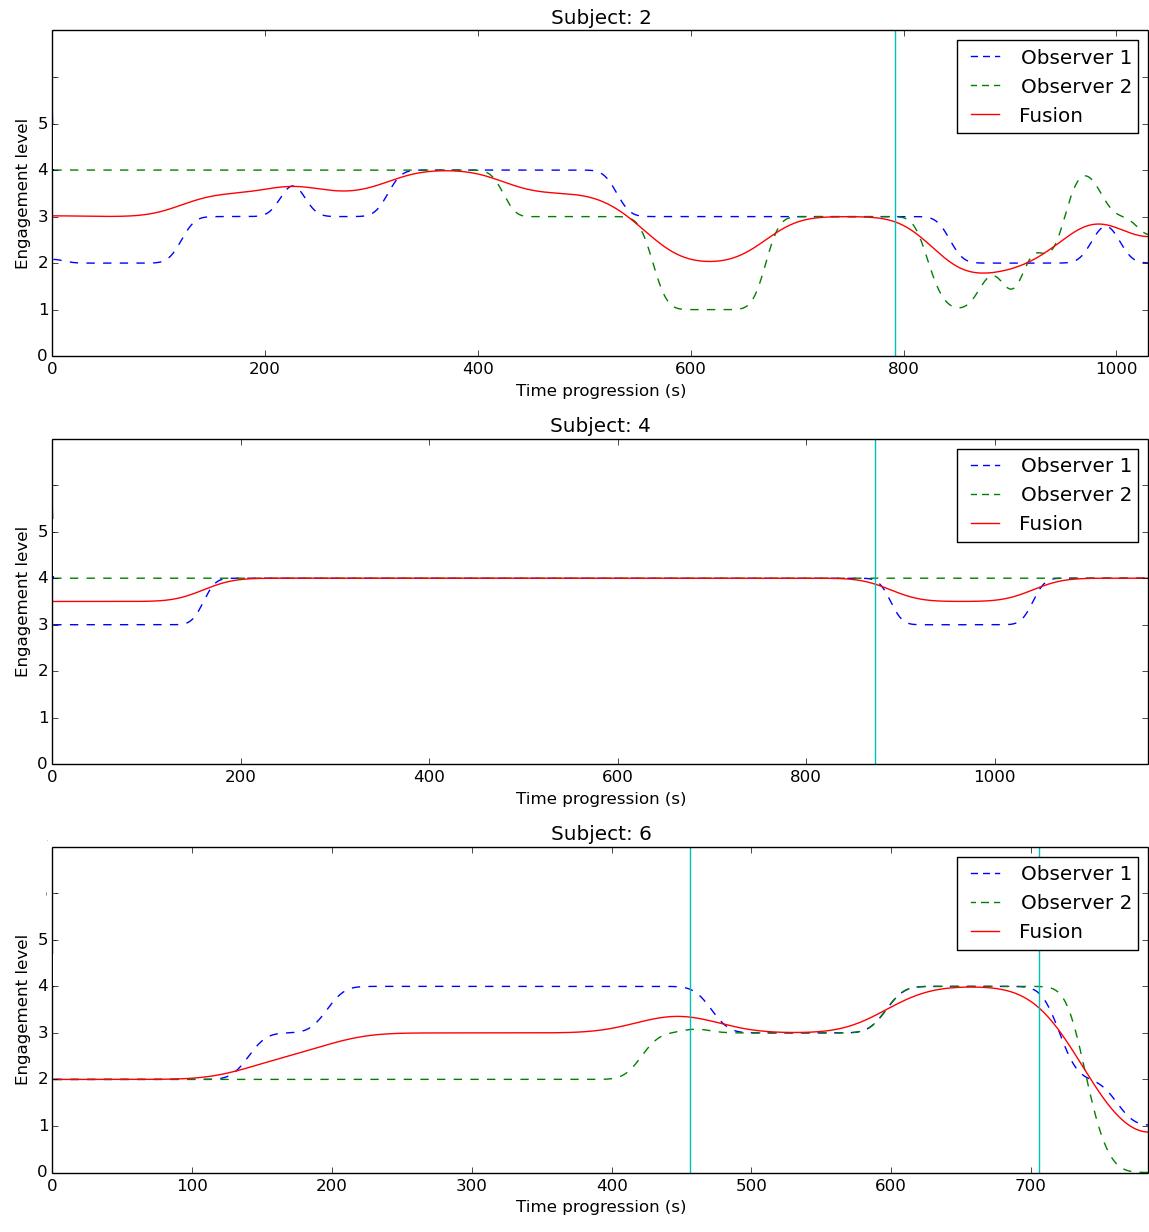
\includegraphics[width=0.6\textwidth]{figures/GT1.png}
    \label{fig:GT1}
\end{figure}
\newpage
\begin{figure}[h!]
    \centering
    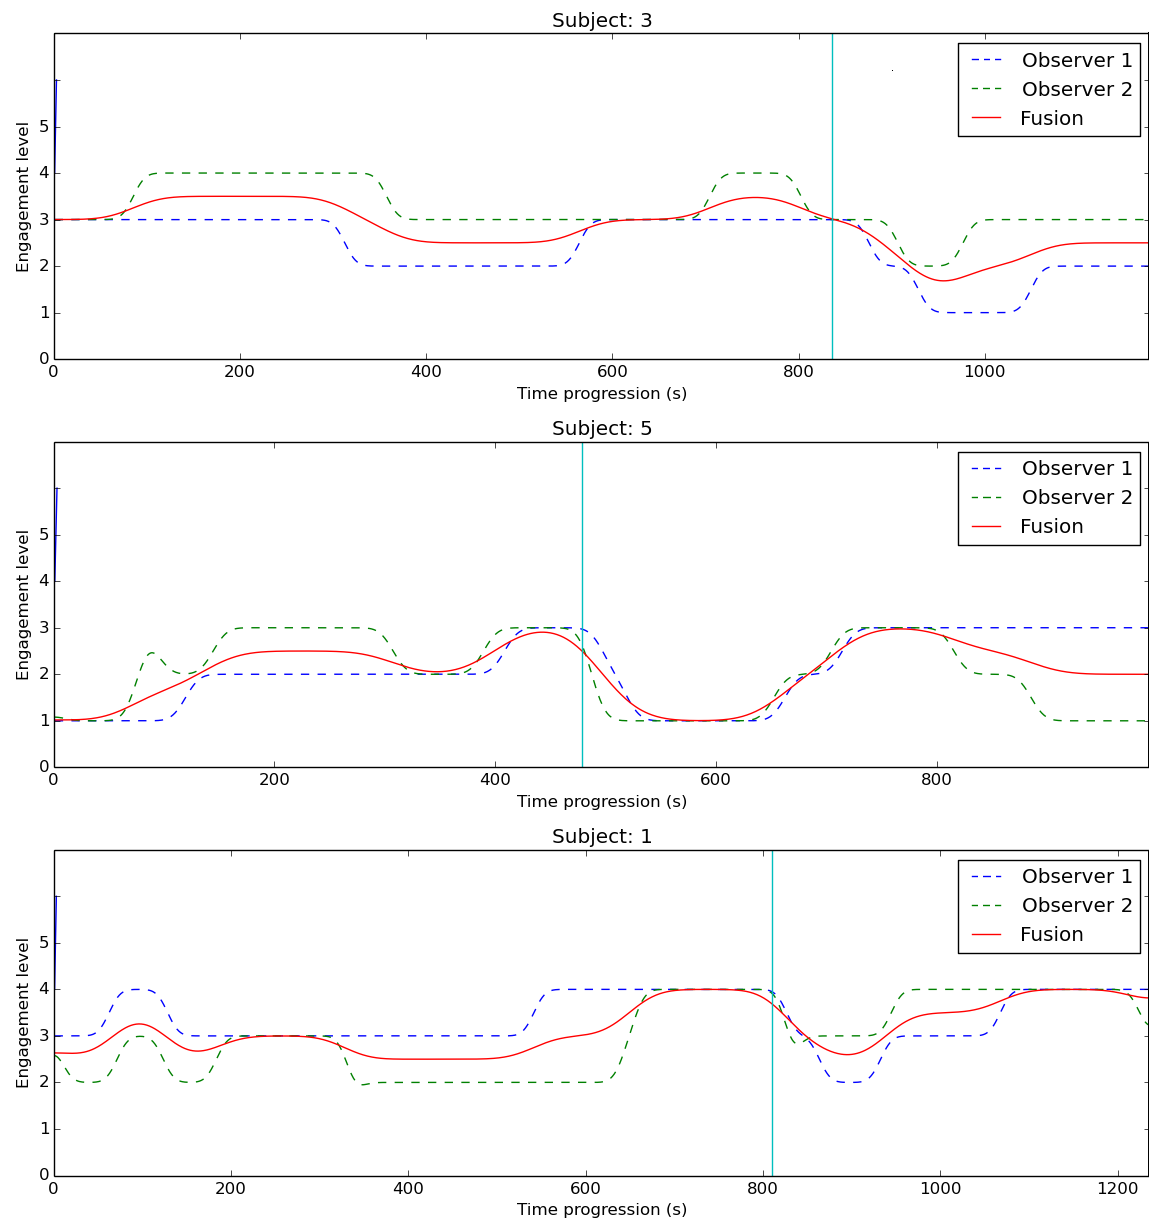
\includegraphics[width=0.6\textwidth]{figures/GT2.png}
    \label{fig:GT2}
    \caption{The 6 Ground Truth acquired during the experiments. The vertical lines indicate the switch to the story telling activity}\label{fig:GTTotal}
\end{figure}

	
\lstinputlisting[basicstyle=\ttfamily\scriptsize,frame=tb,caption=Ground Truth sanity and reliability test,label=zebra]{/home/ferran/Desktop/thesis/R_stuff/GToutput.txt}

\begin{equation} \label{eq:cronbach}
\alpha = {K \over K-1 } \left(1 - {\sum_{i=1}^K \sigma^2_{Y_i}\over \sigma^2_X}\right)
\end{equation}   
where $ \sigma^2_X $ is the variance of the observed total test scores, and $ \sigma^2_{Y_i} $ the variance of component i for the current sample of persons.

\begin{equation}\label{eq:chi}
 \chi^2 = \sum_{i=1}^{n} \frac{(O_i - E_i)^2}{E_i}  
\end{equation}

where $ O_i $ is the number of observations of type \textit{i}, \textit{N} the total number of observations and $ E_i $ the expected (theoretical) frequency of type \textit{i}.

\section{Movement and proximity across the two activities} \label{ap:across}
\lstinputlisting[basicstyle=\ttfamily\scriptsize, float=h,frame=tb,caption= Movement and proximity across activities using T-test,label=zebra]{/home/ferran/Desktop/thesis/R_stuff/acrossOut.txt}
\lstinputlisting[basicstyle=\ttfamily\scriptsize,float=h,frame=tb,caption= One-way repeated measures ANOVA test for proximity,label=zebra]{/home/ferran/Desktop/thesis/R_stuff/repeated1.txt}
\lstinputlisting[basicstyle=\ttfamily\scriptsize,float=h,frame=tb,caption= One-way repeated measures ANOVA test for movement,label=zebra]{/home/ferran/Desktop/thesis/R_stuff/repeated2.txt}


\lstinputlisting[basicstyle=\ttfamily\scriptsize,float=h,frame=tb,caption= Pearson's Chi-squared test result and residual measurements
,label=zebra]{/home/ferran/Desktop/thesis/R_stuff/chi.txt}

%\lstinputlisting[basicstyle=\ttfamily\scriptsize,float=h,frame=tb,caption=
%,label=zebra]{/home/ferran/Desktop/thesis/R_stuff/anovas.txt}




%   this is for BibTeX.  remove if you plan to write the references in the document
\bibliographystyle{plain}
\bibliography{refs}


%adds the bibliography to the table of contents
\addcontentsline{toc}{chapter}
         {\protect\numberline{Bibliography\hspace{-96pt}}}

\end{document}
